
\chapter{\textsf{``}Applied functional type theory\textsf{''}: A proposal\label{chap:Applied-functional-type}}

What exactly is the extent of \textsf{``}theory\textsf{''} that a software engineer
must know in order to be a proficient functional programmer? This
book proposes an answer to that question by presenting a coherent
body of theoretical knowledge that, in the author\textsf{'}s view, is the theory
that is practically useful for writing code. This body of knowledge
may be viewed as a new branch of computer science, called \textbf{\index{applied functional type theory}applied
functional type theory} (AFTT). This is the area of theoretical computer
science serving the practical needs of functional programmers working
as software engineers.

It is for those practitioners, rather than for academic researchers,
that this book sets out to examine the functional programming inventions
over the last 30 years, such as the \textquotedblleft functional pearls\textquotedblright{}
papers\footnote{\texttt{\href{https://wiki.haskell.org/Research_papers/Functional_pearls}{https://wiki.haskell.org/Research\_papers/Functional\_pearls}}}
and various online tutorials, in order to determine the scope of theoretical
material that has demonstrated its pragmatic usefulness and thus belongs
to AFTT. This book is a first step towards formulating AFTT from the
ground up, motivating and rigorously deriving all key results.

In this book, code examples are written in Scala because the author
is fluent in that language. However, most of the material will work
equally well in Haskell, OCaml, and other FP languages. This is because
the science of functional programming, called AFTT, is not a set of
tricks specific to Scala or Haskell. An advanced user of any functional
programming language will have to face the same questions and struggle
with the same practical issues.

\section{AFTT is not covered by courses in computer science}

Traditional courses of computer science (algorithms and data structures,
complexity theory, distributed systems, databases, network systems,
compilers, operating systems) are largely not relevant to AFTT. Courses
in programming language theory are more relevant but are not presented
at an appropriate level. To an academic computer scientist, the theory
behind Haskell is the version of $\lambda$-calculus known as\index{System F_{omega}@System $F_{\omega}$}
\textsf{``}System $F_{\omega}$\textsf{''}.\footnote{\texttt{\href{https://babel.ls.fi.upm.es/~pablo/Papers/Notes/f-fw.pdf}{https://babel.ls.fi.upm.es/$\sim$pablo/Papers/Notes/f-fw.pdf}}}
This theory guided the design of the Haskell language and defines
rigorously what a Haskell program means in a mathematical sense. The
theory behind Scala is the \textsf{``}dependent object type\textsf{''} (DOT) calculus.\footnote{\texttt{\href{https://www.scala-lang.org/blog/2016/02/03/essence-of-scala.html}{https://www.scala-lang.org/blog/2016/02/03/essence-of-scala.html}}}\index{dependent object type (DOT) calculus}
That theory guided the design of Scala version 3.

However, a practicing Haskell or Scala programmer is not concerned
with designing Haskell or Scala, or with proving theoretical properties
of those languages. Instead, the programmer is mainly concerned with
\emph{using} a chosen programming language to write code. 

Proving type-theoretical properties of System $F_{\omega}$ or DOT
will not actually help programmers to write code. So, these theories
are outside the scope of AFTT. Functional programming does not require
graduate-level theoretical studies.

As an example of theoretical material that \emph{is} within the scope
of AFTT, consider applicative functors (Chapter~\ref{chap:8-Applicative-functors,-contrafunc}).\index{applicative functors}
It is essential for a practicing functional programmer to be able
to recognize and use applicative functors. An applicative functor
is a data structure specifying declaratively a set of operations that
can run independently of each other. Programs may combine these operations,
for example, to execute them in parallel, or to refactor the program
for better maintainability.

To use this functionality, the programmer must begin by checking whether
a given data structure satisfies the laws of applicative functors.
In a given application, a data structure may be dictated in part by
the business logic rather than by a programmer\textsf{'}s choice. The programmer
first writes down the type of that data structure and the code implementing
the required methods; then checks that the laws hold. The data structure
may need to be adjusted in order to fit the definition of an applicative
functor or to make the laws hold.

So, before starting to write the actual code, the programmer needs
to perform a certain amount of symbolic derivations. That work can
be done using pen and paper, writing equations in a mathematical notation.
Once the applicative laws are verified, the programmer proceeds to
write code.

The mathematical proofs and derivations assure that the chosen data
structure will satisfy the laws of applicative functors, no matter
how the rest of the program is written. So, for example, it is assured
that the relevant effects can be automatically parallelized and will
still work correctly. In this way, AFTT directly guides the programmer
and helps write correct code.

Applicative functors were discovered by practitioners who were using
Haskell in programs such as parser combinators, compilers, and domain-specific
languages for parallel computations. However, applicative functors
are not a feature of Haskell: they can be used in Scala or any other
functional programming language. And yet, no standard computer science
textbook defines applicative functors, motivates their laws, explores
their structure on examples, or shows data structures that are \emph{not}
applicative functors and explains why. Books on category theory rarely
mention applicative functors (known in mathematics as \textsf{``}lax monoidal\textsf{''}
functors\footnote{\texttt{\href{https://en.wikipedia.org/wiki/Monoidal_functor}{https://en.wikipedia.org/wiki/Monoidal\_functor}}}).

\section{AFTT is not category theory, type theory, or formal logic}

It appears that AFTT includes a small selection of results from category
theory, formal logic, and type theory. However, software engineers
would not benefit from traditional academic courses in these subjects,
because their presentation is too abstract and at the same time lacks
specific results necessary for practical programming. Today\textsf{'}s academic
courses answer questions that academic computer scientists have, not
questions that practicing software engineers have.

There exist several books intended as presentations of category theory
\textsf{``}for computer scientists\textsf{''}\footnote{\texttt{\href{https://www.amazon.com/dp/0262660717}{https://www.amazon.com/dp/0262660717}}}
or \textsf{``}for programmers\textsf{''}.\footnote{\texttt{\href{https://github.com/hmemcpy/milewski-ctfp-pdf}{https://github.com/hmemcpy/milewski-ctfp-pdf}}}
However, those books do not explain many concepts relevant to programming,
such as applicative or traversable functors. Instead, those books
dwell on concepts (e.g., limits, enriched categories, topoi) that
have no applications in practical functional programming today.

Typical questions in academic books are \textsf{``}Is $X$ an introduction
rule or an elimination rule\textsf{''} and \textsf{``}Does property $Y$ hold in non-small
categories or only in the category of sets\textsf{''}. Questions a Scala programmer
might ask are \textsf{``}Can we compute a value of type \lstinline!Either[Z, R => A]!
from a value of type \lstinline!R => Either[Z, A]!\textsf{''} and \textsf{``}Is the
type constructor \lstinline!F[A] = Option[(A,A,A)]! a monad or only
an applicative functor\textsf{''}. The scope of AFTT includes answering the
last two questions but \emph{not} the first two.

A software engineer hoping to understand the science of functional
programming will not find the concepts of filterable, applicative,
or traversable functors in any books on category theory, including
books intended for programmers. And yet, these concepts are necessary
to obtain mathematically correct implementations of \lstinline!filter!,
\lstinline!zip!, and \lstinline!fold!, which are important and widely
used operations.

To compensate for the lack of AFTT textbooks, programmers have written
many online tutorials for each other, trying to explain the theoretical
concepts necessary for practical work. The term \textsf{``}monad tutorial\textsf{''}
became infamous because so many were  posted online.\footnote{\texttt{\href{https://www.johndcook.com/blog/2014/03/03/monads-are-hard-because/}{https://www.johndcook.com/blog/2014/03/03/monads-are-hard-because/}}}
Tutorials were also written about applicative functors, traversable
functors, free monads, etc., showing a real unfulfilled need for presenting
the limited, practice-relevant theory in an applied setting. 

For example, \textsf{``}free monads\textsf{''} became popular in the Scala community
around 2015. Many talks about free monads were presented at Scala
engineering conferences, giving different implementation but never
formulating rigorously the properties required for a piece of code
to be a valid implementation of the free monad. Without knowing the
required mathematical properties of free monads, a programmer cannot
make sure that a given implementation is correct. However, books on
category theory define free monads in a way that is unsuitable for
programming applications: a free monad is an adjoint functor to a
forgetful functor from a Kleisli category to the category of sets.\footnote{\textsf{``}\emph{A monad is just a monoid in the category of endofunctors.
What\textsf{'}s the problem?}\textsf{''} as the joke goes. For background information
about that joke, see \texttt{\href{https://stackoverflow.com/questions/3870088/}{https://stackoverflow.com/questions/3870088/}}} Such \textsf{``}academic\textsf{''} definitions can be used neither as guidance for
writing code or checking code correctness, nor as a conceptual explanation
that a learner would find helpful.

Perhaps the best selection of AFTT tutorial material today can be
found in the Haskell Wikibooks.\footnote{\texttt{\href{https://en.wikibooks.org/wiki/Haskell}{https://en.wikibooks.org/wiki/Haskell}}}
However, those tutorials are incomplete and limited to explaining
the use of Haskell. Many of them are suitable neither as a first introduction
nor as a reference on AFTT. Also, the Haskell Wikibooks tutorials
rarely show any derivations of laws or explain the required techniques.

Apart from referring to some notions from category theory, AFTT also
uses concepts from type theory and formal logic. However, existing
textbooks on type theory and formal logic focus on domain theory and
proof theory \textemdash{} which presents a lot of information that
will be difficult to learn for practicing programmers and yet will
never be applicable in their daily work. At the same time, those academic
books never mention practical techniques used in many functional programming
libraries today, such as reasoning about and implementing quantified
types, types parameterized by type constructors, or partial type-level
functions (known as \textsf{``}typeclasses\textsf{''}).

The proper scope of AFTT is to help the programmer with practical
tasks such as:
\begin{enumerate}
\item Deciding whether two data types are equivalent and implementing the
isomorphism transformations. For example, the Scala type \lstinline!(A, Either[B, C])!
is equivalent to \lstinline!Either[(A, B), (A, C)]!, but the type
\lstinline!A => Either[B, C]! is \emph{not} equivalent to \lstinline!Either[A => B, A => C]!.
\item Checking whether a definition of a recursive type is \textsf{``}valid\textsf{''},
i.e., does not lead to infinite loops. A simple example of an \textsf{``}invalid\textsf{''}
recursive type definition is \lstinline!case class Bad(x: Bad)!.
A simple example of a \textsf{``}valid\textsf{''} recursive type is \lstinline!case class Good(x: Option[Good])!.
\item Deciding whether a function with a given type signature can be implemented.
For example, 
\begin{lstlisting}
def f[Z,A,R]: (R => Either[Z, A]) => Either[Z, R => A] = ???   // Cannot be implemented.
def g[Z,A,R]: Either[Z, R => A] => (R => Either[Z, A]) = ???   // Can be implemented.
\end{lstlisting}
\item Deriving an implementation of a function from its type signature and
checking required laws. For example, deriving the \lstinline!flatMap!
method and checking the laws for the \lstinline!Reader! monad,
\begin{lstlisting}
def flatMap[Z, A, B](r: Z => A)(f: A => Z => B): Z => B = ???
\end{lstlisting}
\item Deriving a simpler but equivalent code by calculating with functions,
equations, and laws.
\end{enumerate}
These are real-world applications of type theory and the Curry-Howard
correspondence, but existing books on type theory and logic do not
give practical recipes for performing these tasks.\footnote{Task 5 is addressed in several programming-oriented books such as
\emph{Pearls of functional algorithm design} by \index{Richard Bird}Richard
Bird (\texttt{\href{https://www.cambridge.org/9780521513388}{https://www.cambridge.org/9780521513388}}).}

Books such as \emph{Scala with Cats},\footnote{\texttt{\href{https://underscore.io/books/scala-with-cats/}{https://underscore.io/books/scala-with-cats/}}}
\emph{Functional programming simplified},\footnote{\texttt{\href{https://alvinalexander.com/scala/functional-programming-simplified-book}{https://alvinalexander.com/scala/functional-programming-simplified-book}}}
and \emph{Functional programming for mortals}\footnote{\texttt{\href{http://www.lulu.com/shop/search.ep?contributorId=1600066}{http://www.lulu.com/shop/search.ep?contributorId=1600066}}}
are primarily focused on explaining practical aspects of functional
programming and do not derive the mathematical laws for, e.g., applicative,
monadic, or traversable functors.

The only Scala-based AFTT textbook is \emph{Functional Programming
in Scala}.\footnote{\texttt{\href{https://www.manning.com/books/functional-programming-in-scala}{https://www.manning.com/books/functional-programming-in-scala}}}
It balances practical coding with theoretical developments and laws.
\emph{Program design by calculation}\footnote{\texttt{\href{http://www4.di.uminho.pt/~jno/ps/pdbc.pdf}{http://www4.di.uminho.pt/$\sim$jno/ps/pdbc.pdf}}}
is another (Haskell-oriented) AFTT book in progress. The present book
is written at about the same level but aims at better motivation for
mathematical concepts and a wider range of pedagogical examples that
help build the necessary intuition and facility with the techniques
of formal derivation. 

Figures~\ref{fig:Randomly-chosen-pages}\textendash \ref{fig:Randomly-chosen-pages-1}
illustrate the difference between AFTT books, programming books, and
academic science books, by showing randomly chosen pages from such
books. Programming-oriented books contain code examples and explanations
in words, but no formal derivations. Books on AFTT, as well as books
on mathematics and science, will typically show equations, diagrams,
and derivations in addition to example code. This book contains both
code examples and mathematical manipulations.

\begin{figure}
\begin{centering}
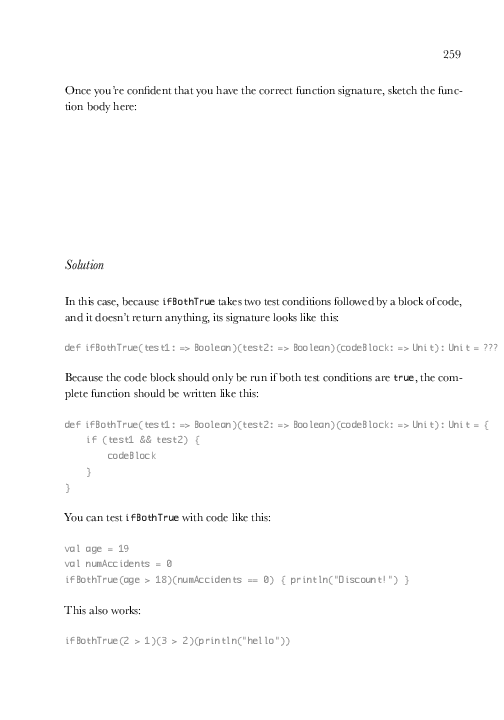
\includegraphics[height=2.51cm]{random-pages/random-pages-from-fpsimplified-pdf-00}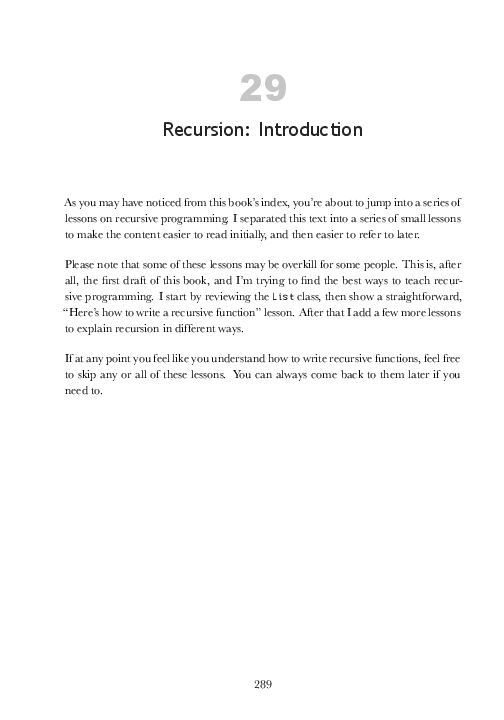
\includegraphics[height=2.51cm]{random-pages/random-pages-from-fpsimplified-pdf-01}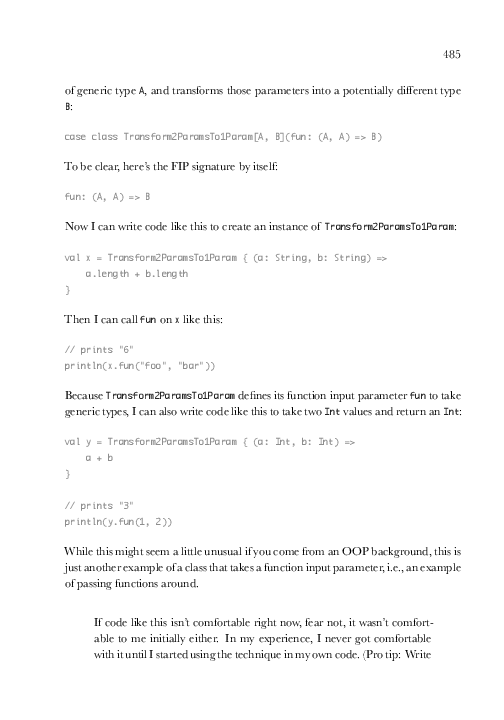
\includegraphics[height=2.51cm]{random-pages/random-pages-from-fpsimplified-pdf-02}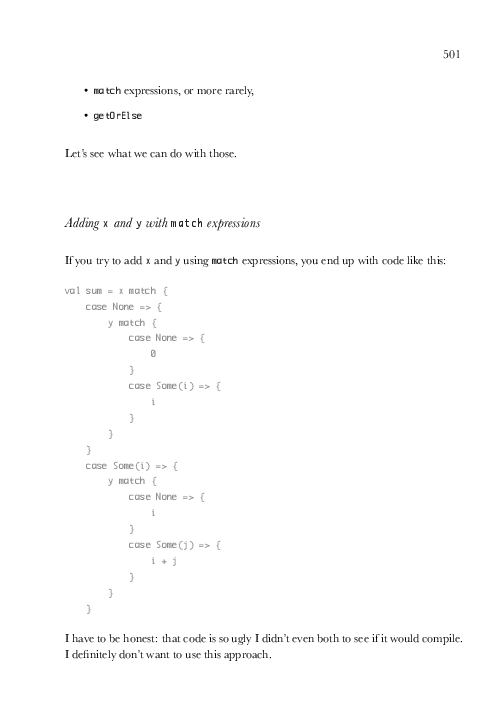
\includegraphics[height=2.51cm]{random-pages/random-pages-from-fpsimplified-pdf-03}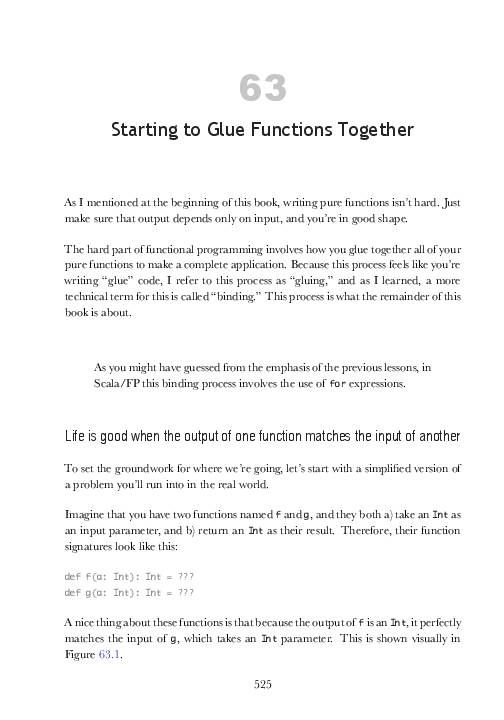
\includegraphics[height=2.51cm]{random-pages/random-pages-from-fpsimplified-pdf-04}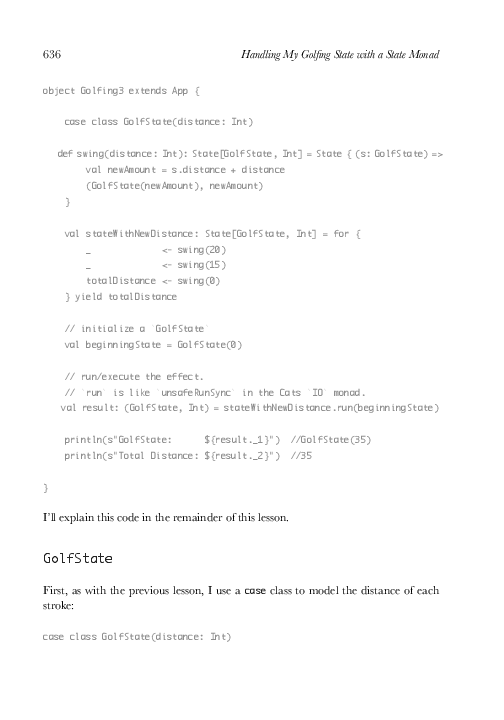
\includegraphics[height=2.51cm]{random-pages/random-pages-from-fpsimplified-pdf-05}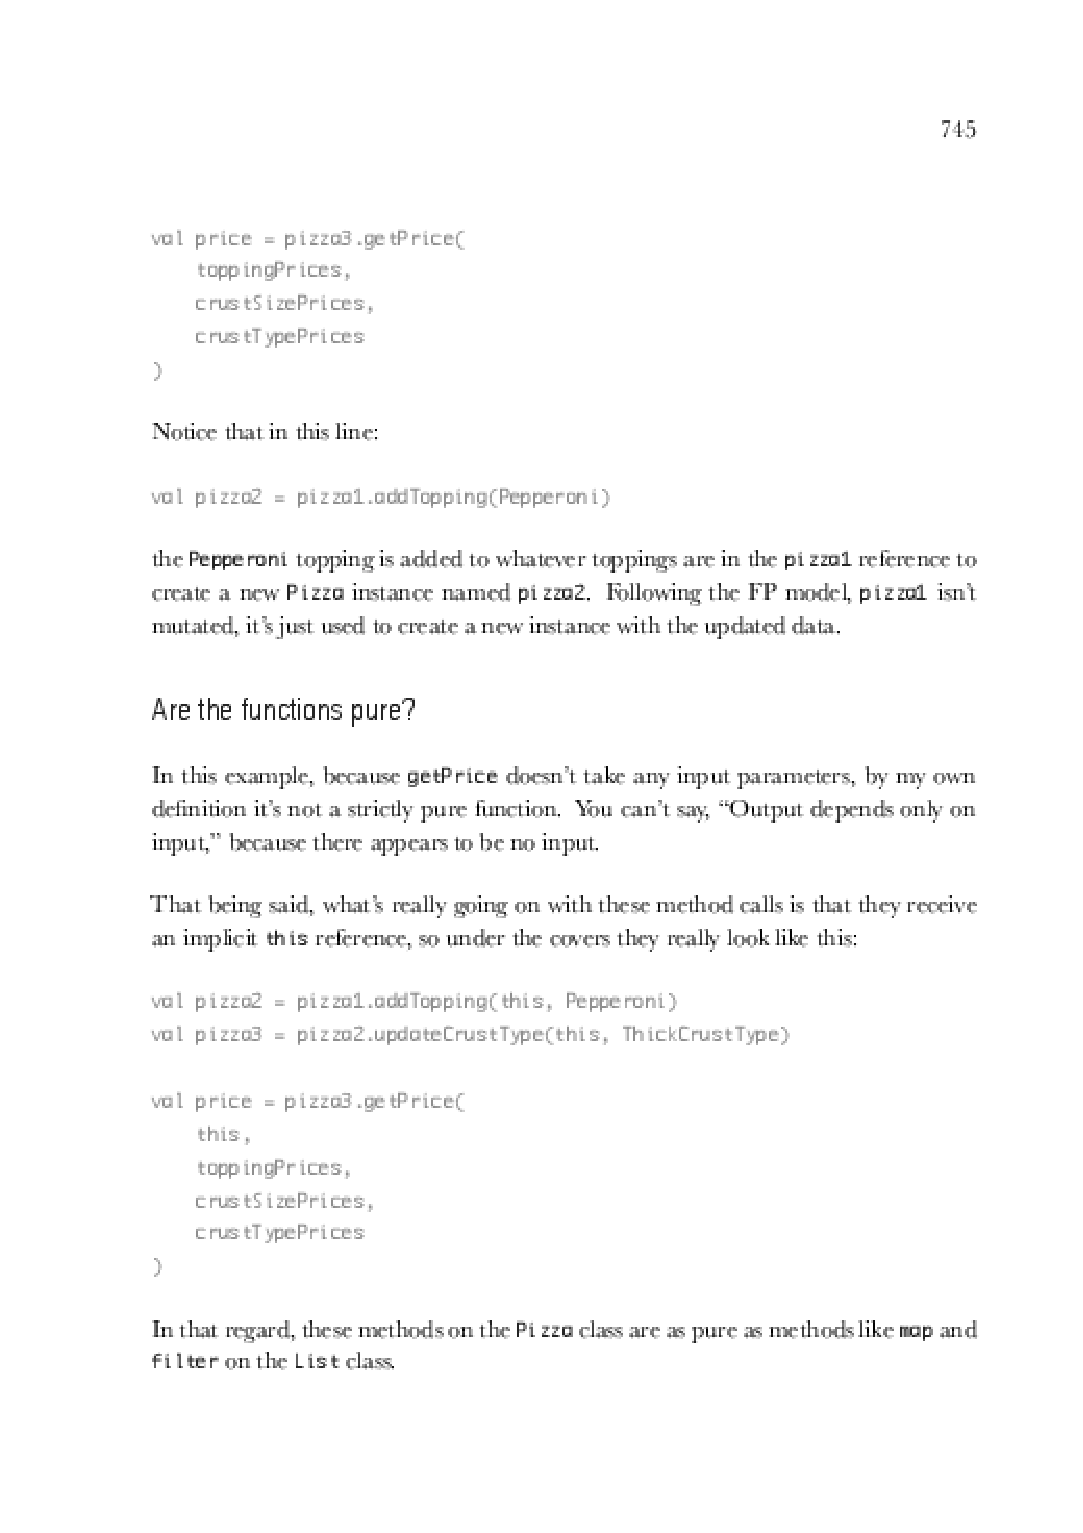
\includegraphics[height=2.51cm]{random-pages/random-pages-from-fpsimplified-pdf-06}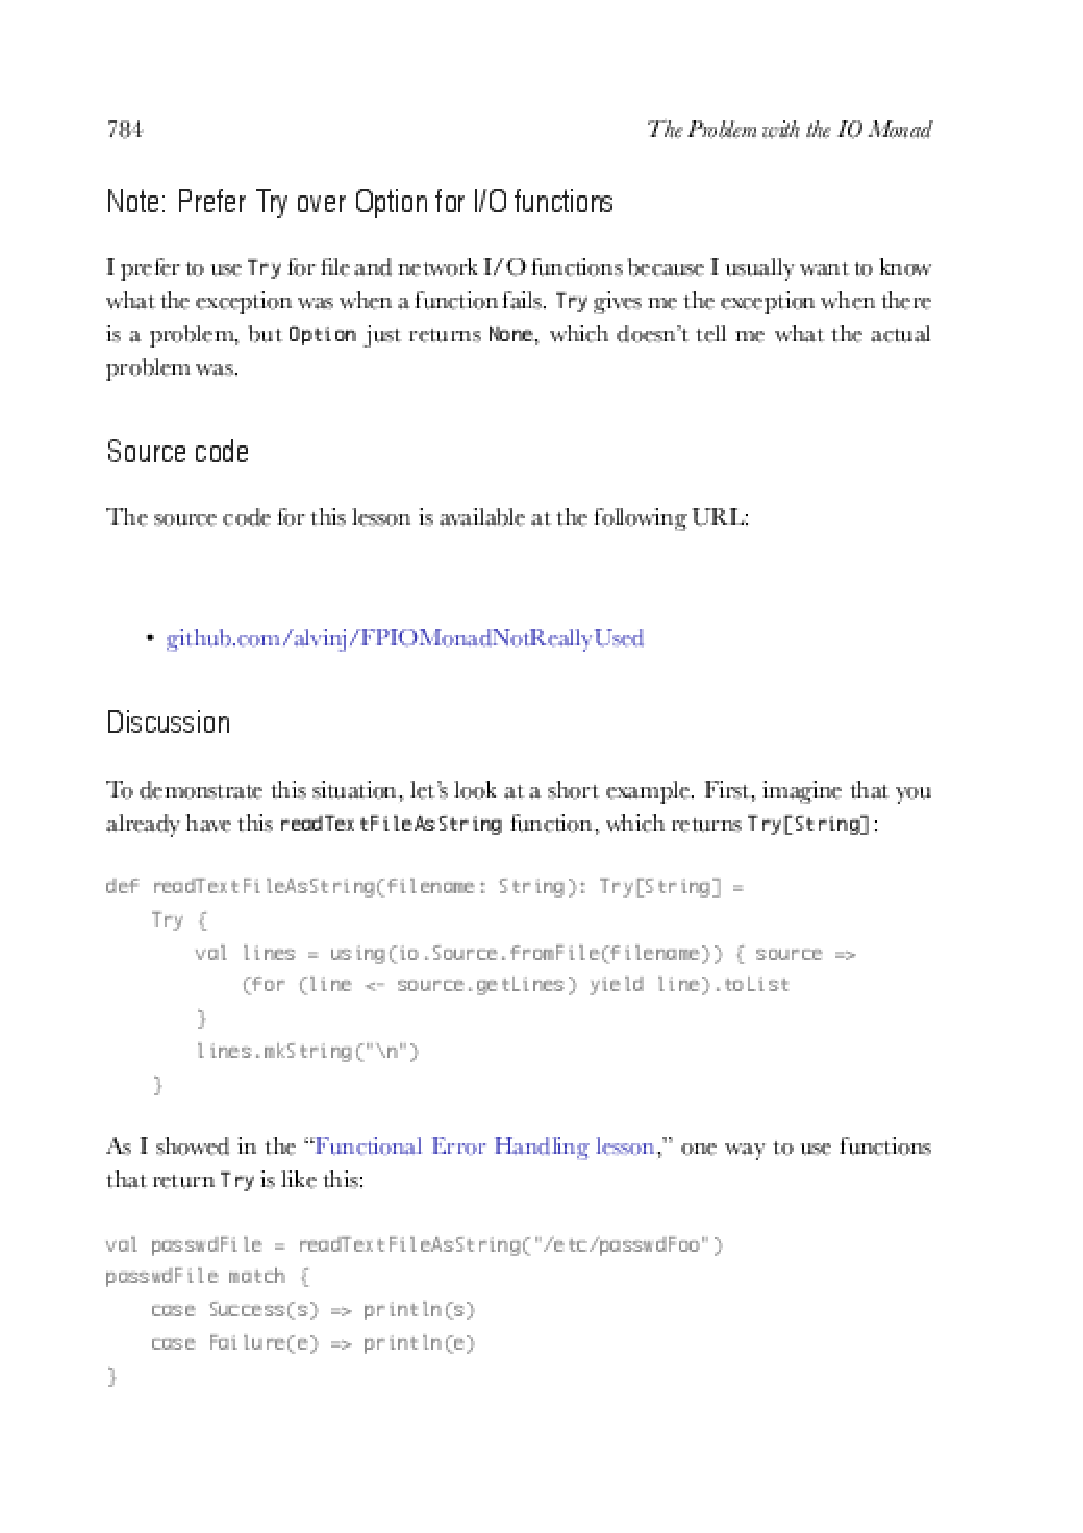
\includegraphics[height=2.51cm]{random-pages/random-pages-from-fpsimplified-pdf-07}
\par\end{centering}
\begin{centering}
\textsf{``}Functional programming simplified\textsf{''} by A.~Alexander
\par\end{centering}
\begin{centering}
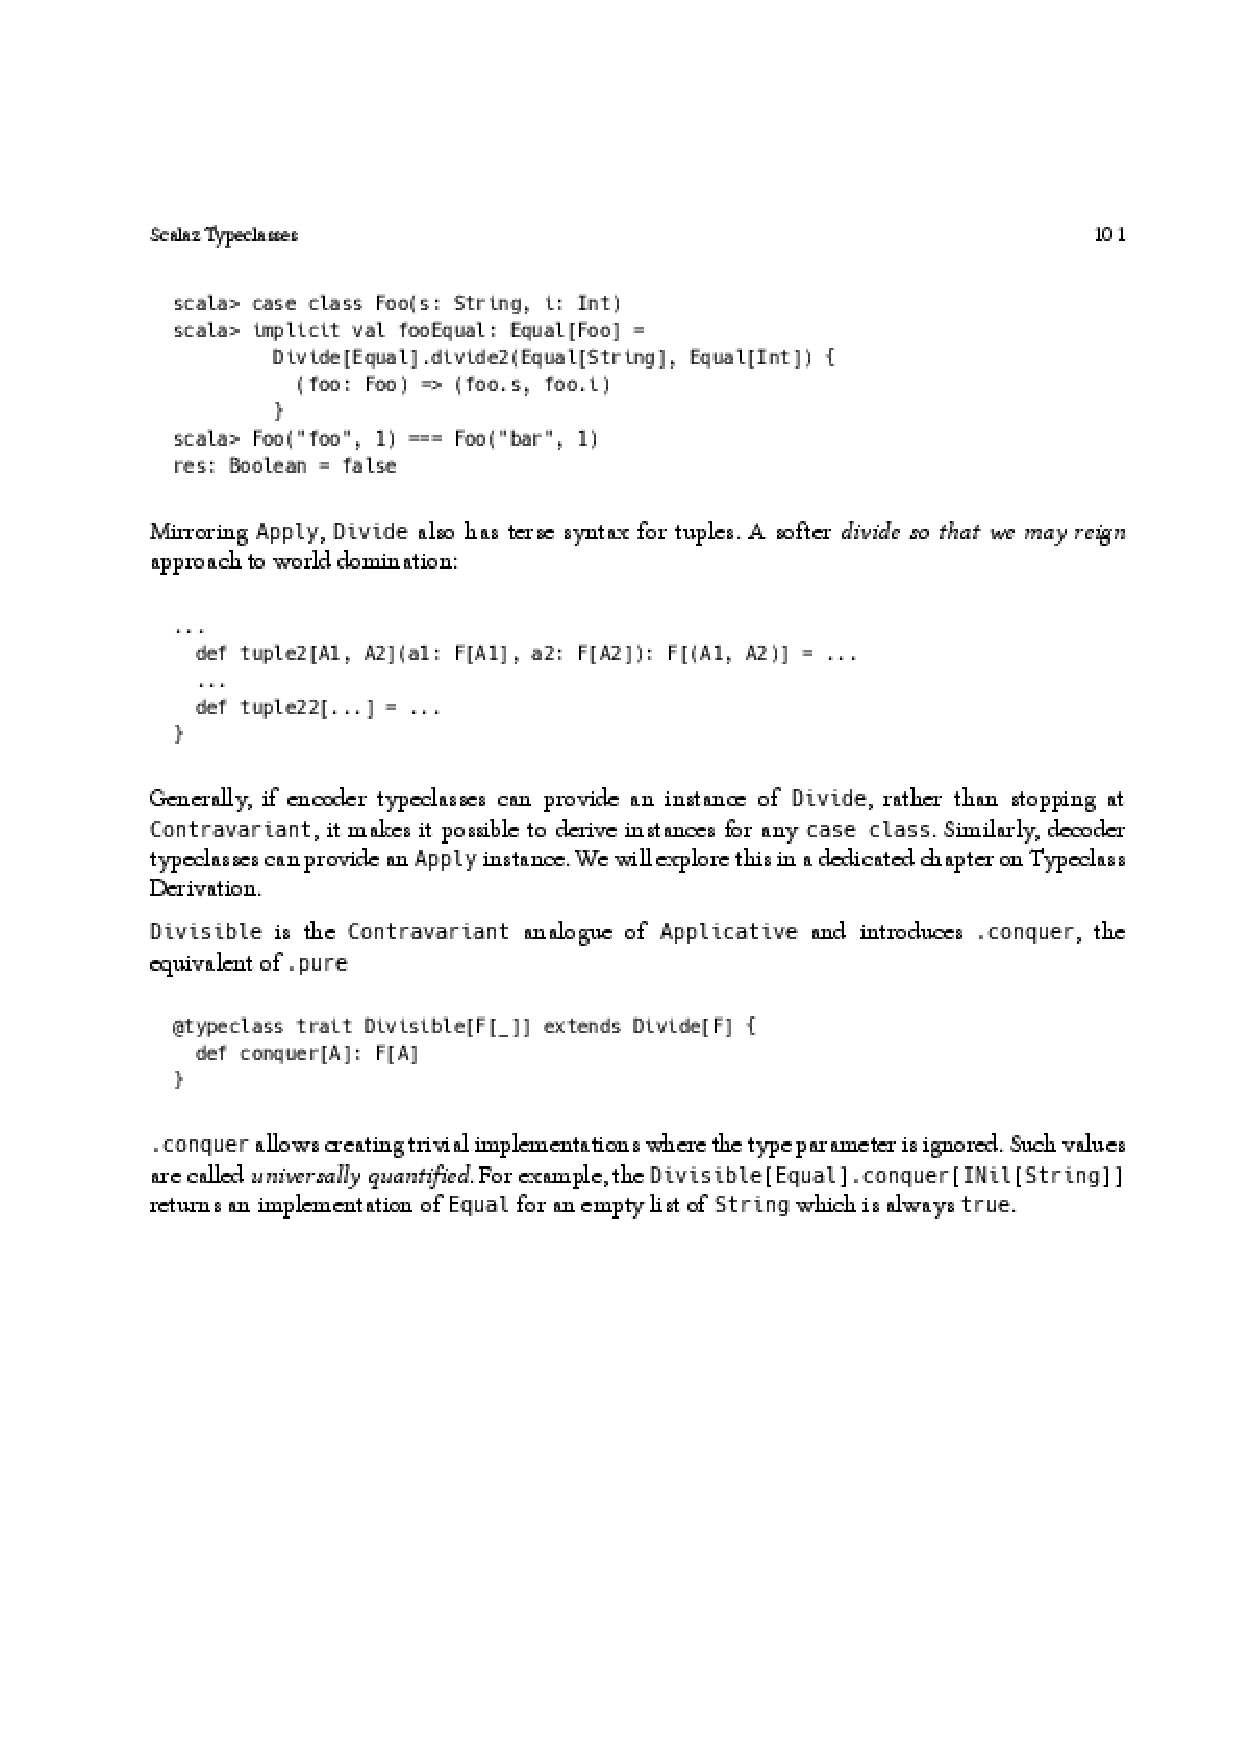
\includegraphics[height=2.51cm]{random-pages/random-pages-from-fpmortals-pdf-00}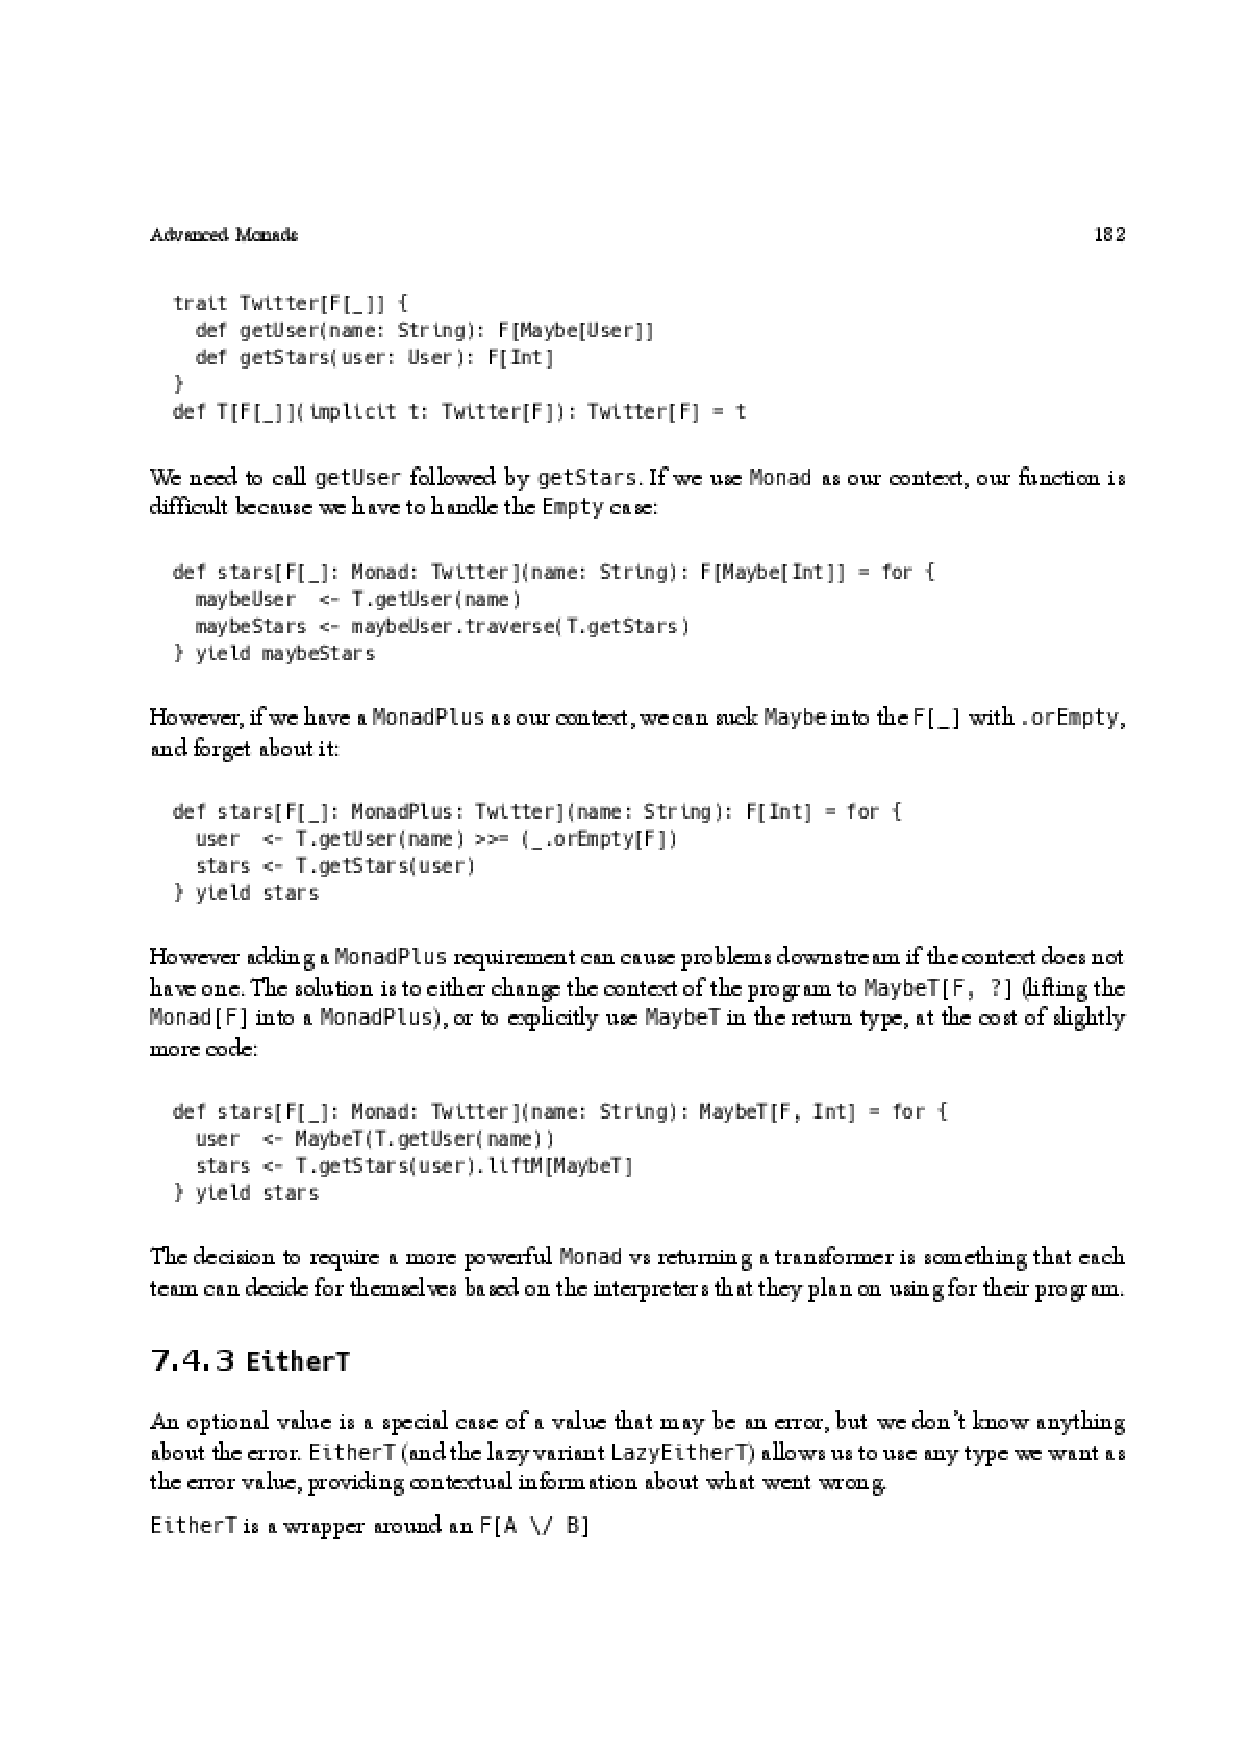
\includegraphics[height=2.51cm]{random-pages/random-pages-from-fpmortals-pdf-01}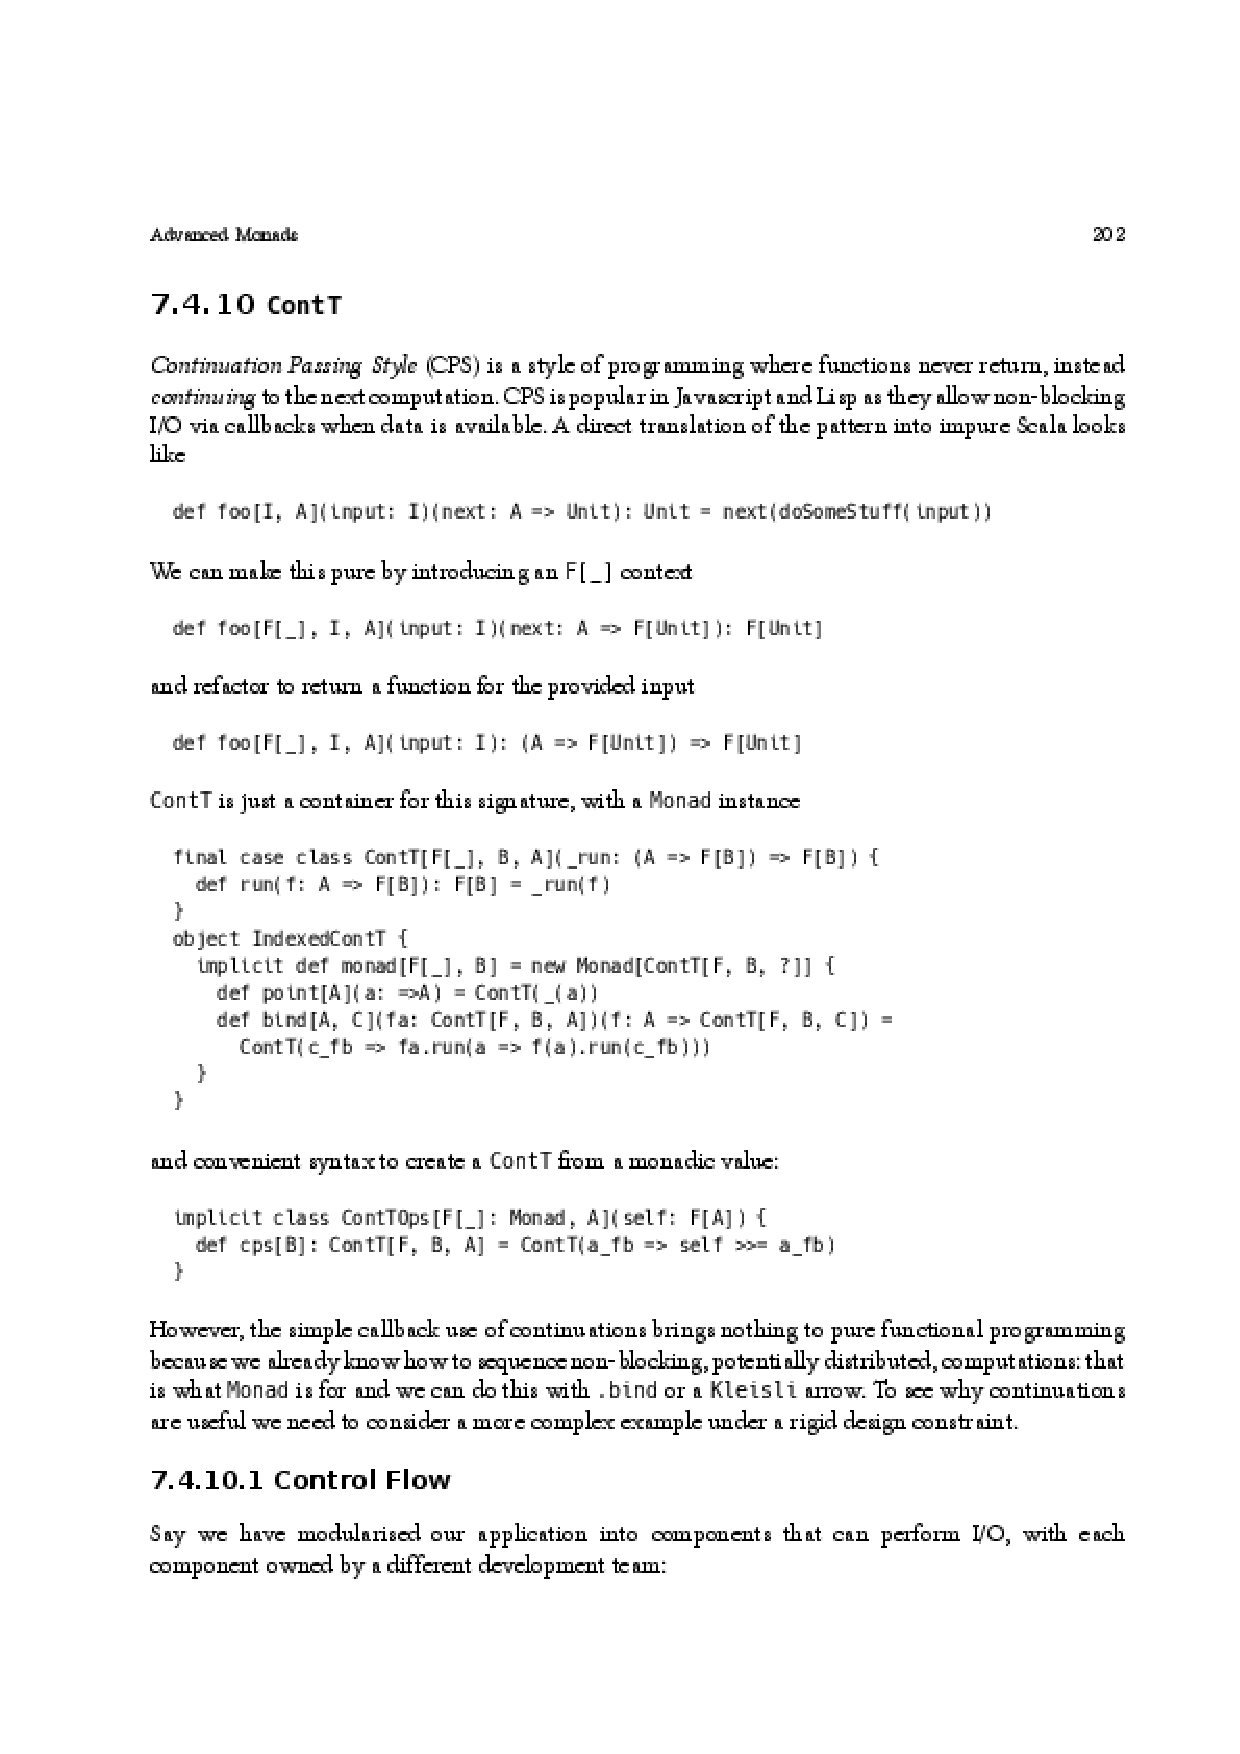
\includegraphics[height=2.51cm]{random-pages/random-pages-from-fpmortals-pdf-02}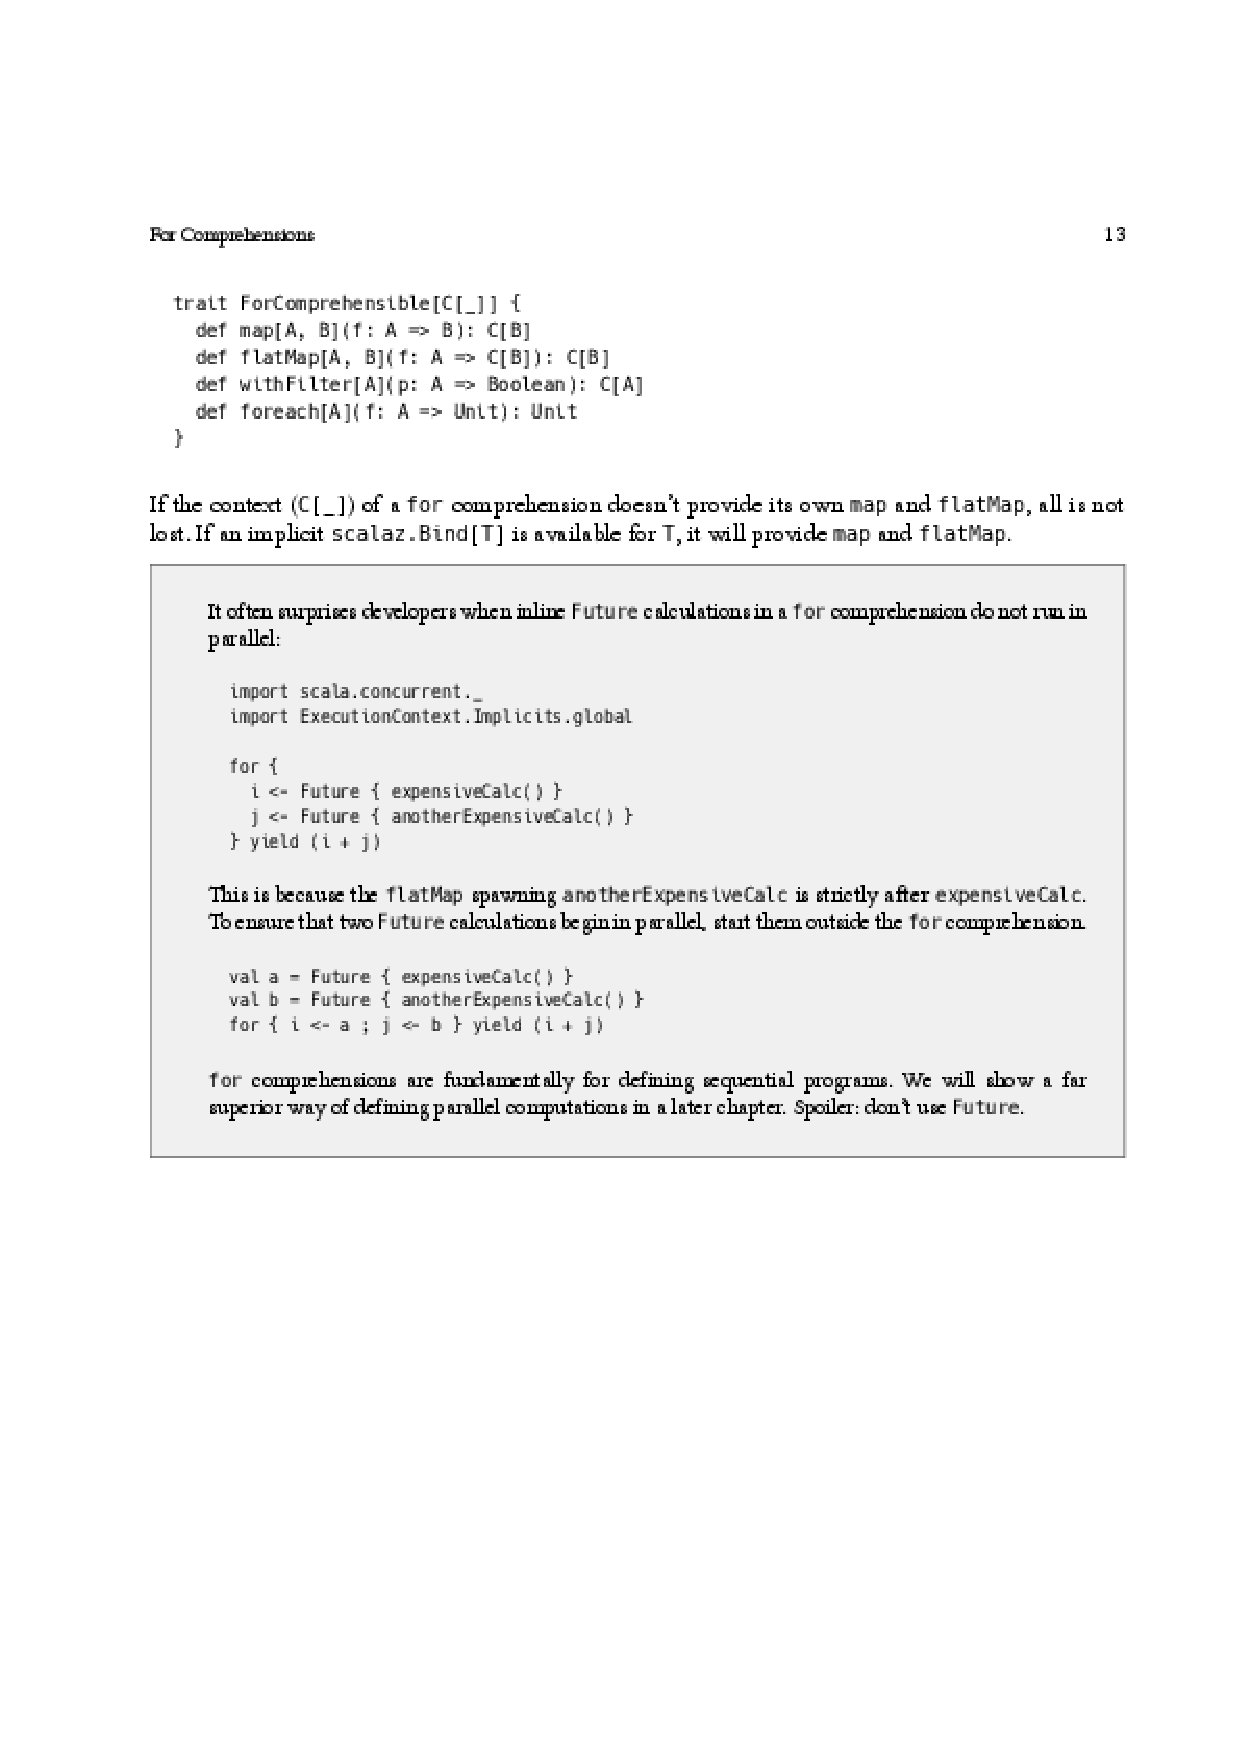
\includegraphics[height=2.51cm]{random-pages/random-pages-from-fpmortals-pdf-03}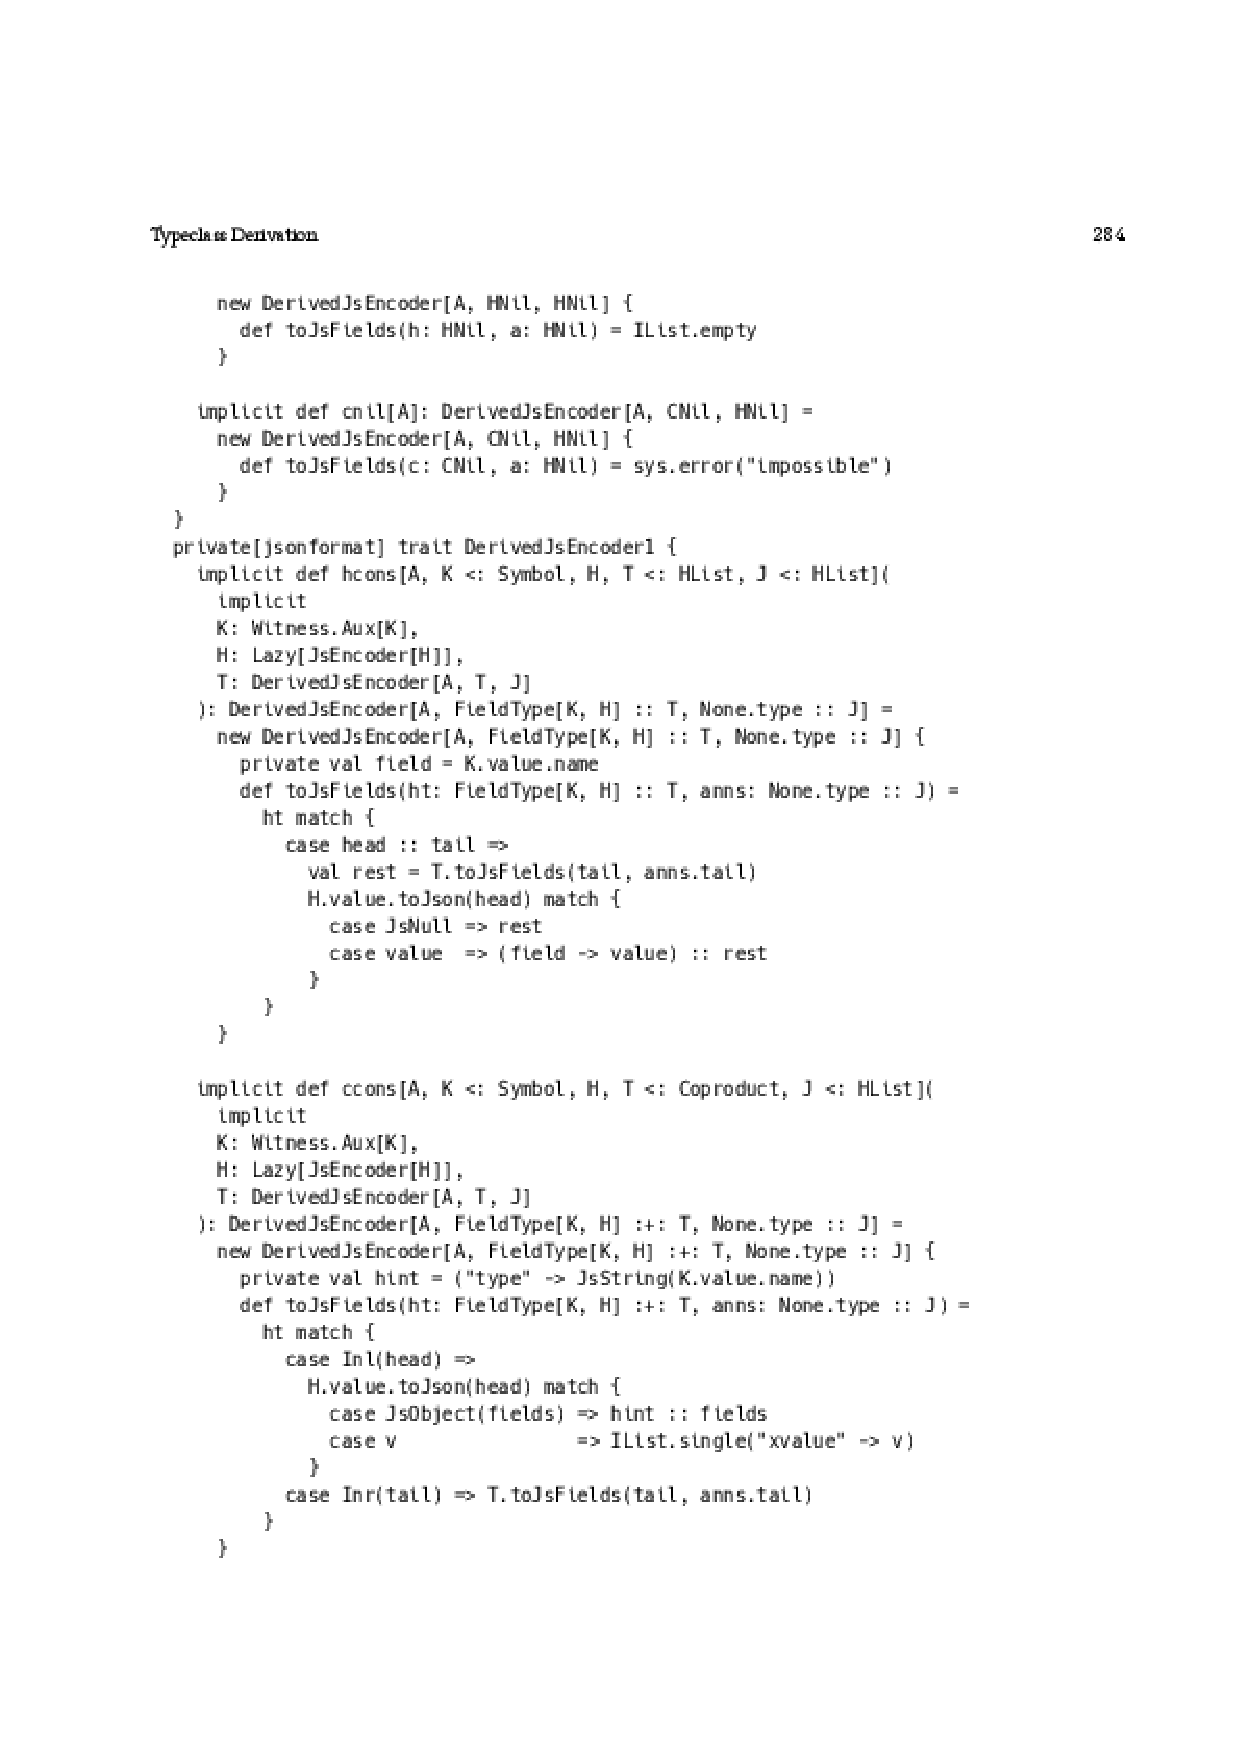
\includegraphics[height=2.51cm]{random-pages/random-pages-from-fpmortals-pdf-04}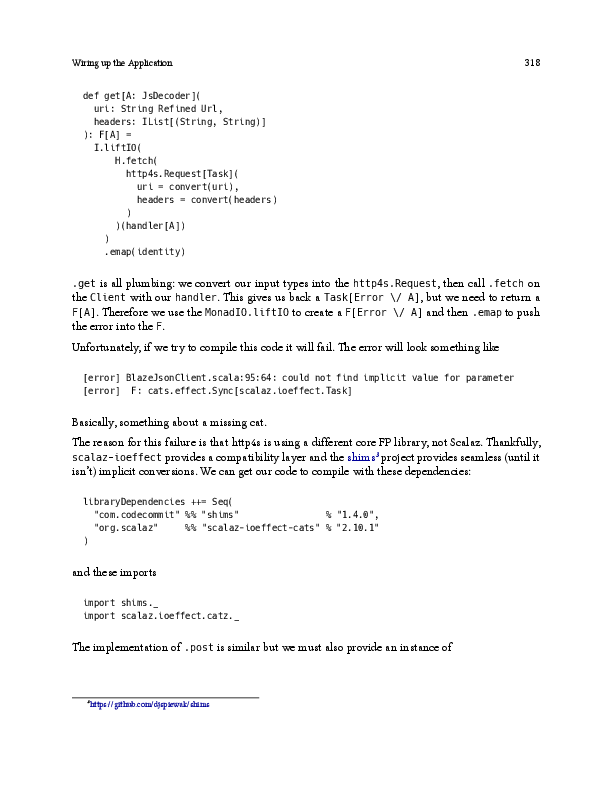
\includegraphics[height=2.51cm]{random-pages/random-pages-from-fpmortals-pdf-06}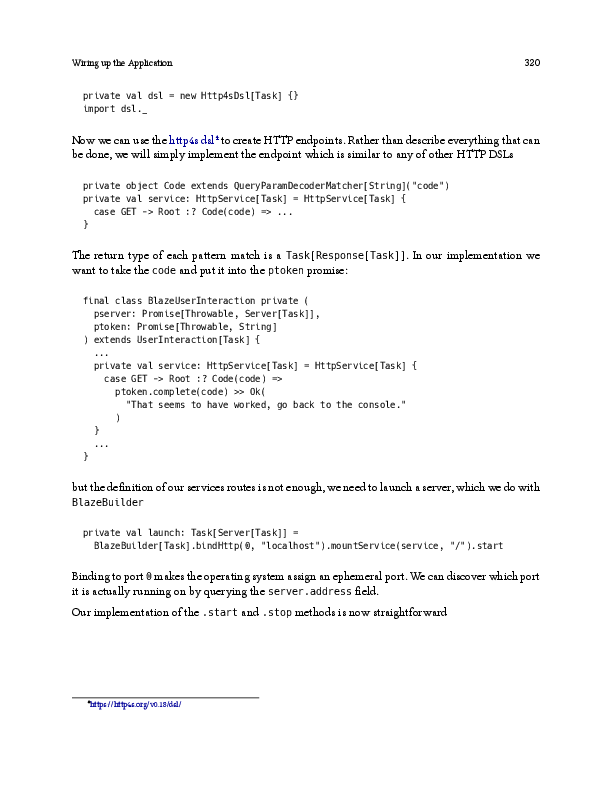
\includegraphics[height=2.51cm]{random-pages/random-pages-from-fpmortals-pdf-07}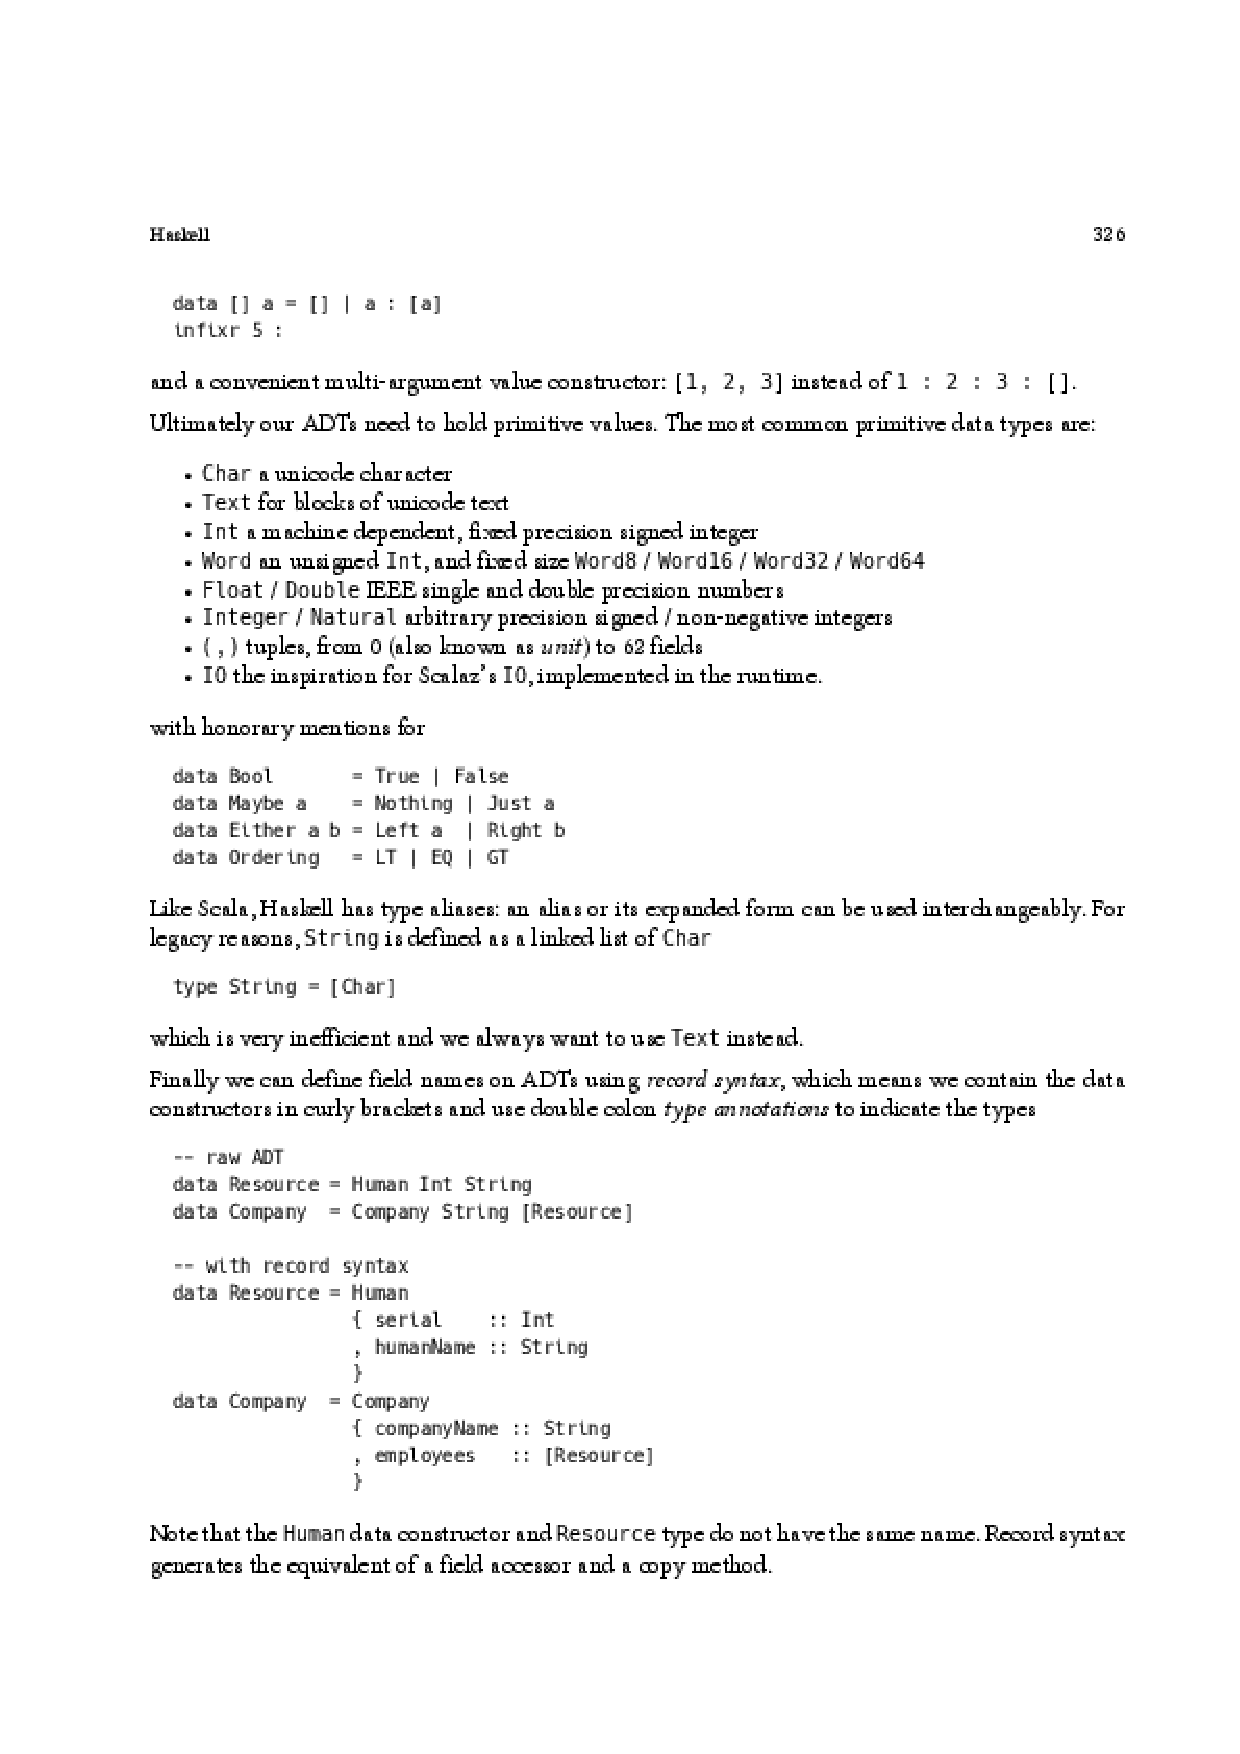
\includegraphics[height=2.51cm]{random-pages/random-pages-from-fpmortals-pdf-08}
\par\end{centering}
\begin{centering}
\textsf{``}Functional programming for mortals\textsf{''} by S.~Halliday
\par\end{centering}
\begin{centering}
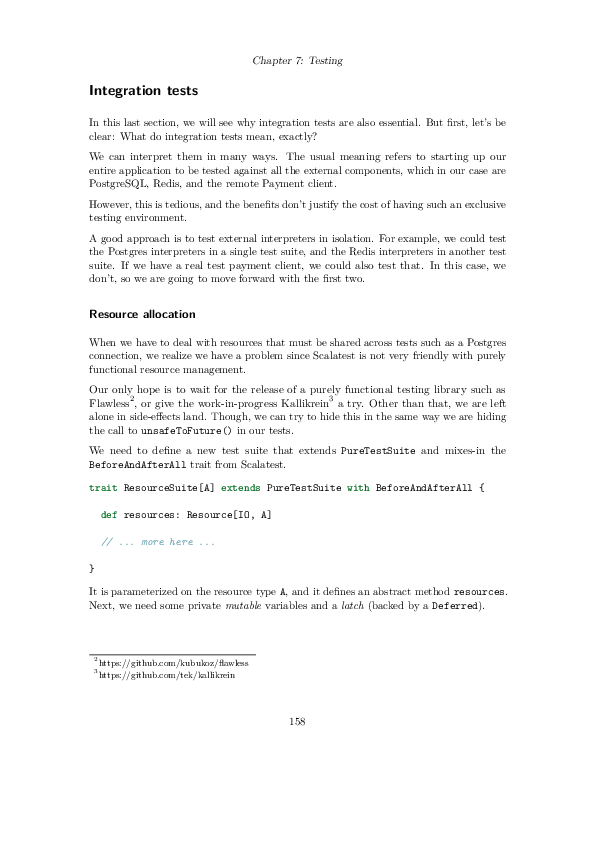
\includegraphics[height=2.51cm]{random-pages/random-pages-from-volpe-pdf-01}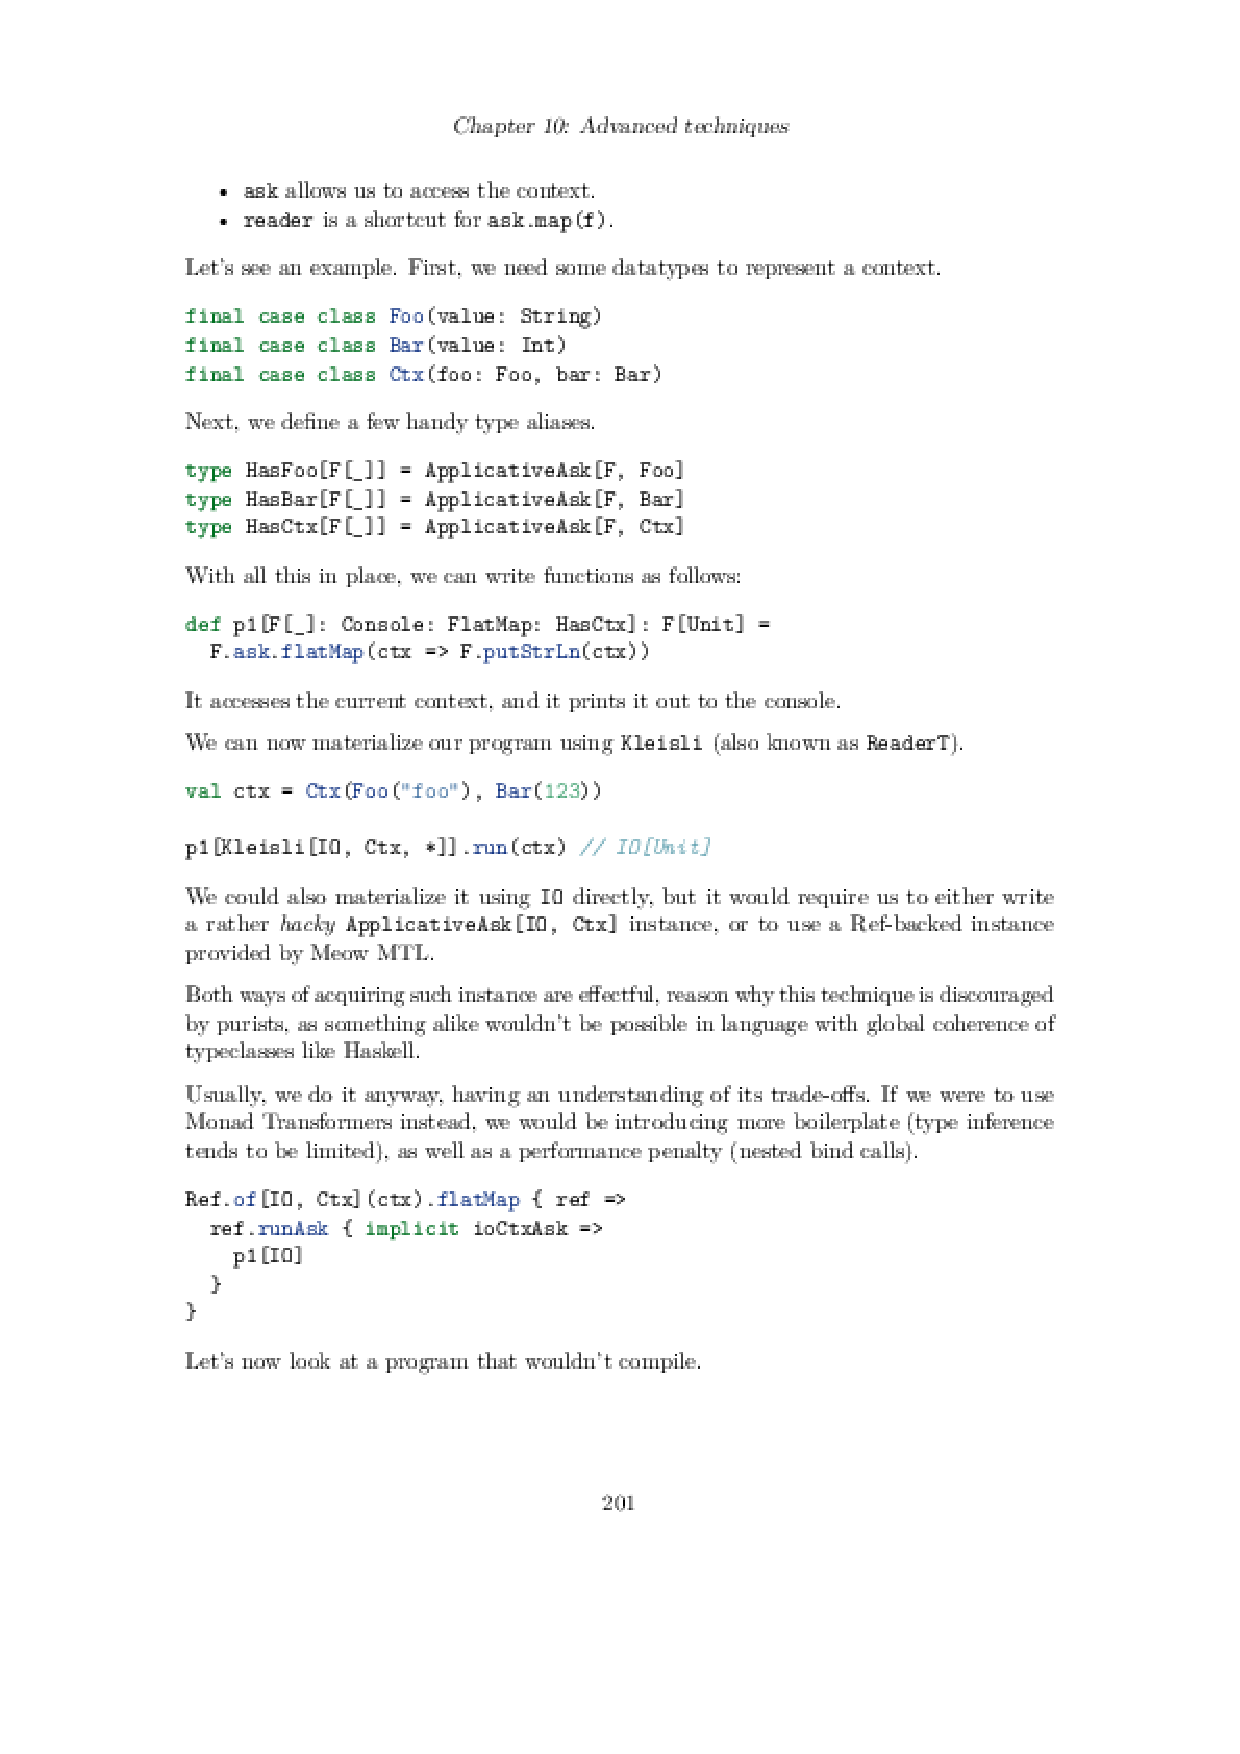
\includegraphics[height=2.51cm]{random-pages/random-pages-from-volpe-pdf-03}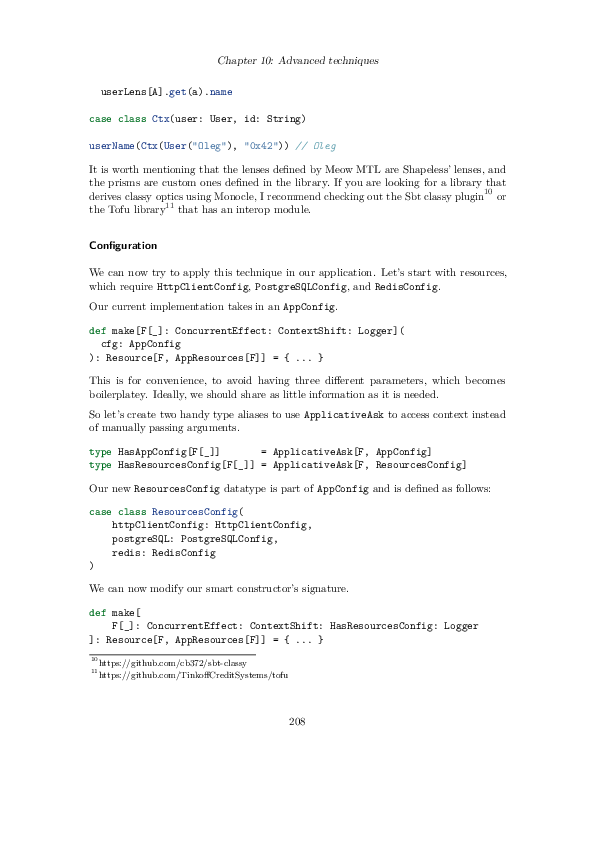
\includegraphics[height=2.51cm]{random-pages/random-pages-from-volpe-pdf-04}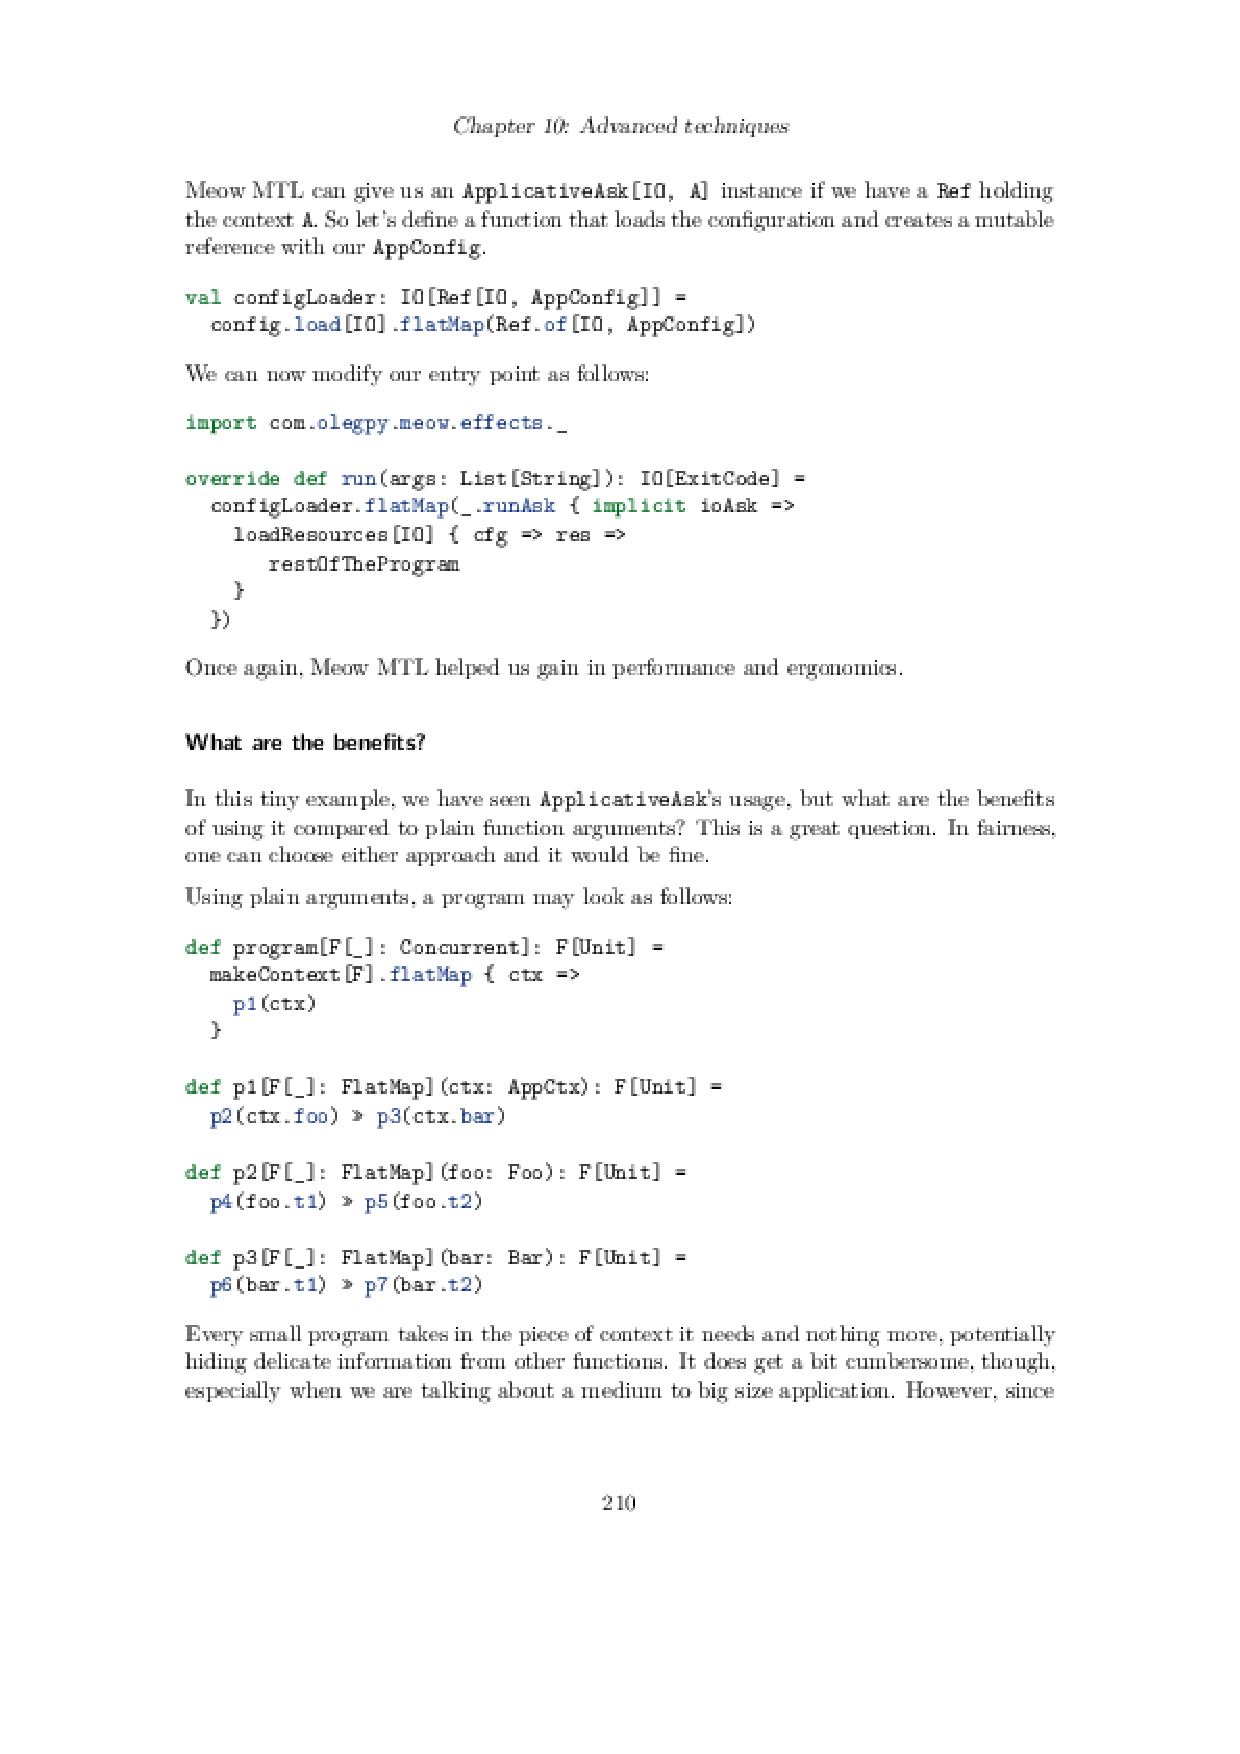
\includegraphics[height=2.51cm]{random-pages/random-pages-from-volpe-pdf-05}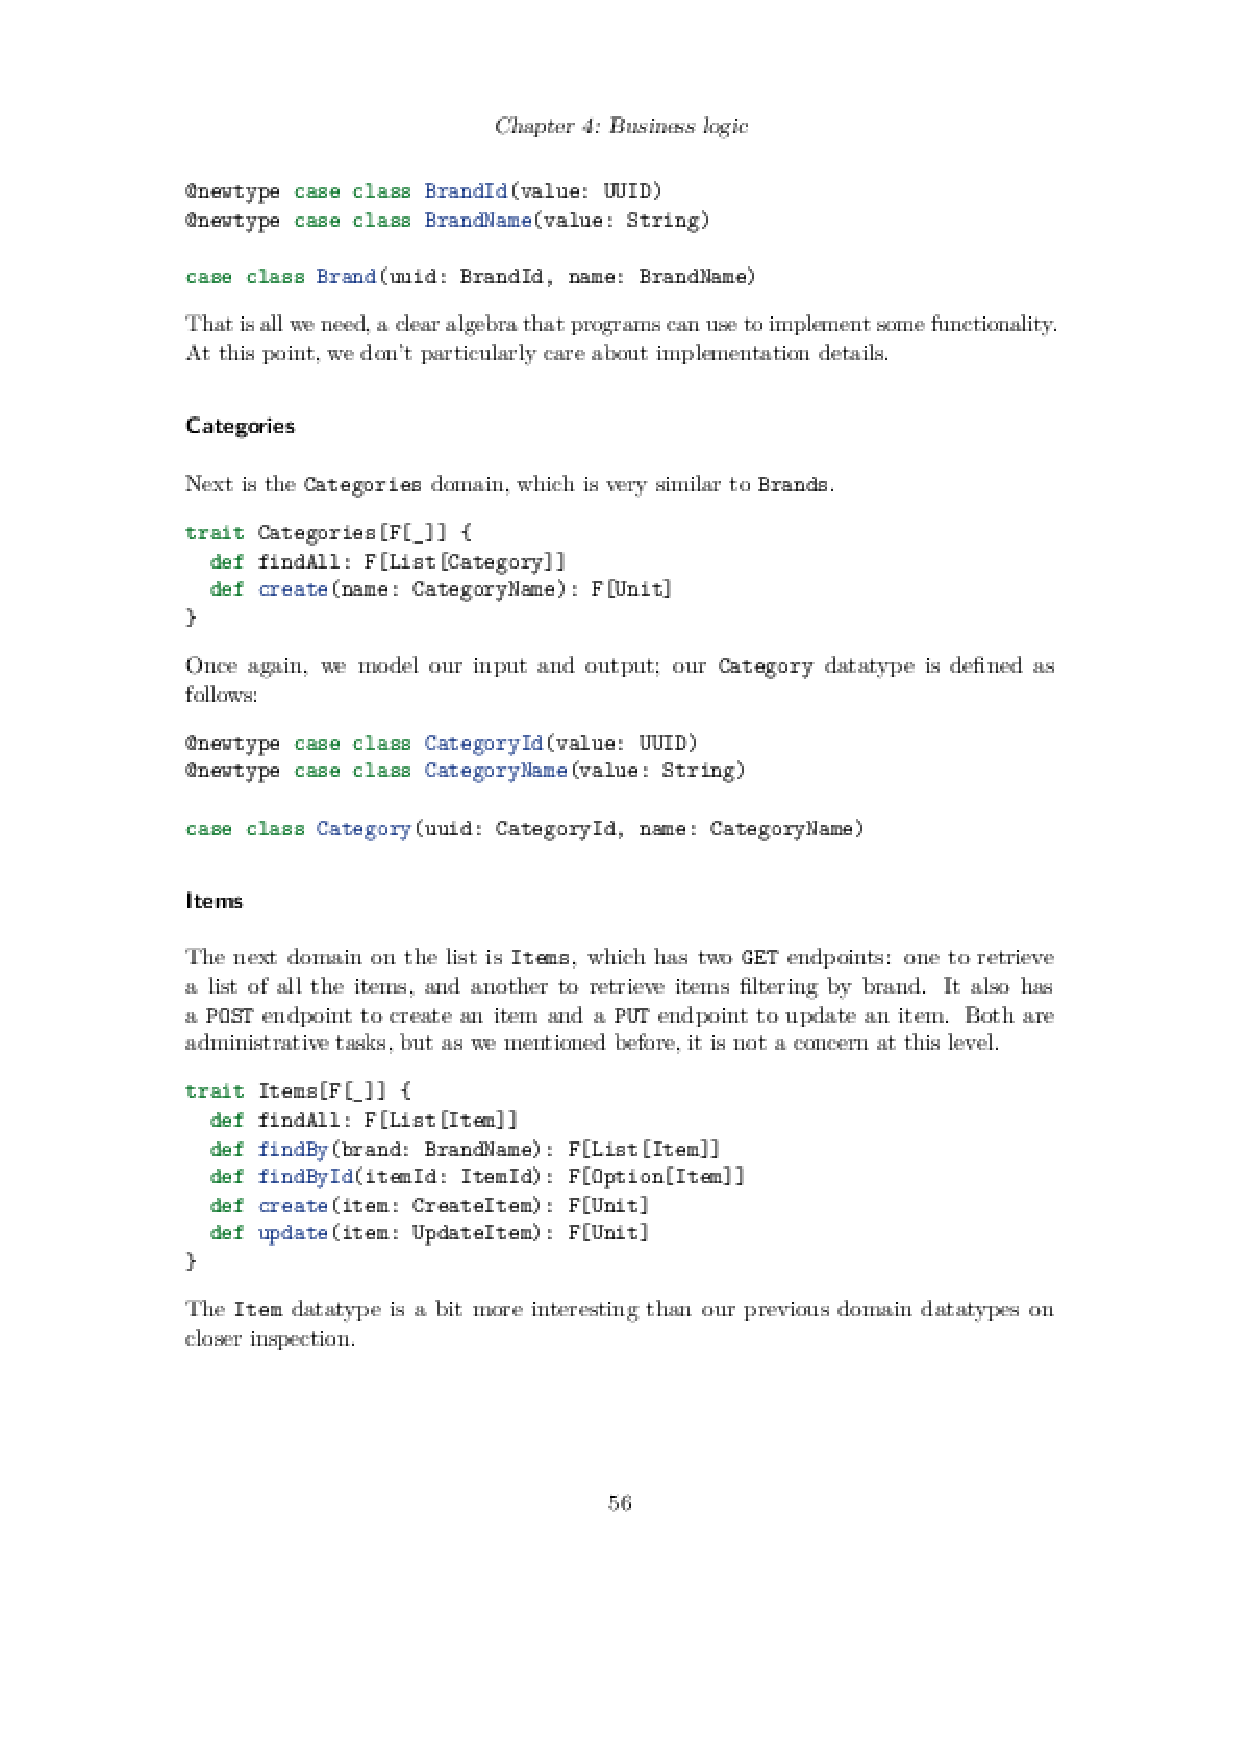
\includegraphics[height=2.51cm]{random-pages/random-pages-from-volpe-pdf-06}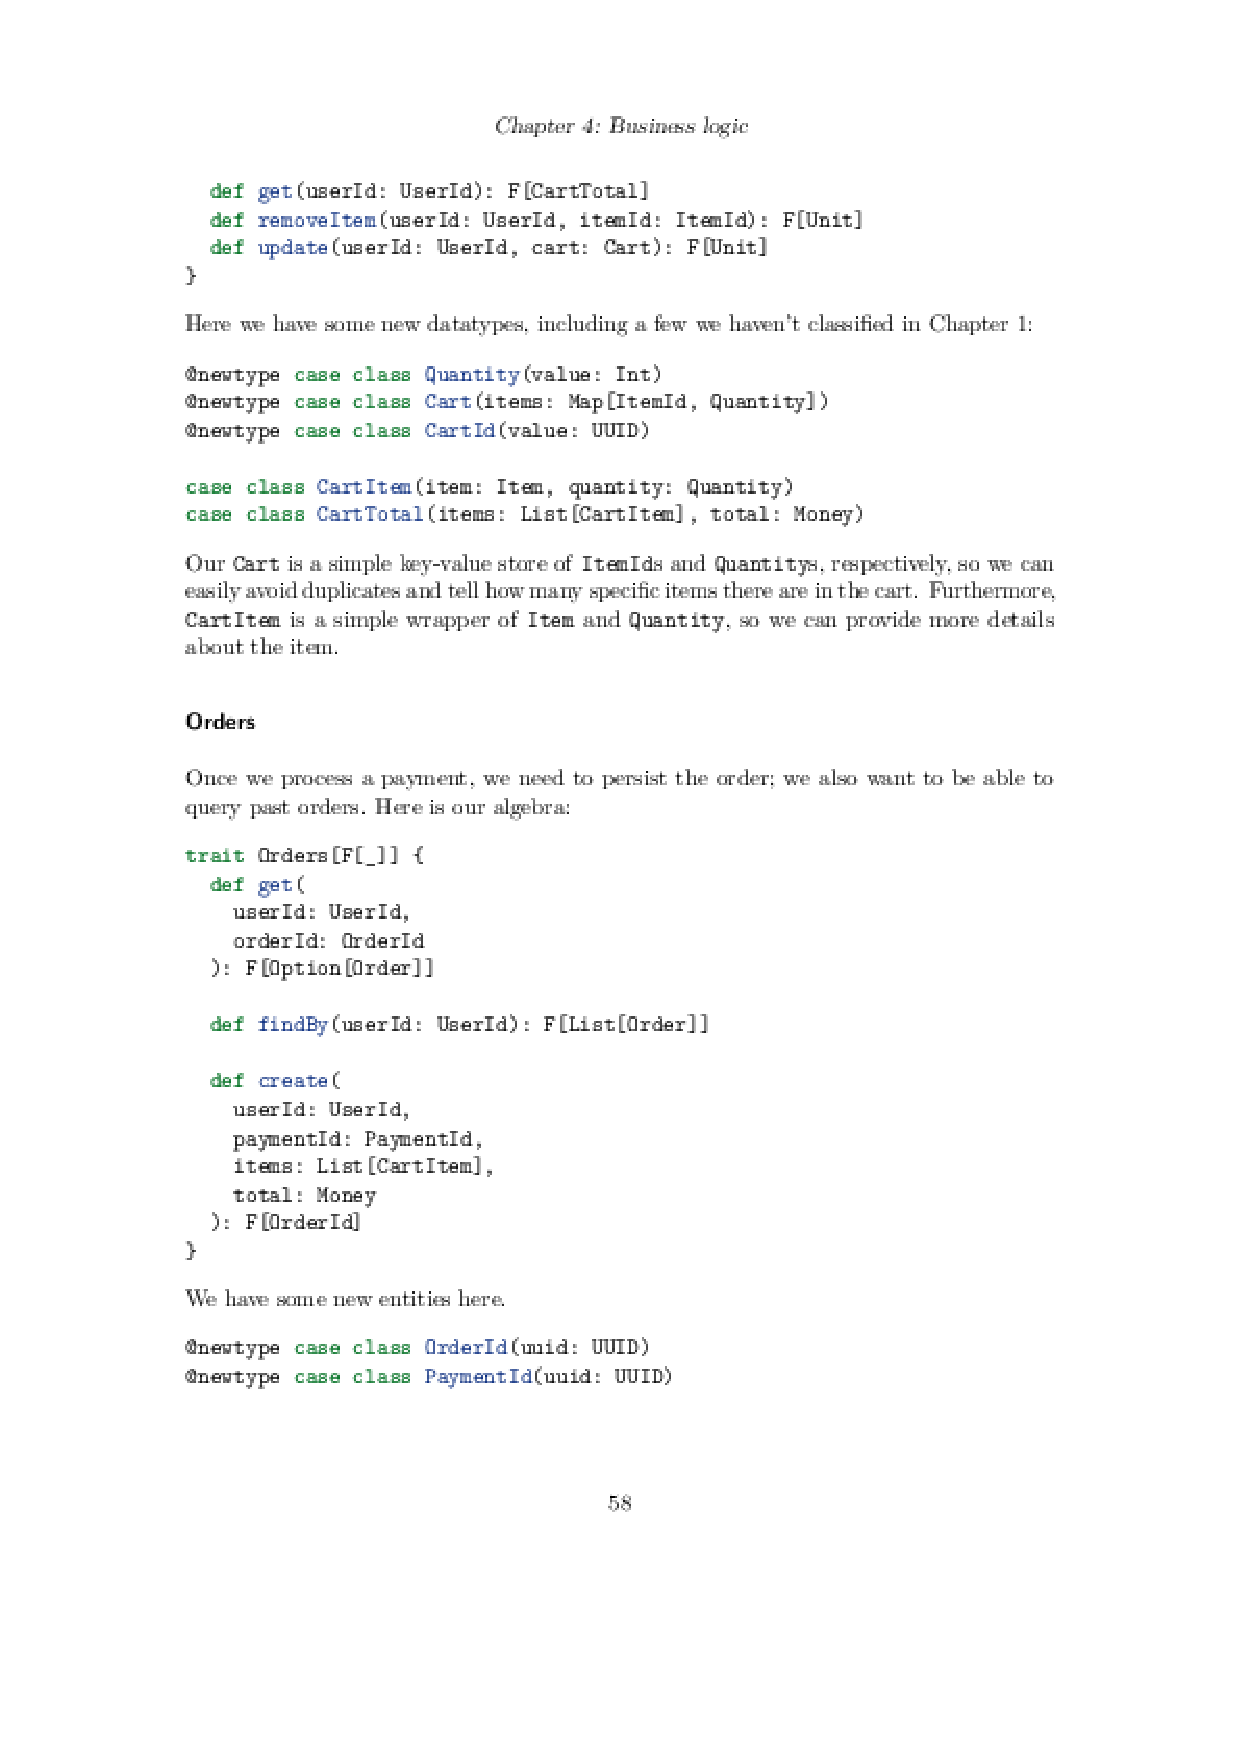
\includegraphics[height=2.51cm]{random-pages/random-pages-from-volpe-pdf-07}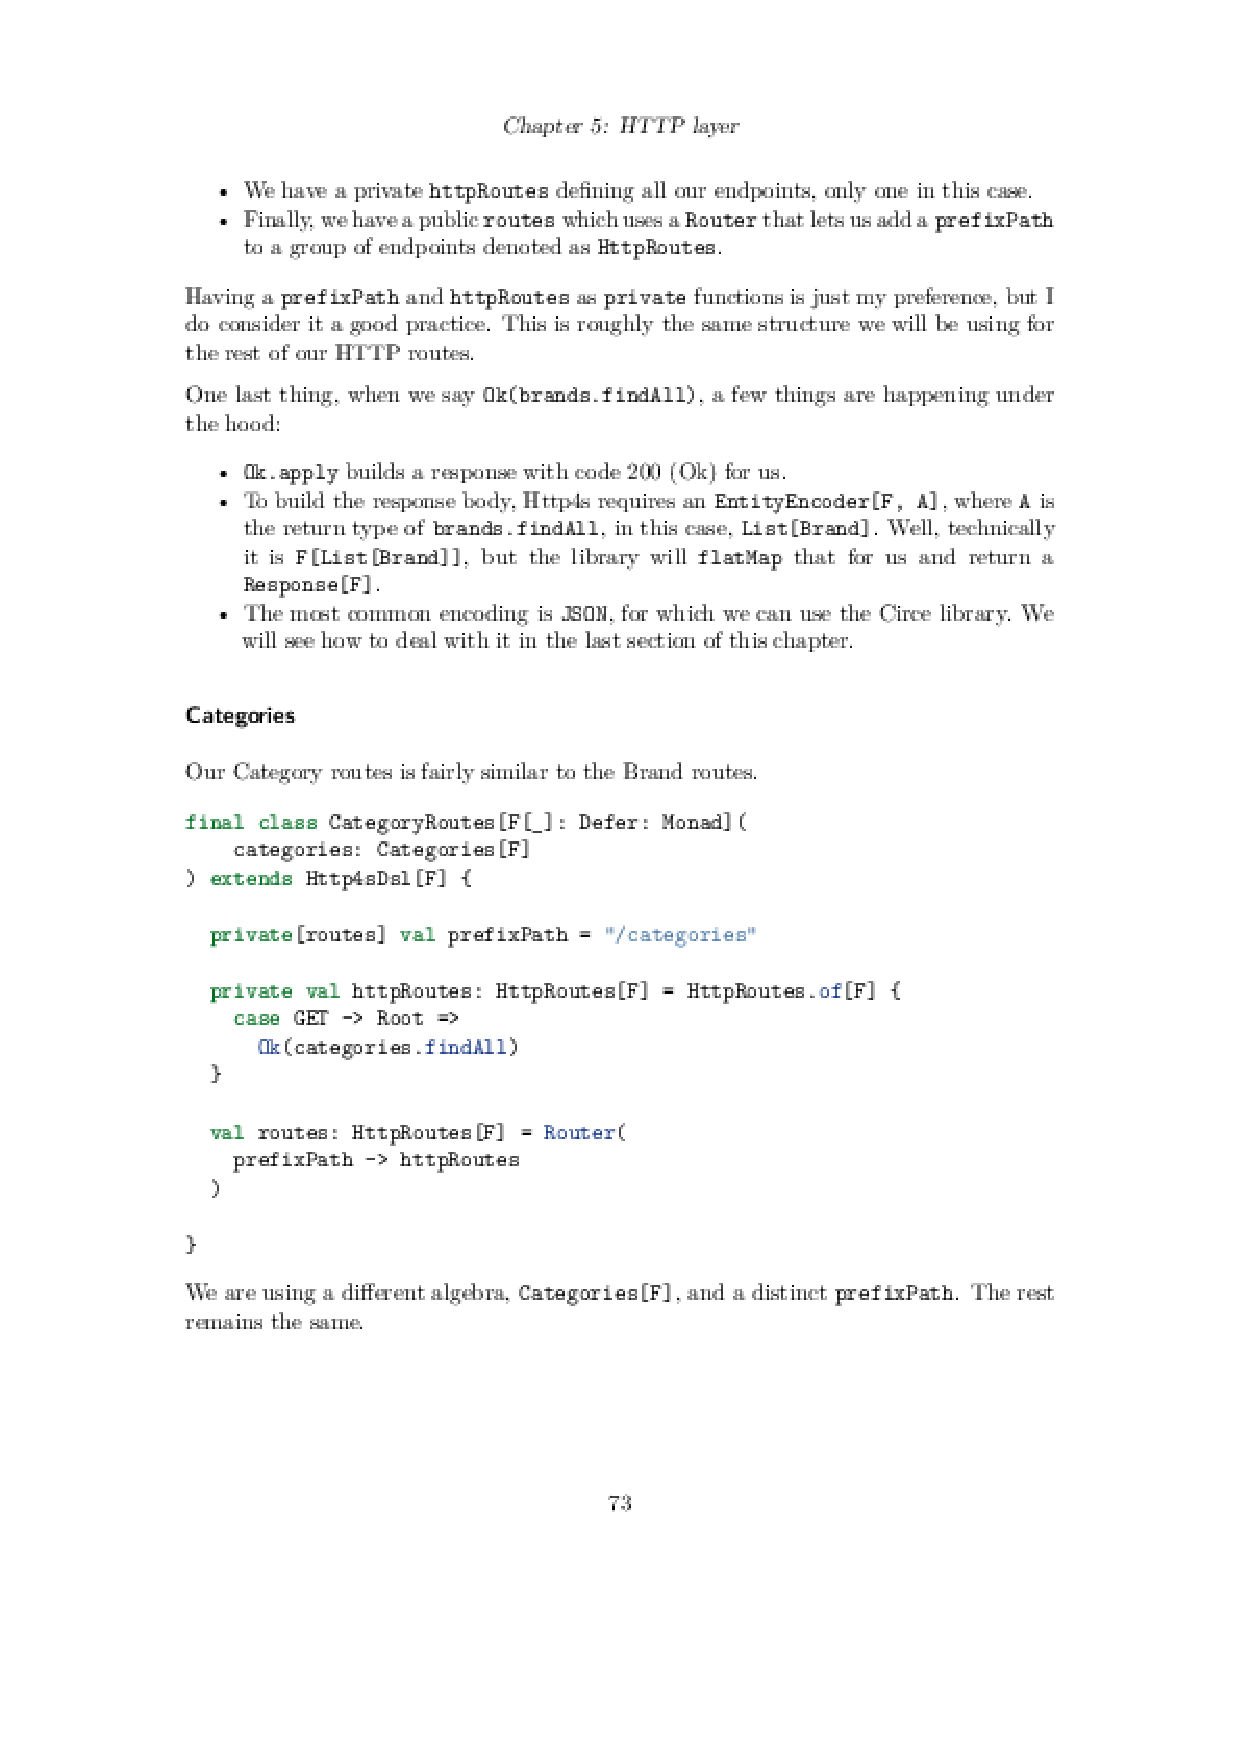
\includegraphics[height=2.51cm]{random-pages/random-pages-from-volpe-pdf-08}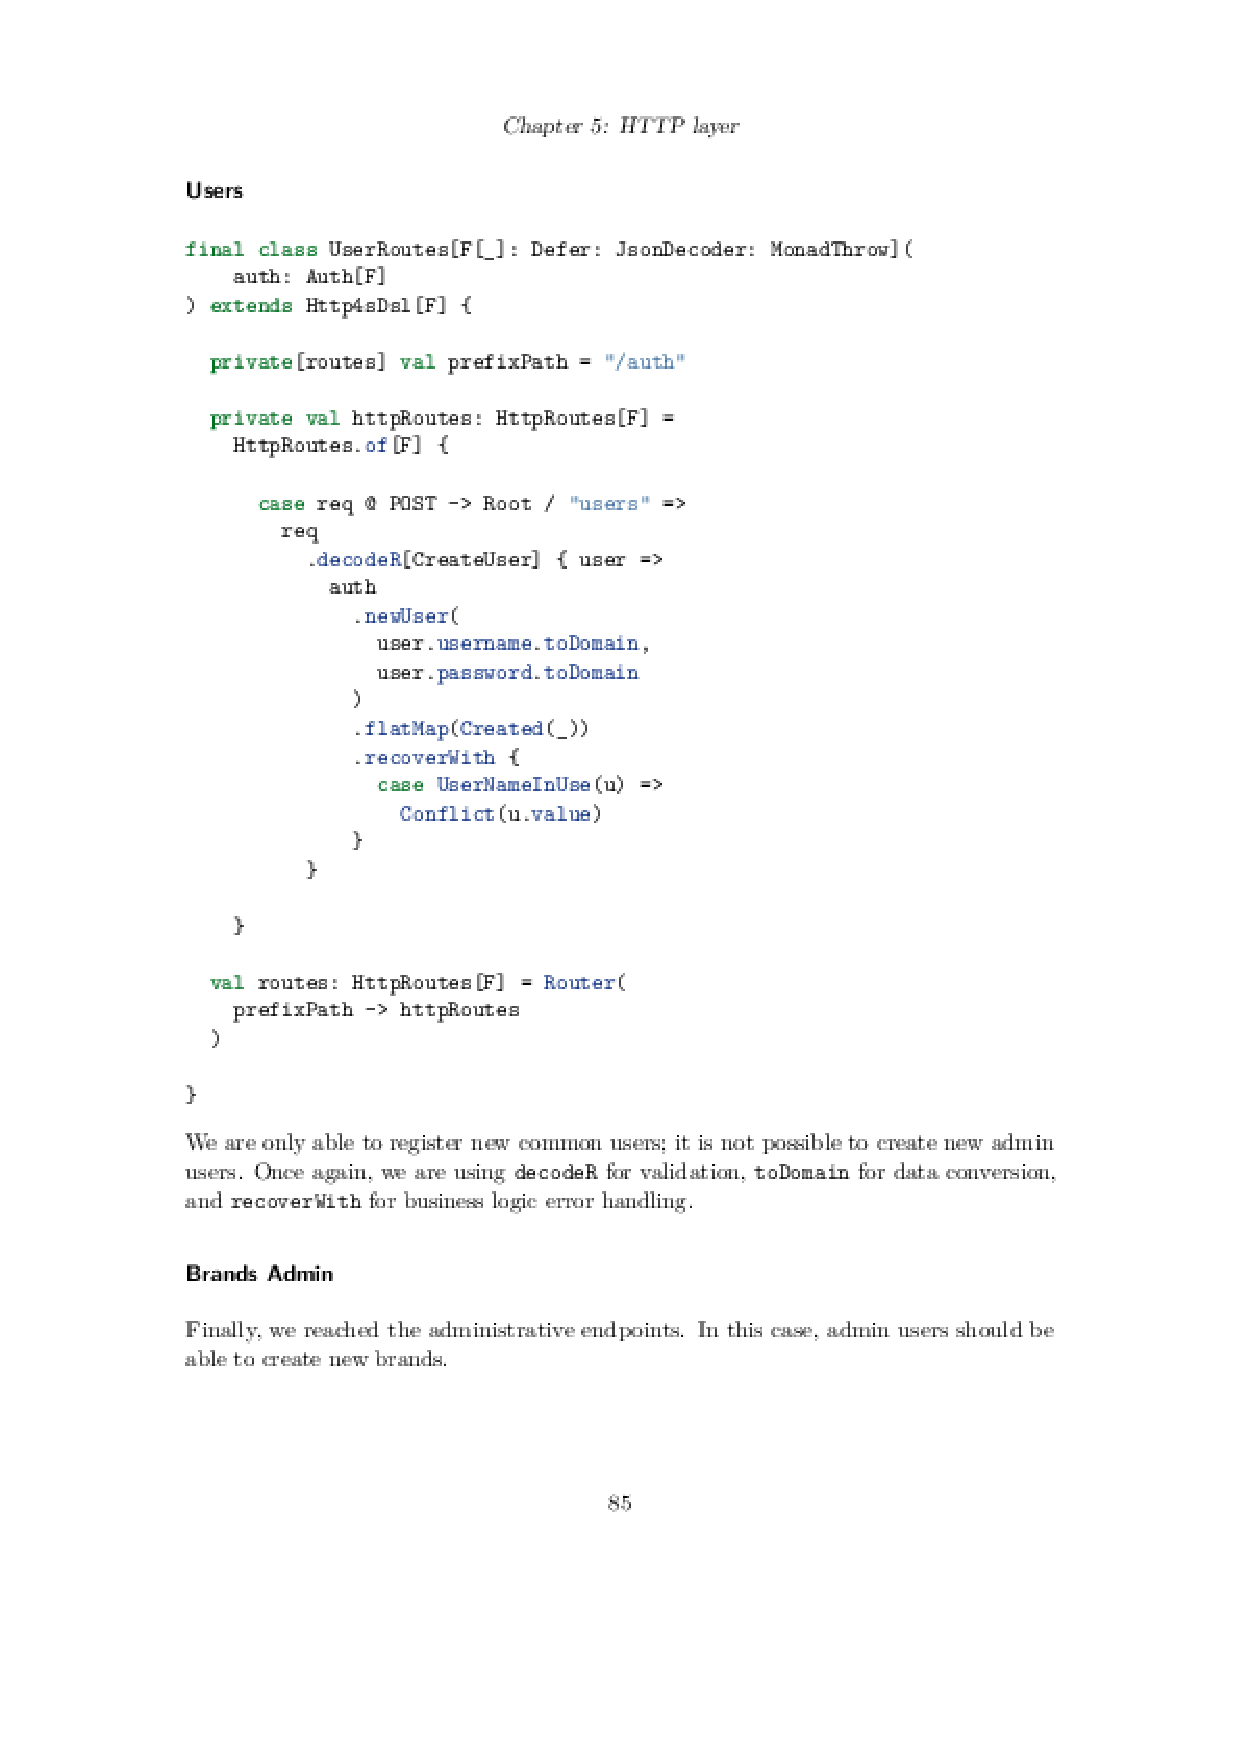
\includegraphics[height=2.51cm]{random-pages/random-pages-from-volpe-pdf-09}
\par\end{centering}
\begin{centering}
\textsf{``}Practical functional programming in Scala\textsf{''} by G.~Volpe (\texttt{\small{}\href{https://leanpub.com/pfp-scala}{https://leanpub.com/pfp-scala}})
\par\end{centering}
\begin{centering}
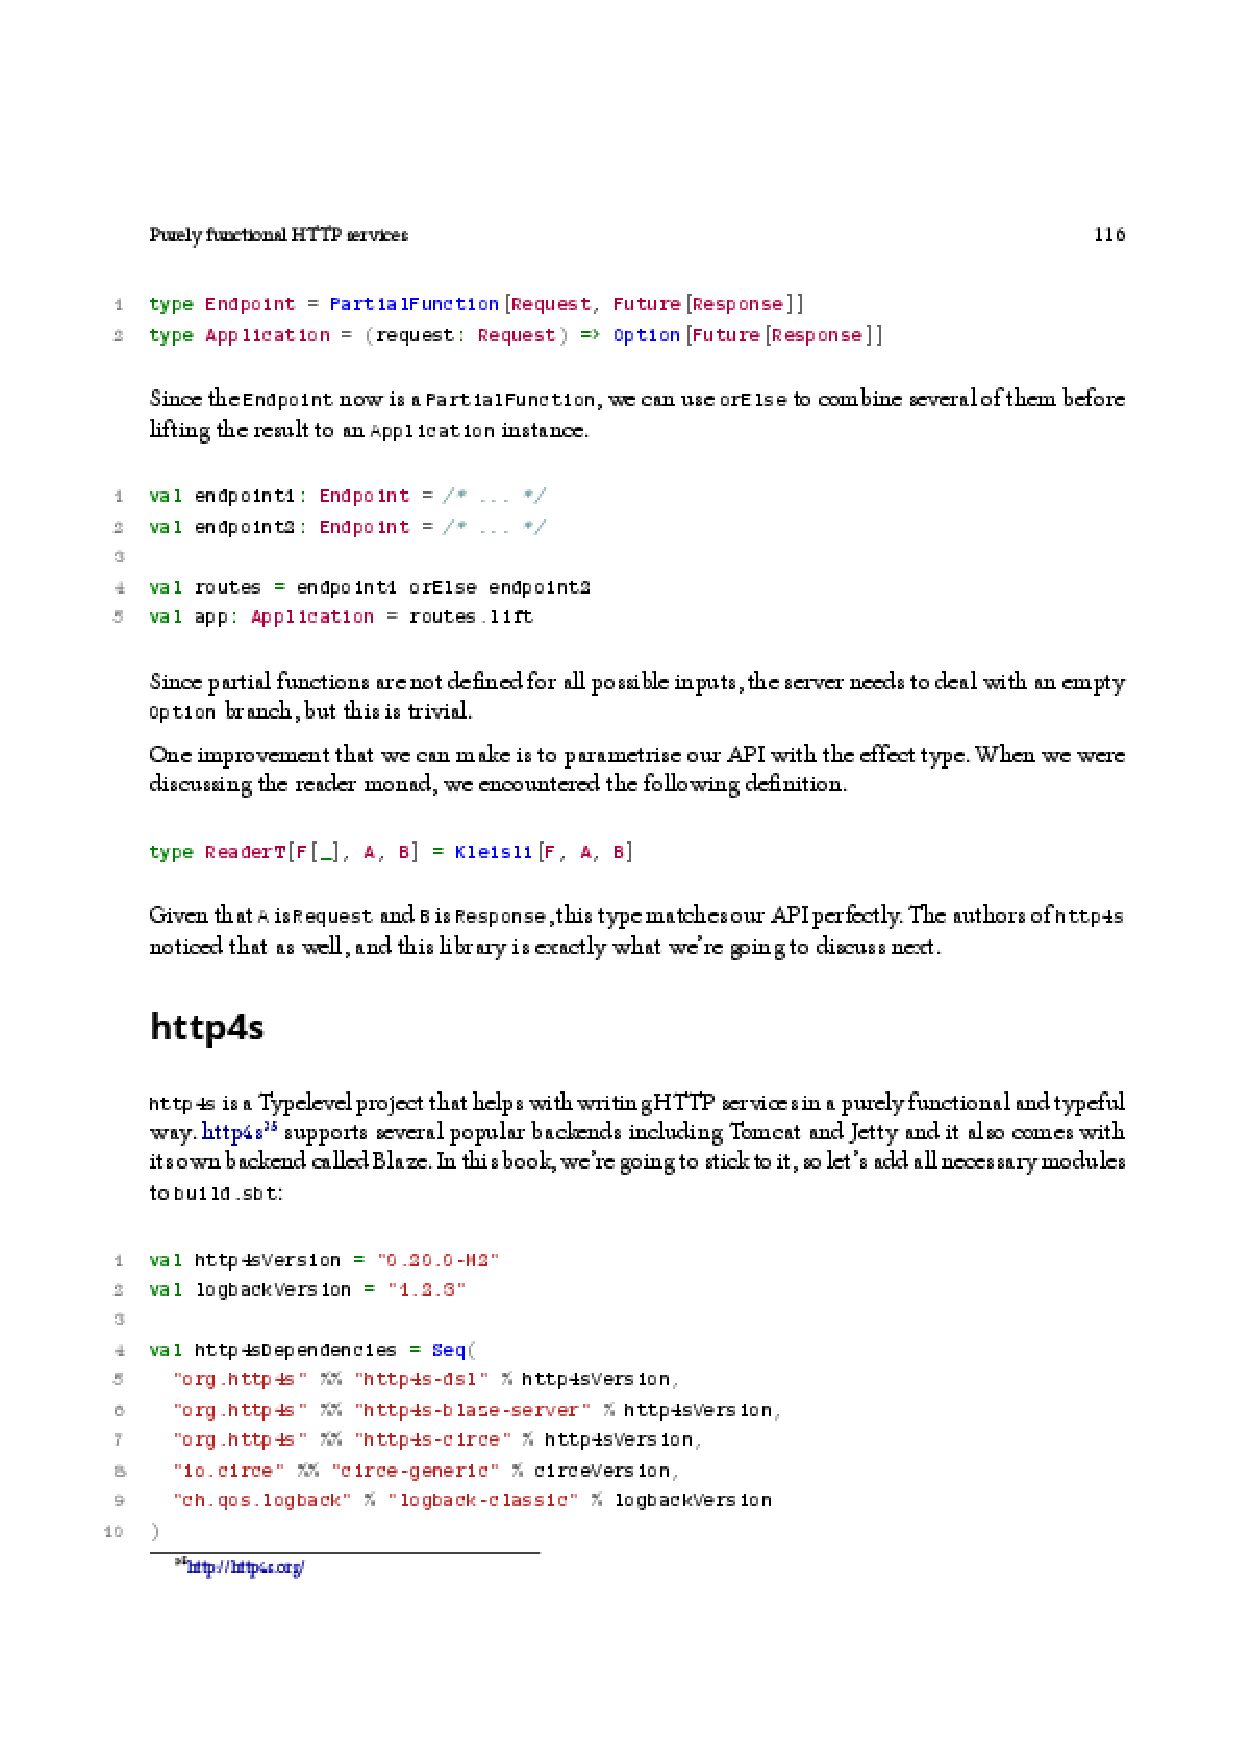
\includegraphics[height=2.51cm]{random-pages/random-pages-from-kalinin-pdf-01}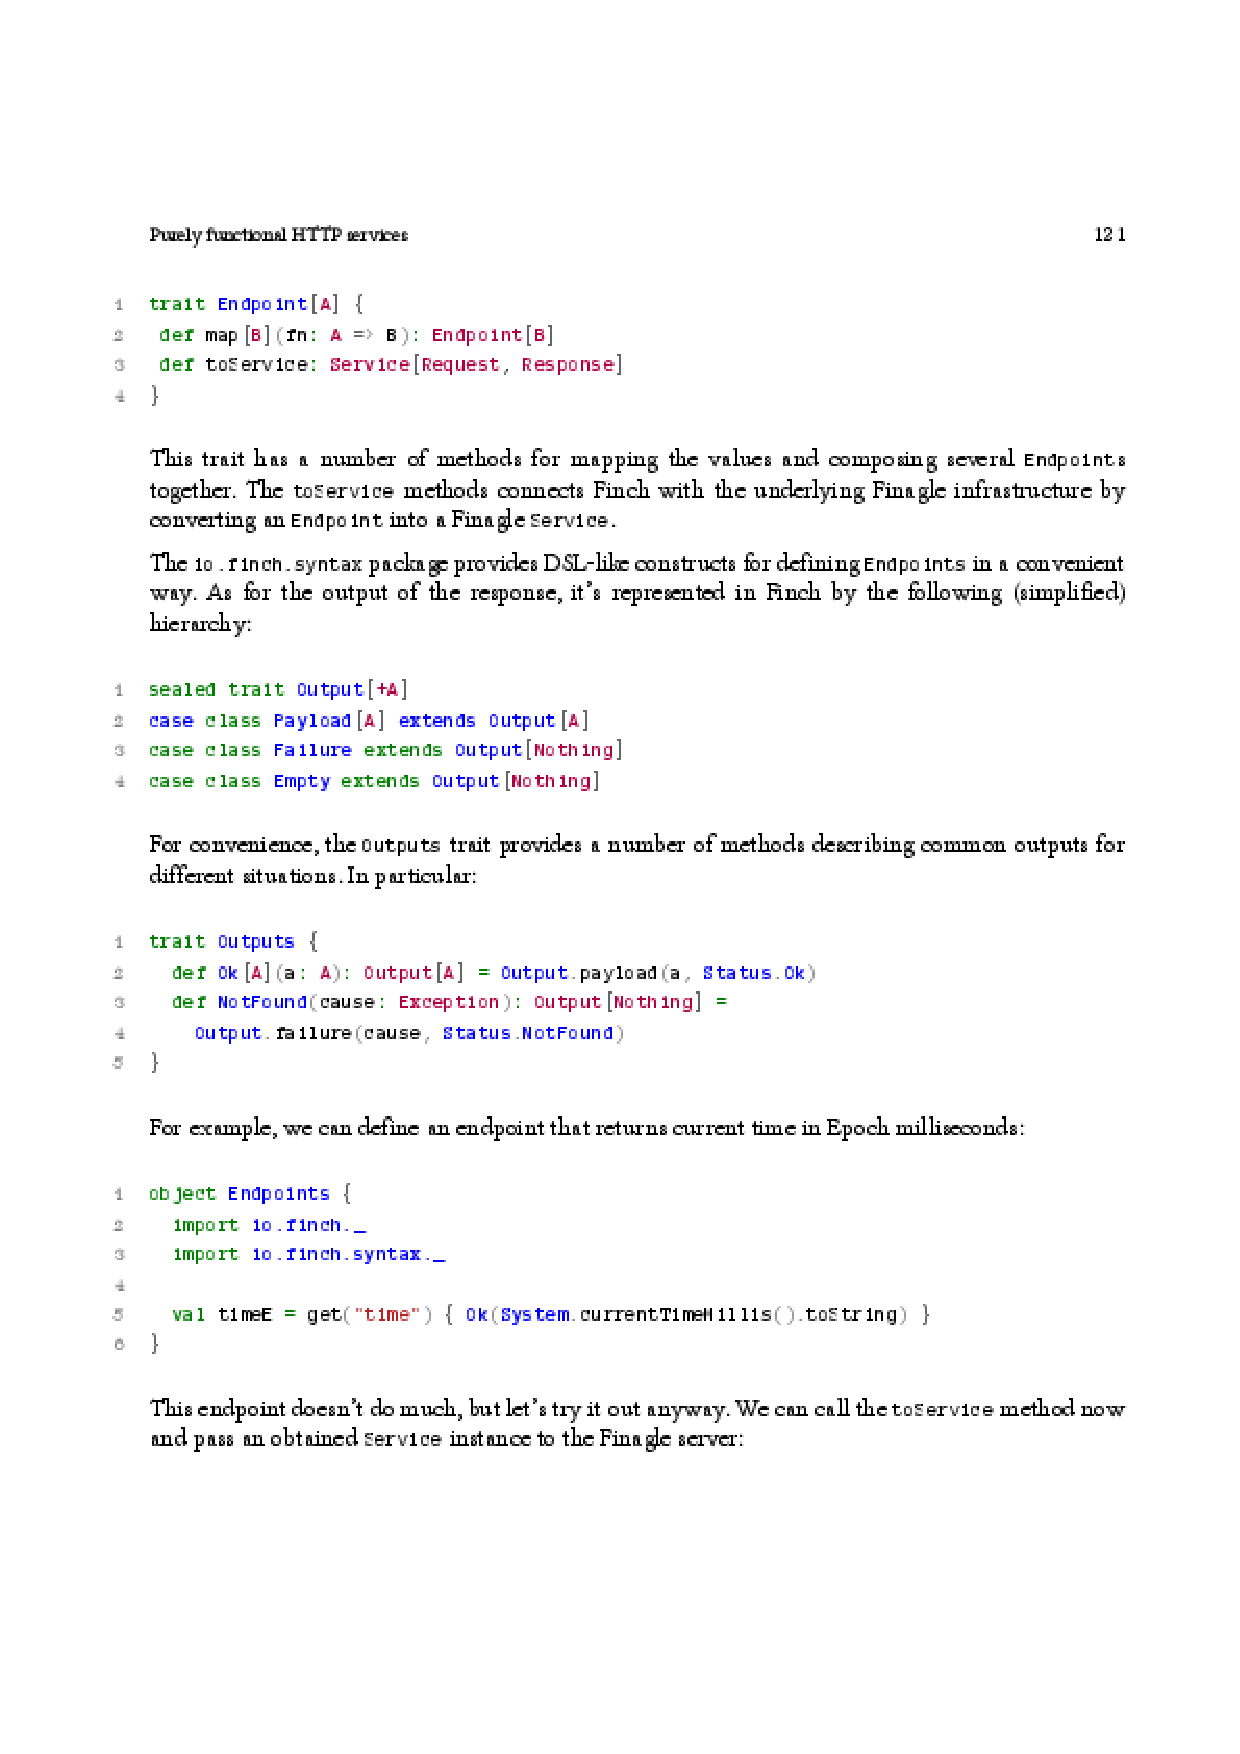
\includegraphics[height=2.51cm]{random-pages/random-pages-from-kalinin-pdf-02}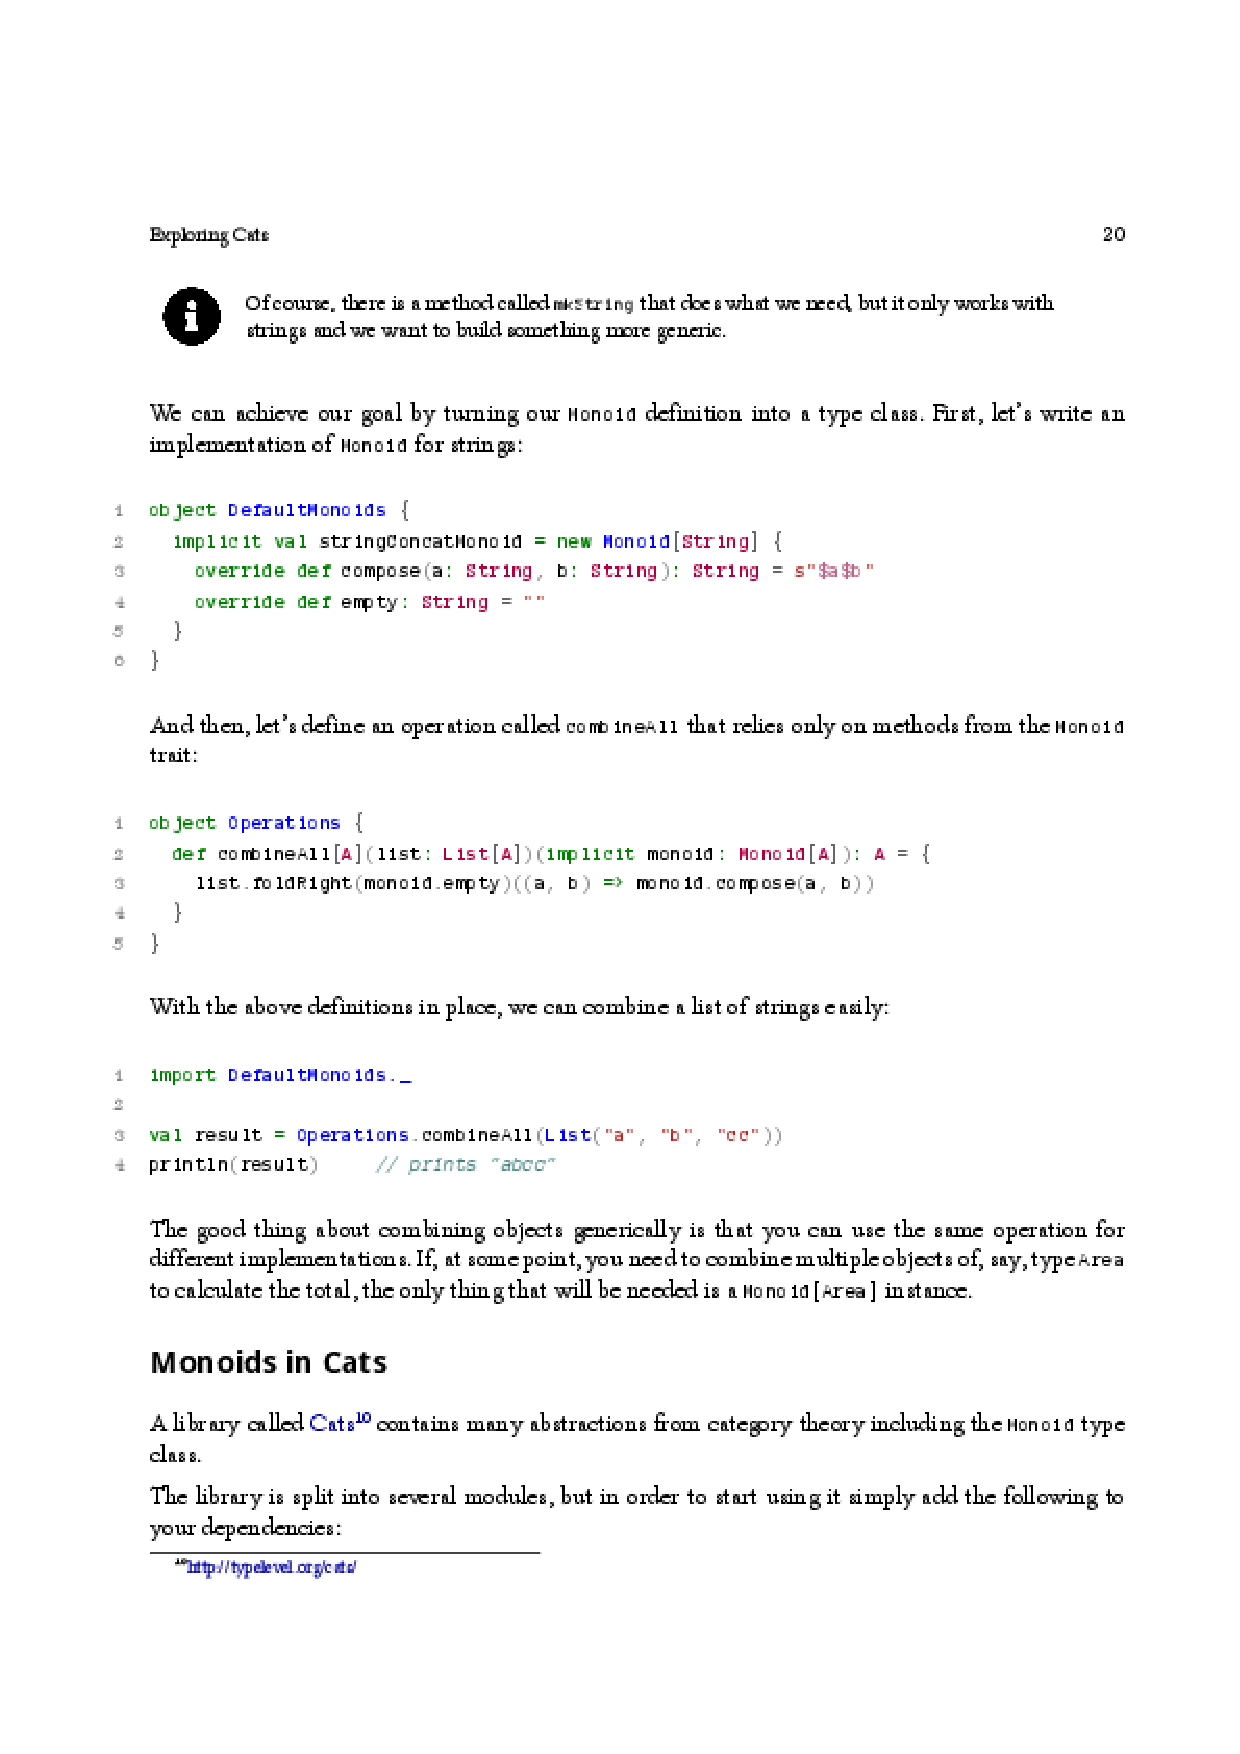
\includegraphics[height=2.51cm]{random-pages/random-pages-from-kalinin-pdf-03}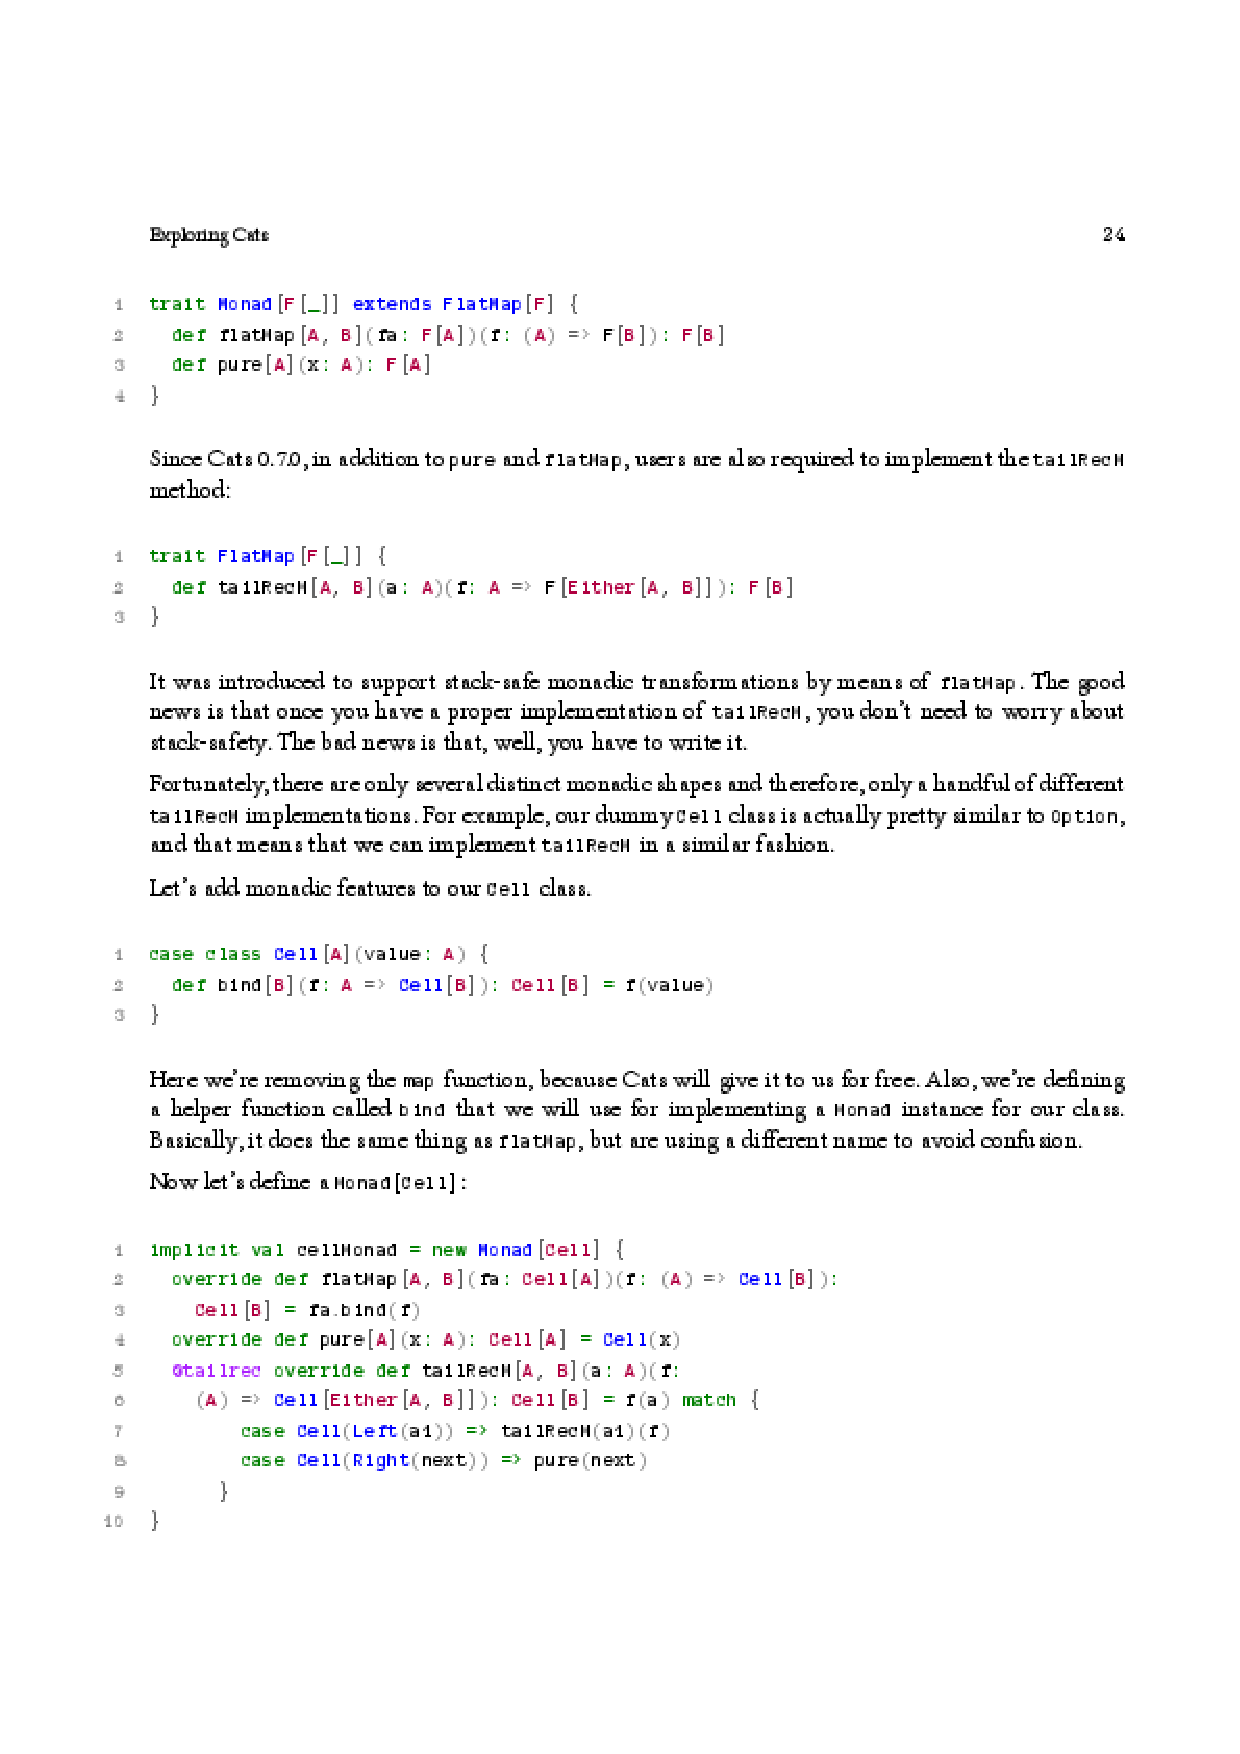
\includegraphics[height=2.51cm]{random-pages/random-pages-from-kalinin-pdf-04}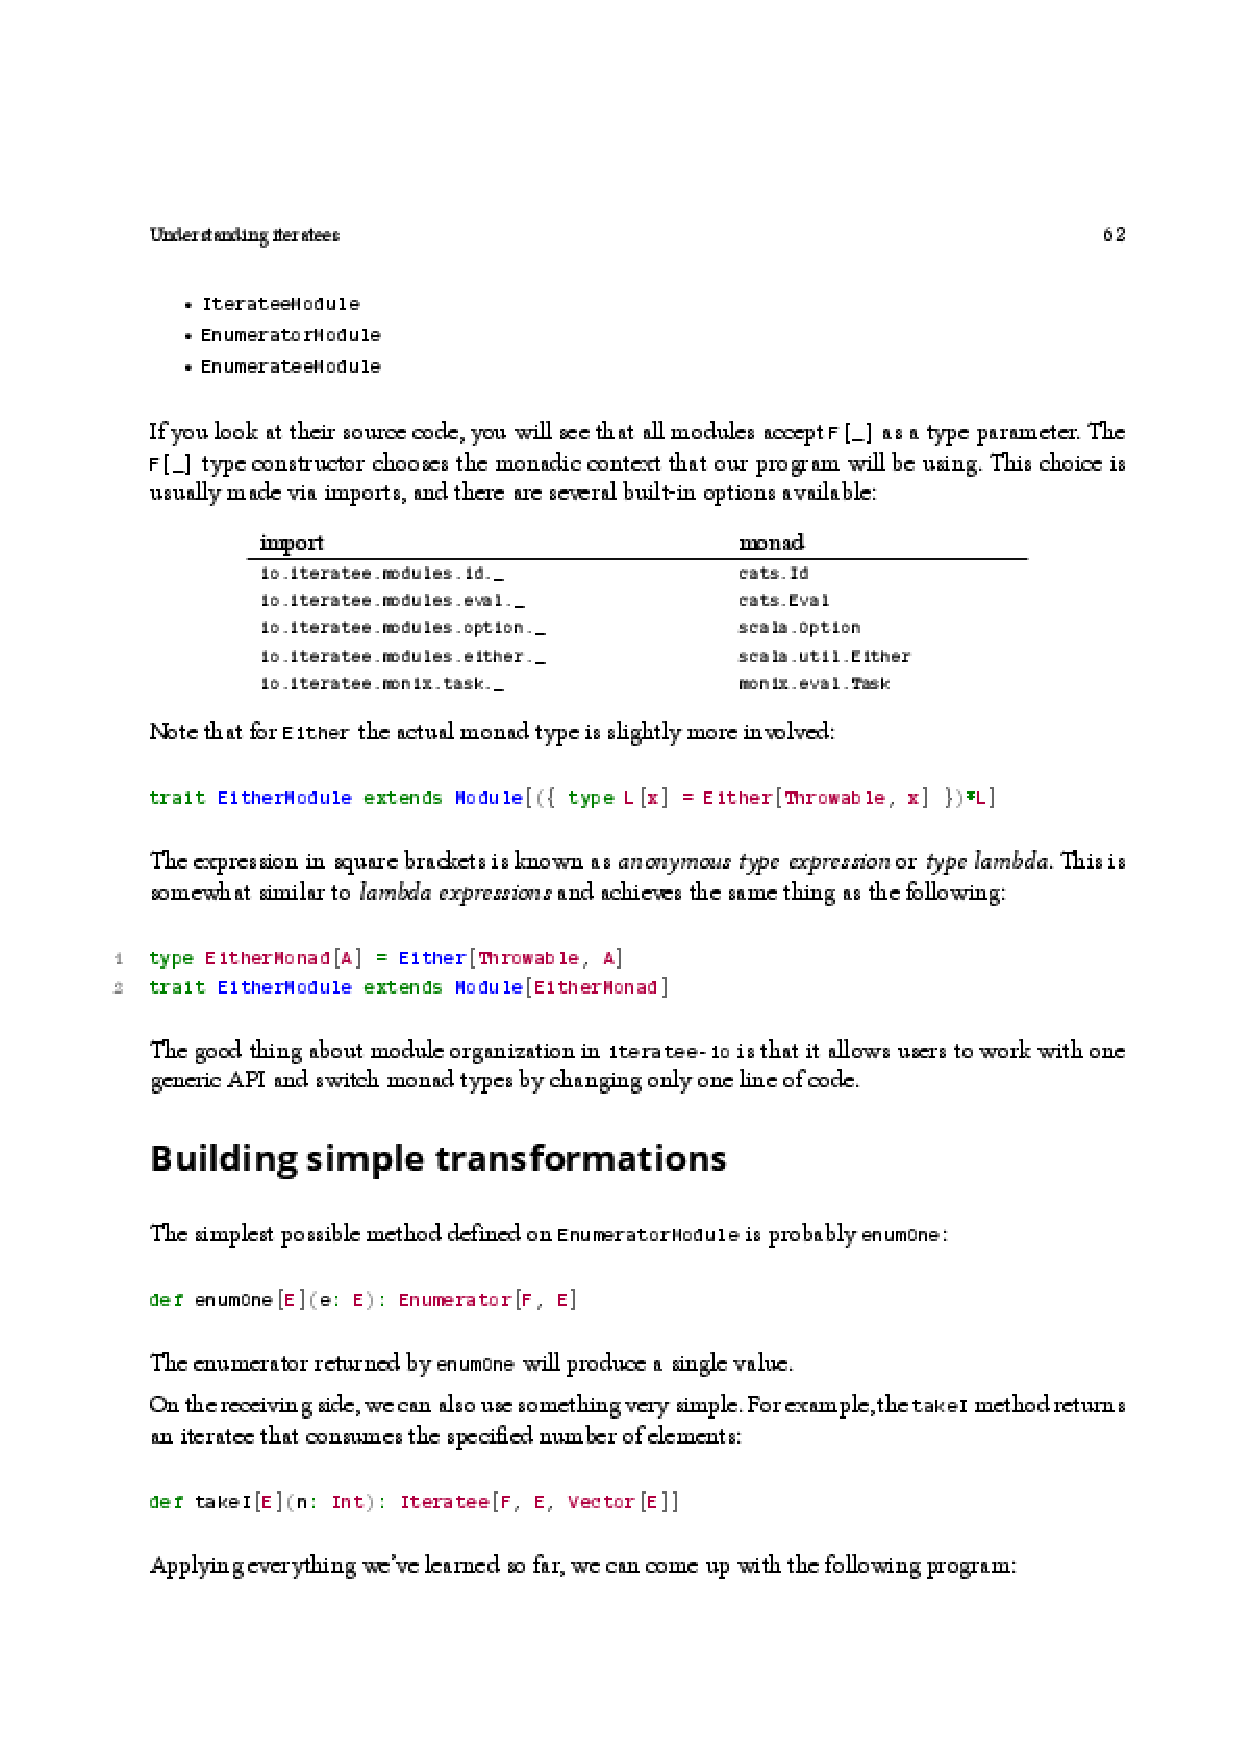
\includegraphics[height=2.51cm]{random-pages/random-pages-from-kalinin-pdf-06}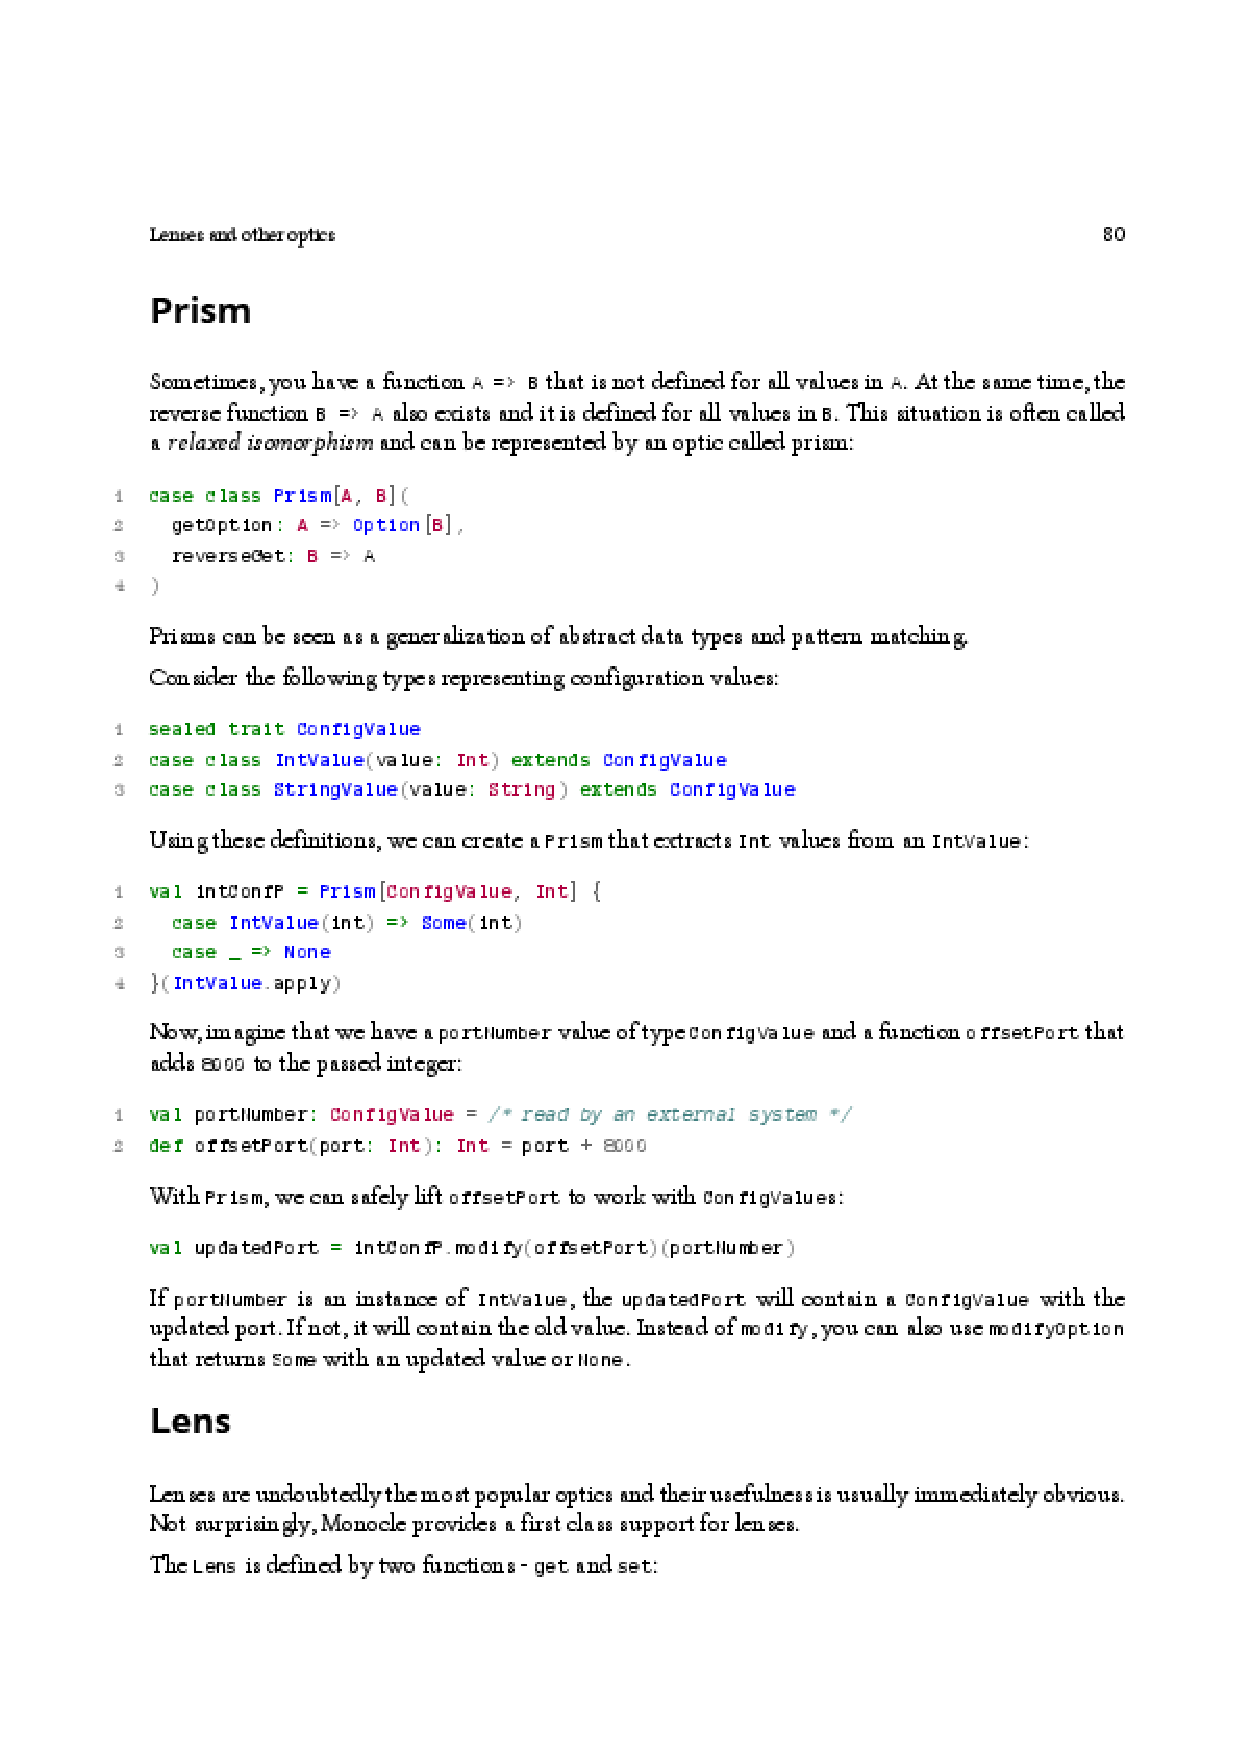
\includegraphics[height=2.51cm]{random-pages/random-pages-from-kalinin-pdf-07}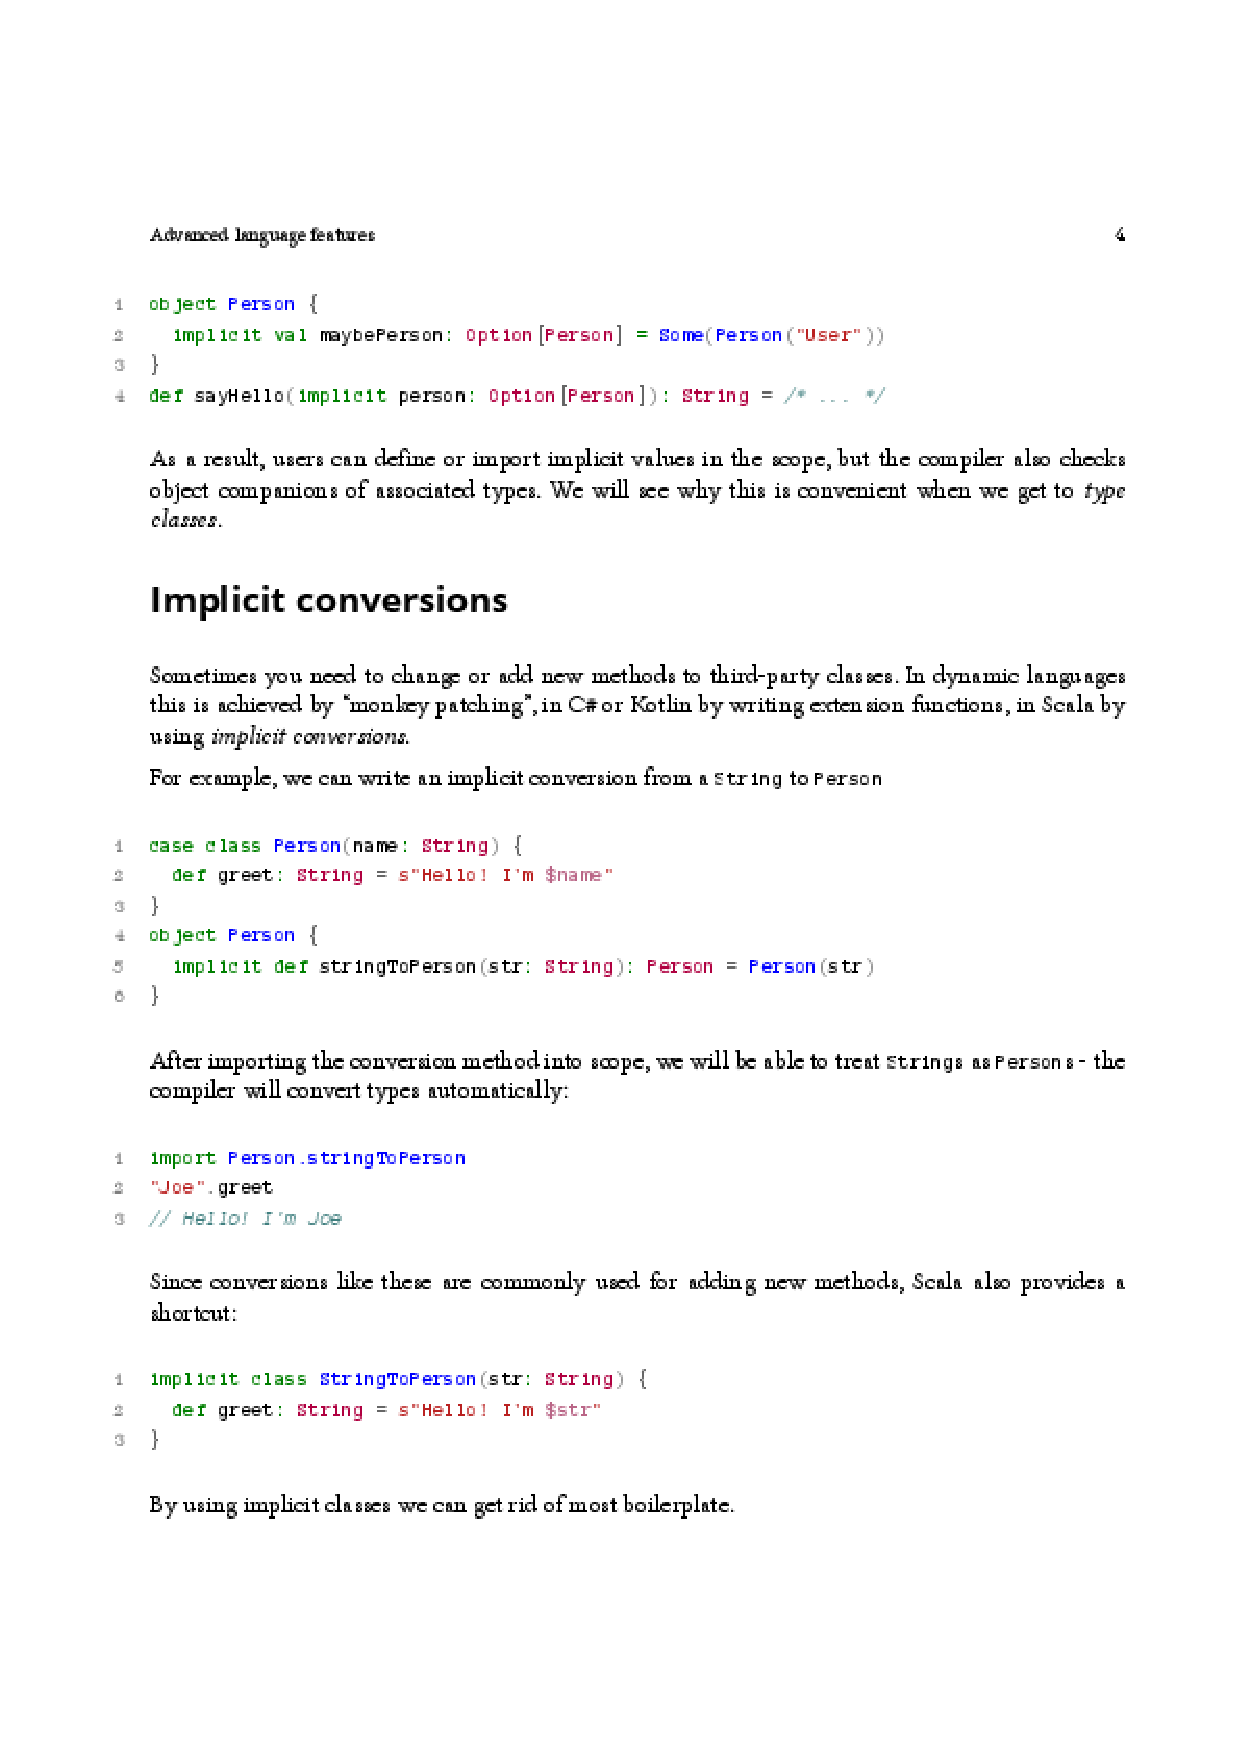
\includegraphics[height=2.51cm]{random-pages/random-pages-from-kalinin-pdf-08}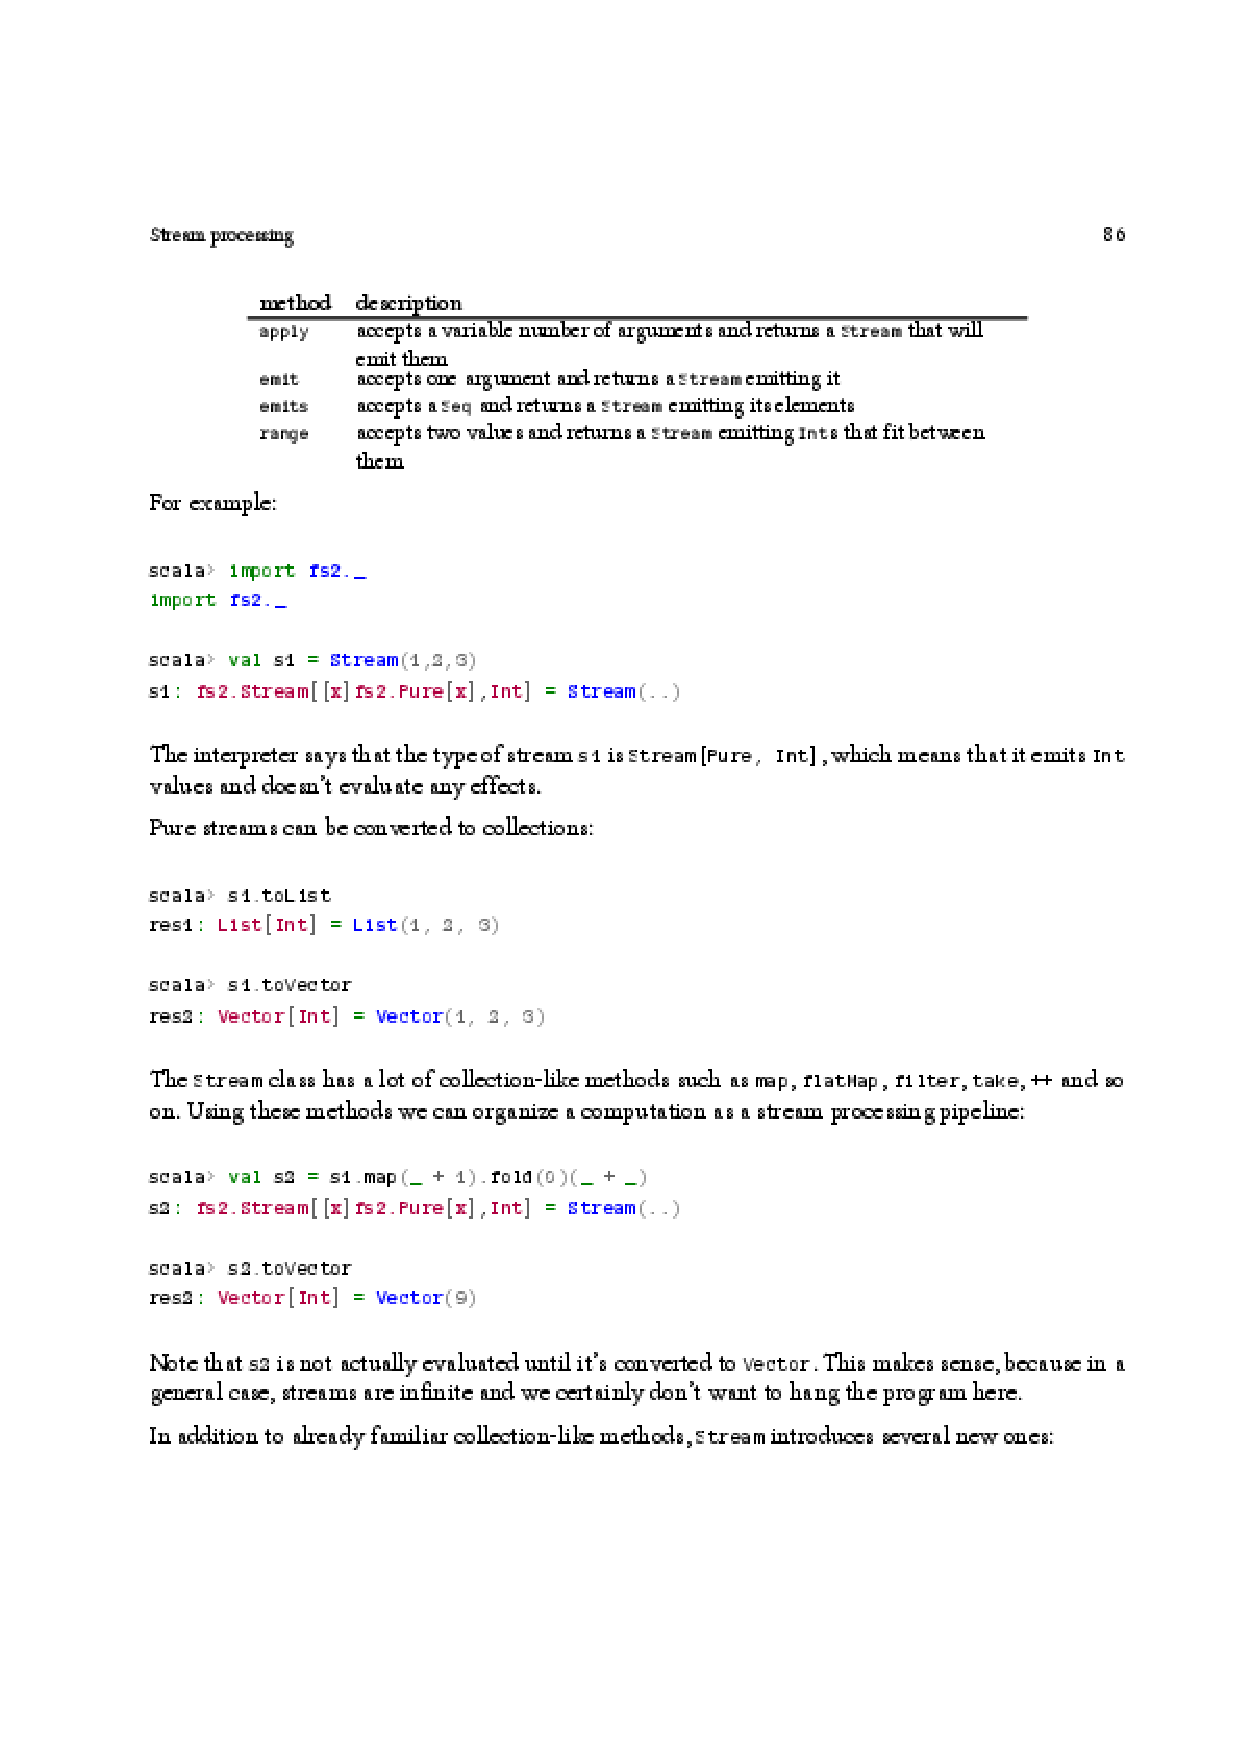
\includegraphics[height=2.51cm]{random-pages/random-pages-from-kalinin-pdf-09}
\par\end{centering}
\begin{centering}
\textsf{``}Mastering advanced Scala\textsf{''} by D.~Kalinin (\texttt{\small{}\href{https://leanpub.com/mastering-advanced-scala}{https://leanpub.com/mastering-advanced-scala}})
\par\end{centering}
\caption{Randomly chosen pages from books on Scala programming.\label{fig:Randomly-chosen-pages-1}}
\end{figure}

\begin{figure}
\begin{centering}
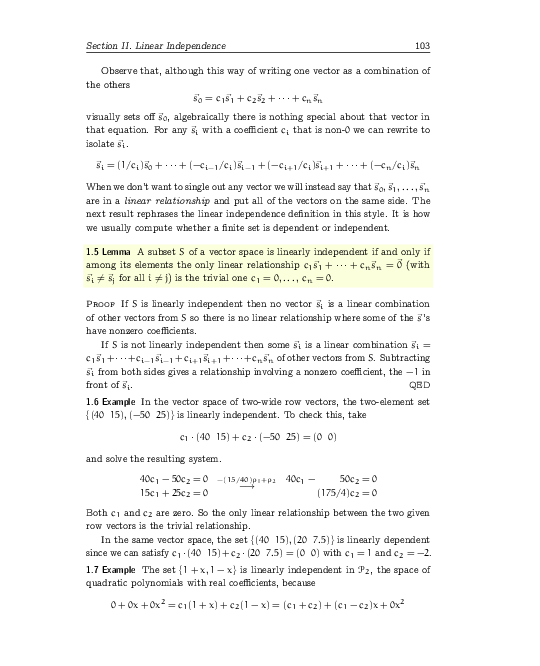
\includegraphics[height=2.51cm]{random-pages/random-pages-from-hefferon-pdf-00}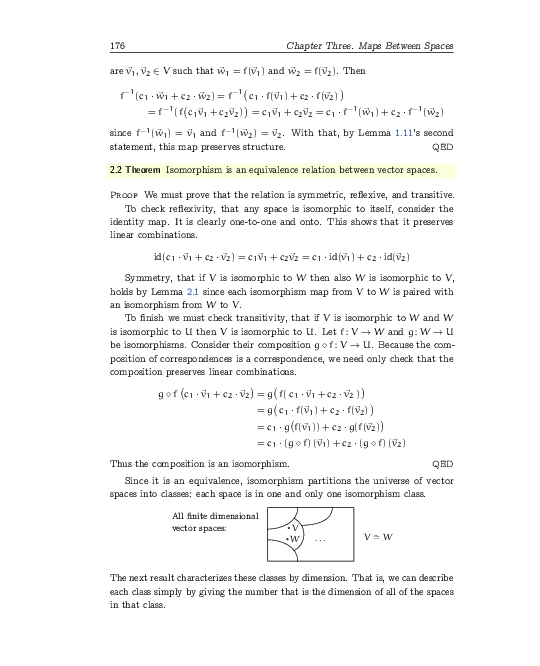
\includegraphics[height=2.51cm]{random-pages/random-pages-from-hefferon-pdf-01}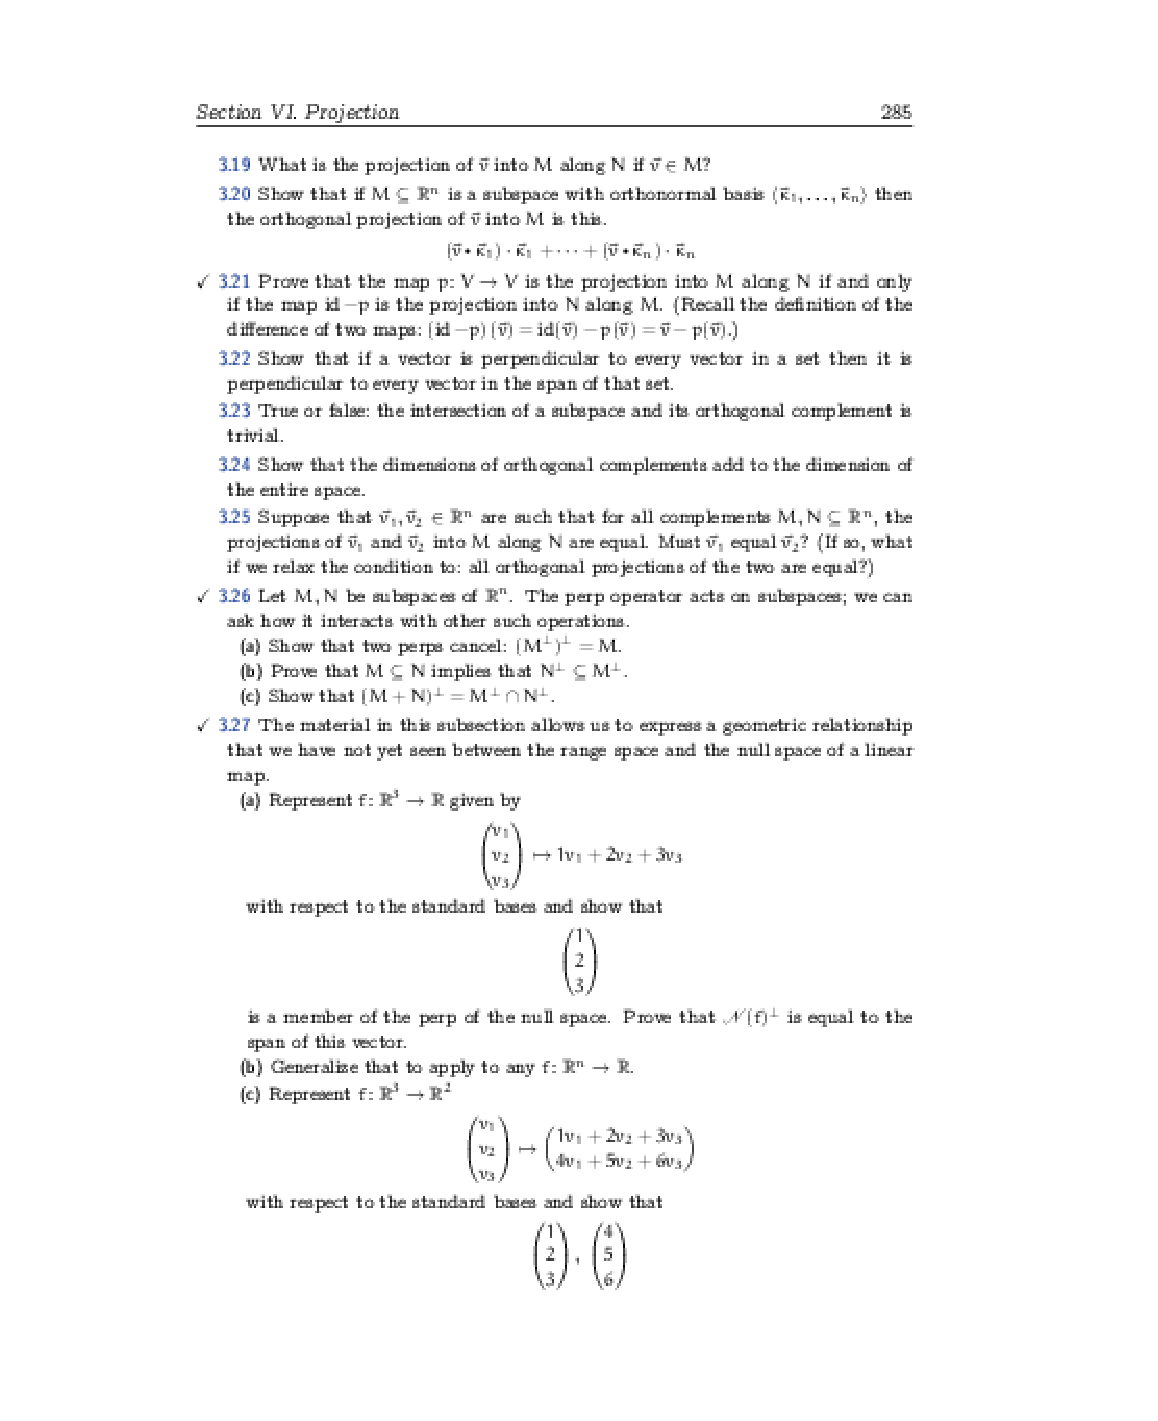
\includegraphics[height=2.51cm]{random-pages/random-pages-from-hefferon-pdf-02}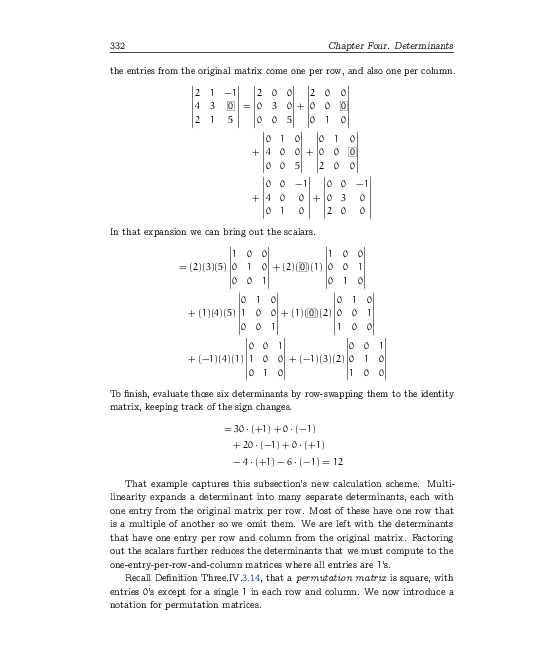
\includegraphics[height=2.51cm]{random-pages/random-pages-from-hefferon-pdf-03}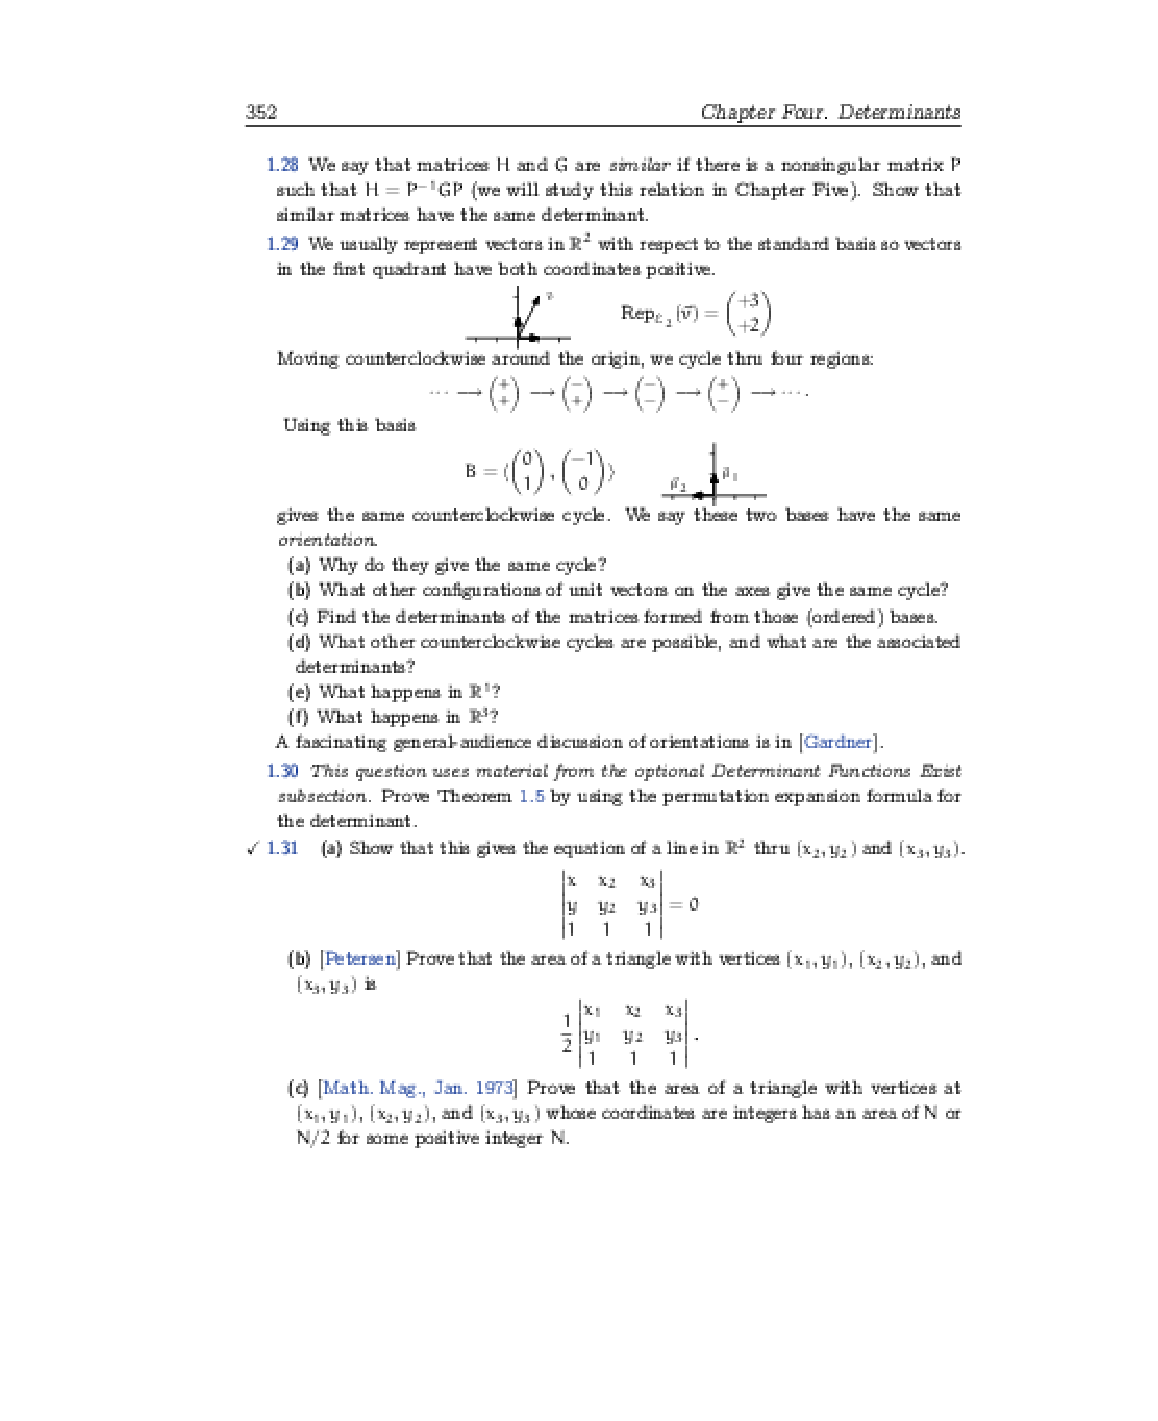
\includegraphics[height=2.51cm]{random-pages/random-pages-from-hefferon-pdf-04}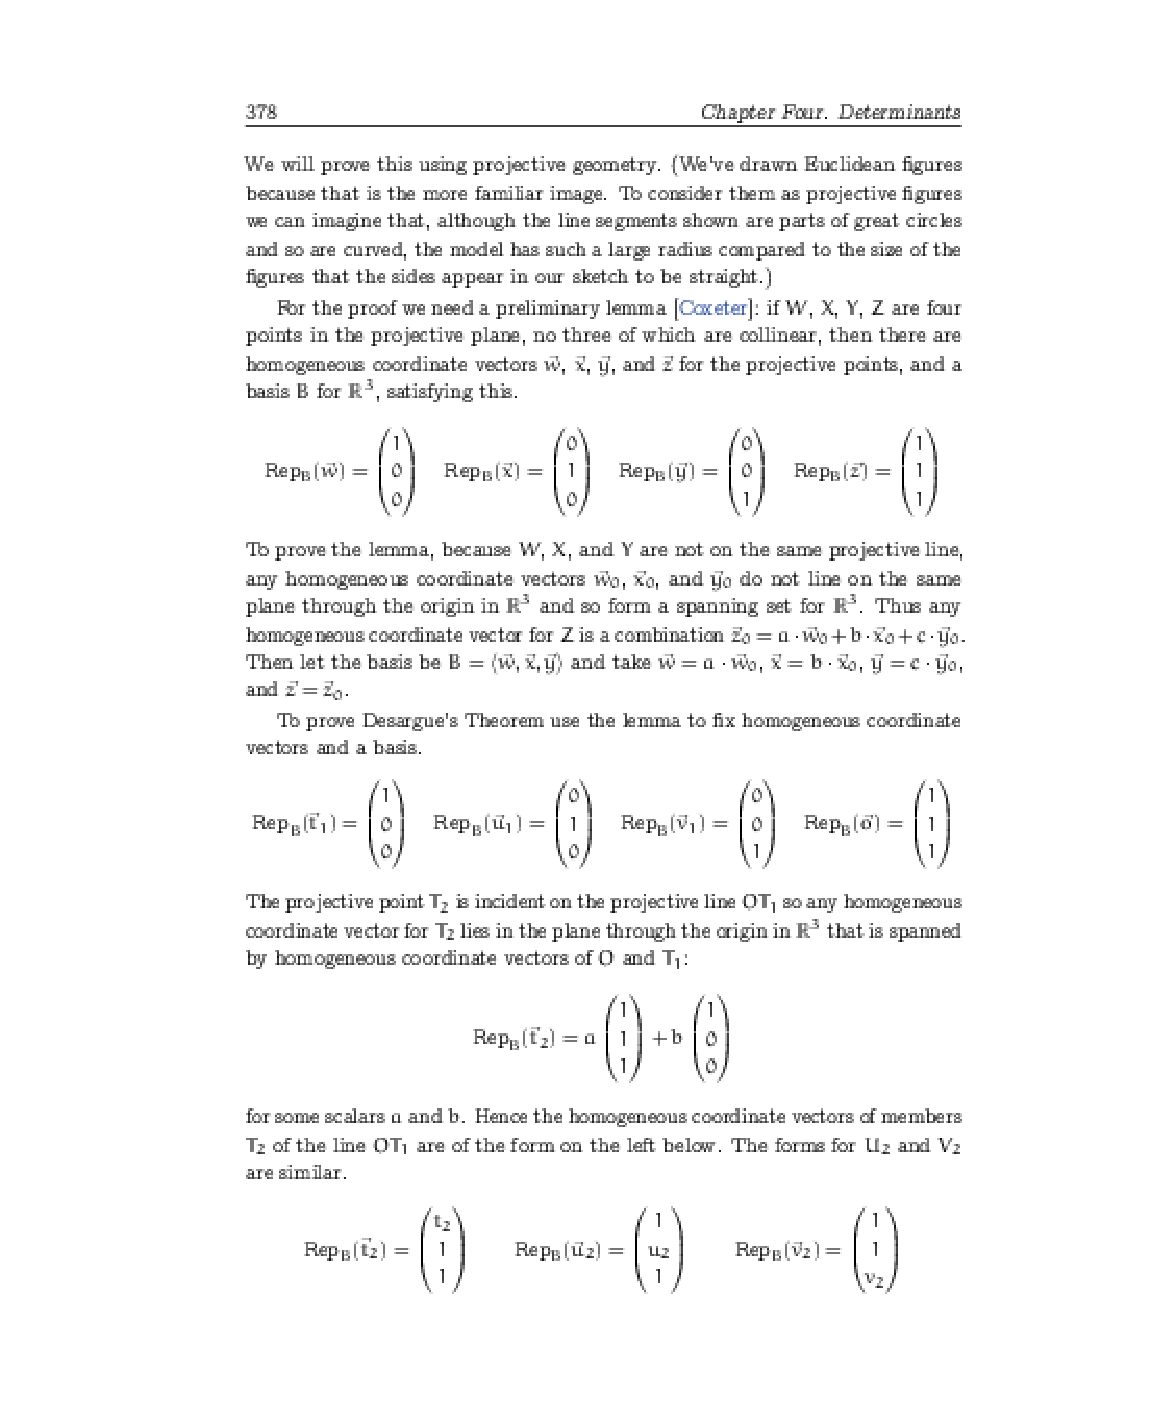
\includegraphics[height=2.51cm]{random-pages/random-pages-from-hefferon-pdf-05}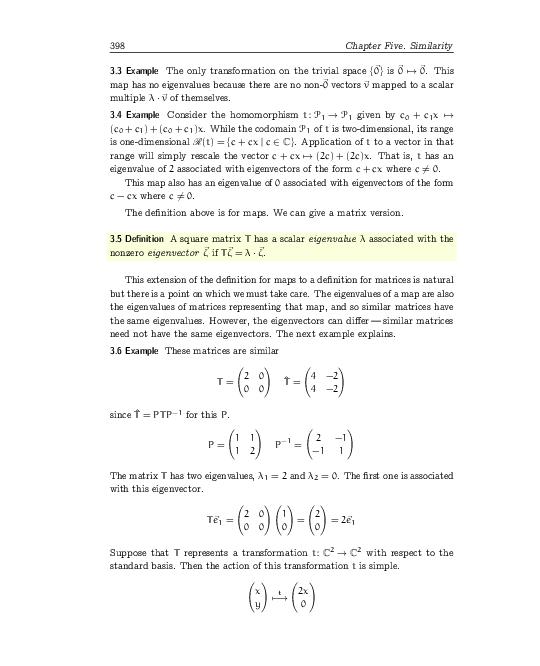
\includegraphics[height=2.51cm]{random-pages/random-pages-from-hefferon-pdf-06}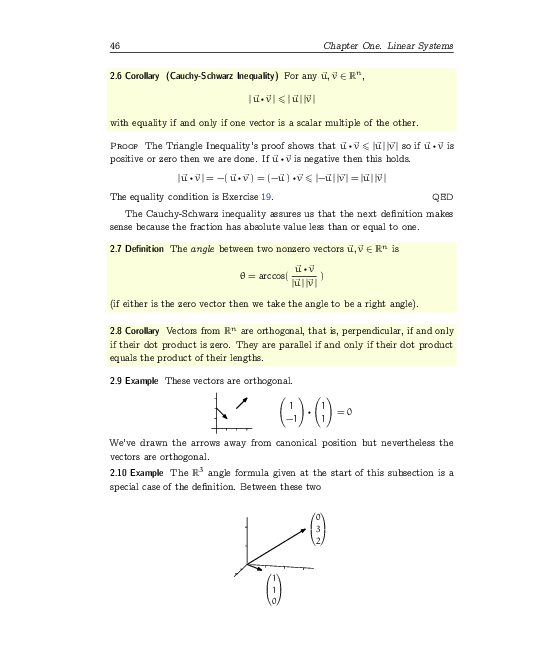
\includegraphics[height=2.51cm]{random-pages/random-pages-from-hefferon-pdf-07}
\par\end{centering}
\begin{centering}
\textsf{``}Linear algebra\textsf{''} by J.~Hefferon (\texttt{\small{}\href{http://joshua.smcvt.edu/linearalgebra/}{http://joshua.smcvt.edu/linearalgebra/}})
\par\end{centering}
\begin{centering}
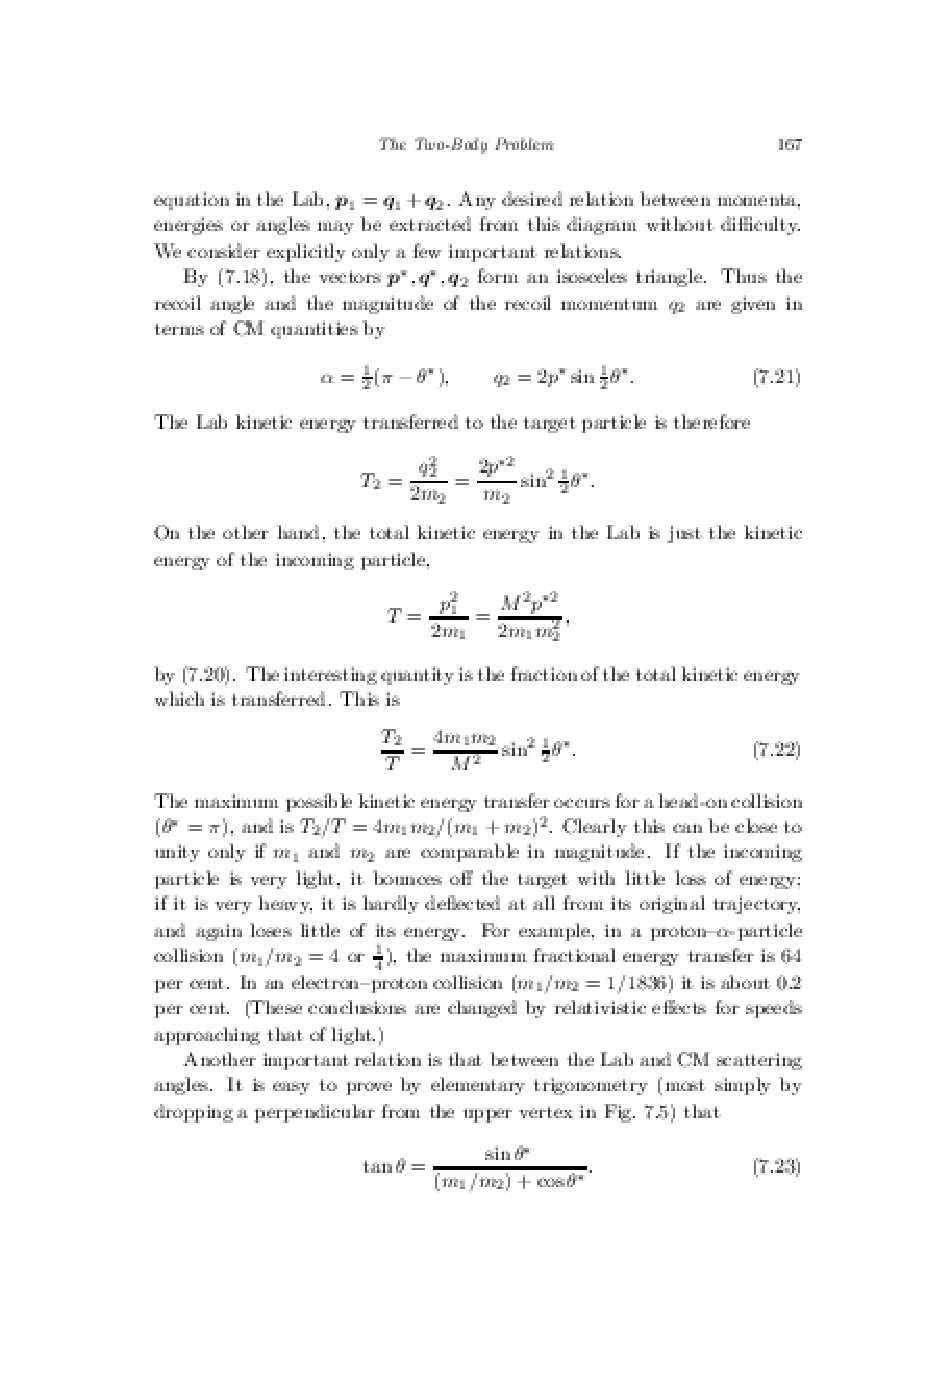
\includegraphics[height=2.51cm]{random-pages/random-pages-from-kibble-pdf-00}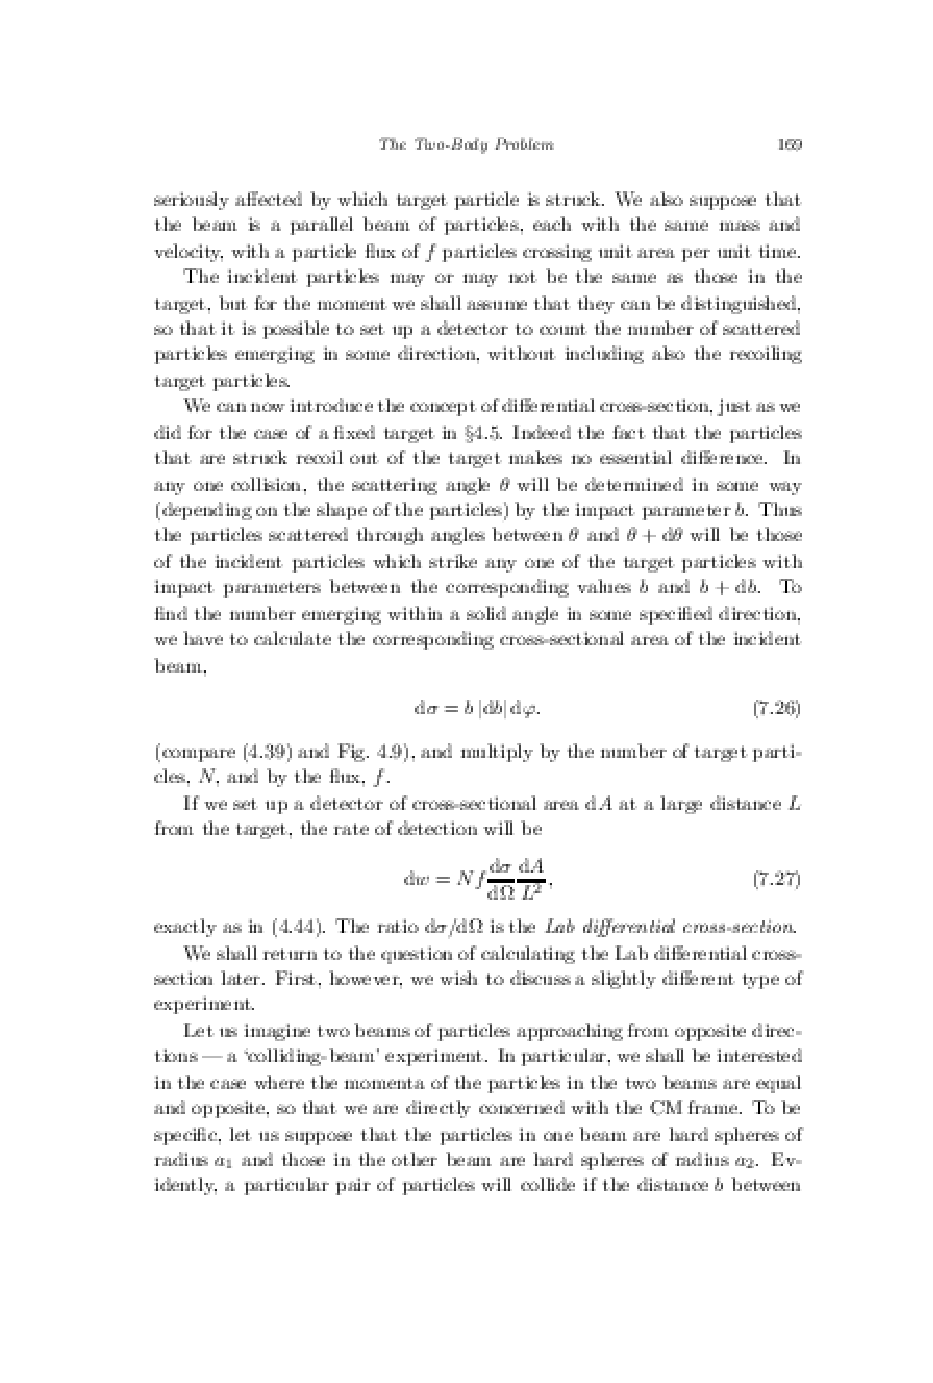
\includegraphics[height=2.51cm]{random-pages/random-pages-from-kibble-pdf-01}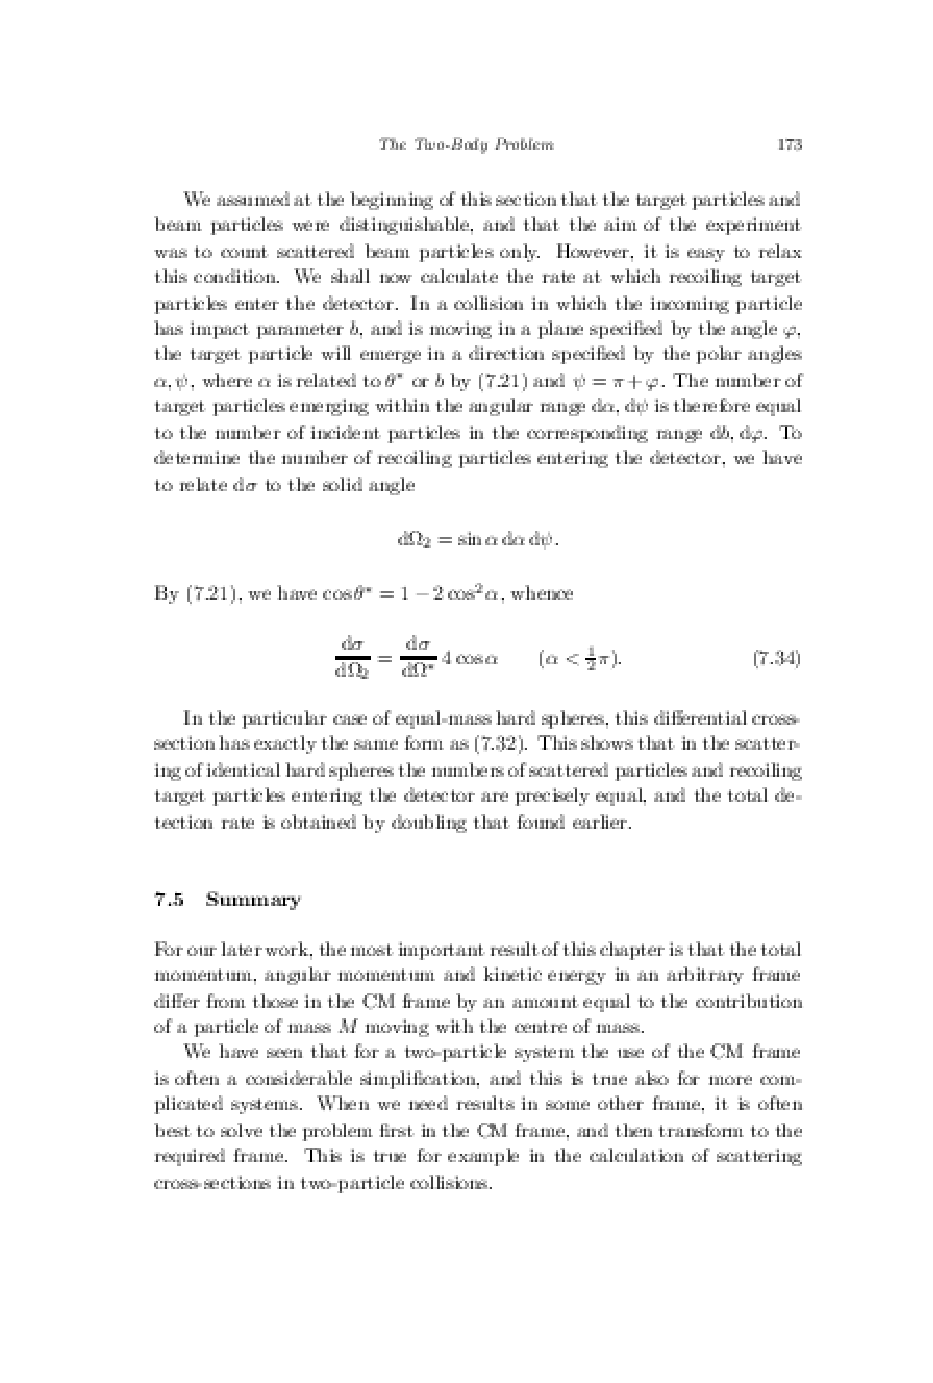
\includegraphics[height=2.51cm]{random-pages/random-pages-from-kibble-pdf-02}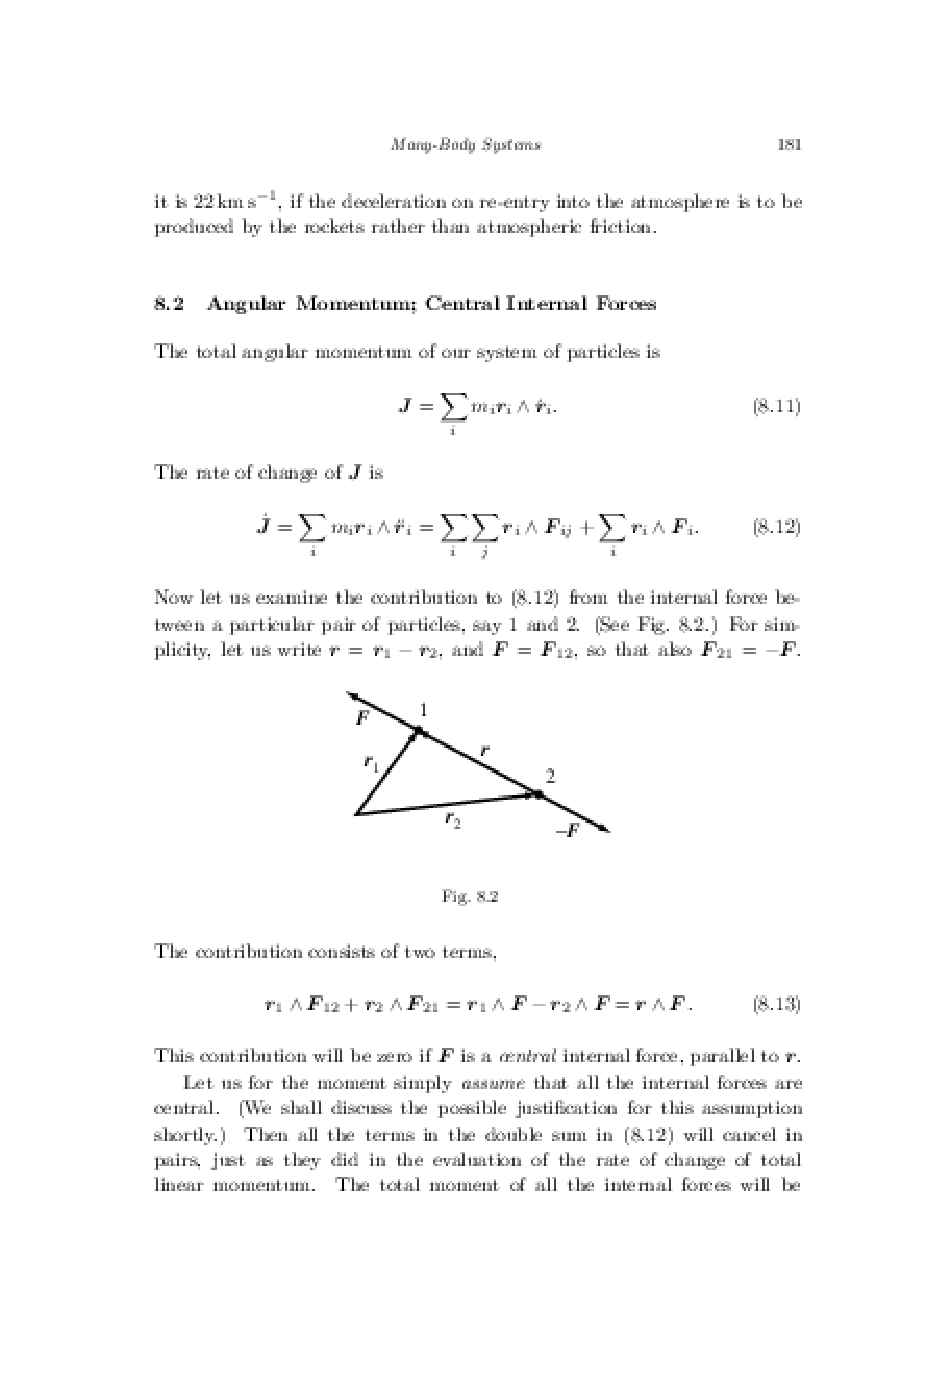
\includegraphics[height=2.51cm]{random-pages/random-pages-from-kibble-pdf-03}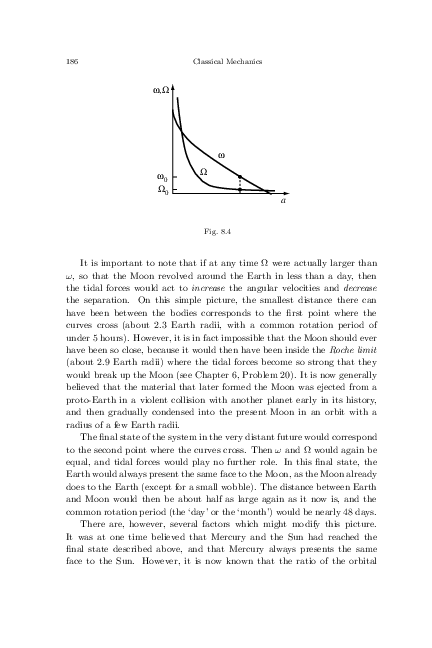
\includegraphics[height=2.51cm]{random-pages/random-pages-from-kibble-pdf-04}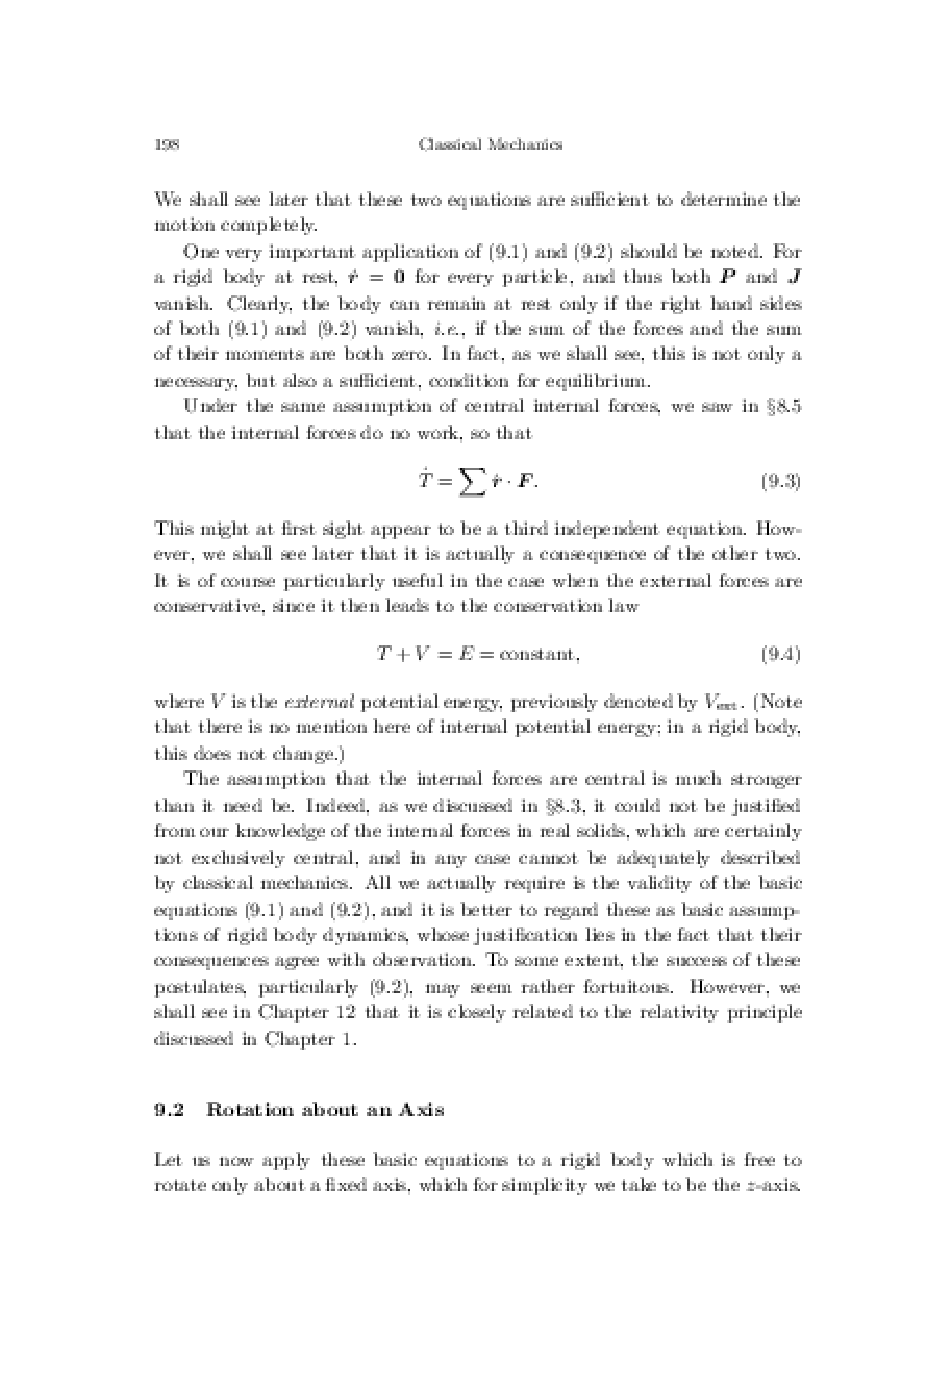
\includegraphics[height=2.51cm]{random-pages/random-pages-from-kibble-pdf-05}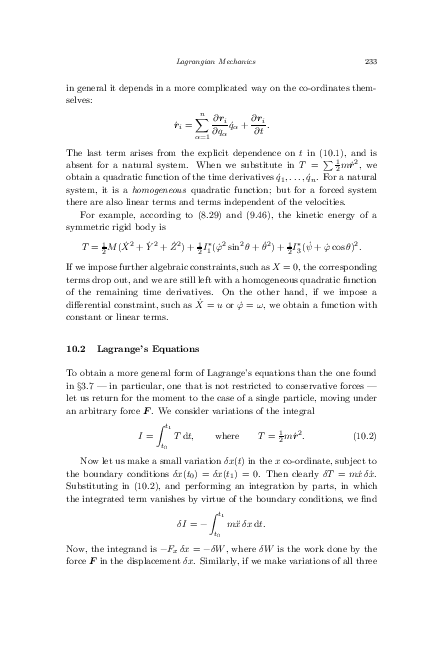
\includegraphics[height=2.51cm]{random-pages/random-pages-from-kibble-pdf-06}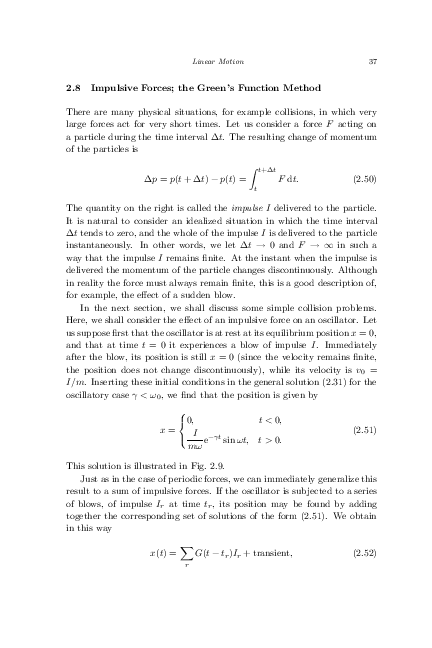
\includegraphics[height=2.51cm]{random-pages/random-pages-from-kibble-pdf-09}
\par\end{centering}
\begin{centering}
\textsf{``}Classical mechanics\textsf{''} by T.~W.~B.~Kibble and F.~H.~Berkshire
(\texttt{\small{}\href{https://archive.org/details/116772449ClassicalMechanics}{https://archive.org/details/116772449ClassicalMechanics}})
\par\end{centering}
\caption{Randomly chosen pages from books on mathematics and physics.\label{fig:Randomly-chosen-pages-2}}
\end{figure}

\begin{figure}
\begin{centering}
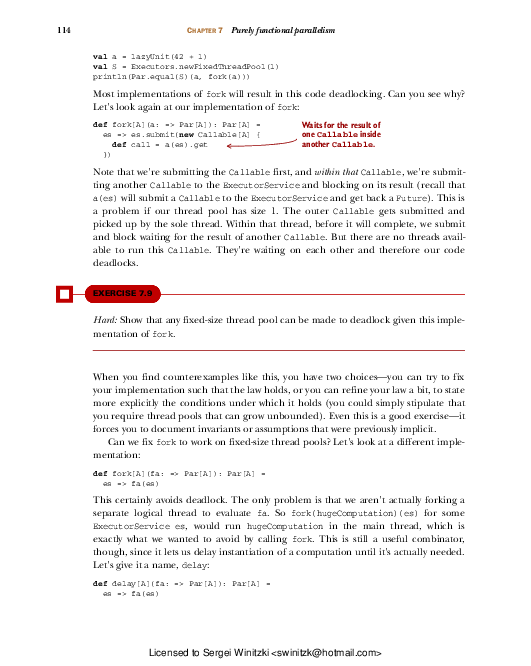
\includegraphics[height=2.51cm]{random-pages/random-pages-from-fpis-pdf-00}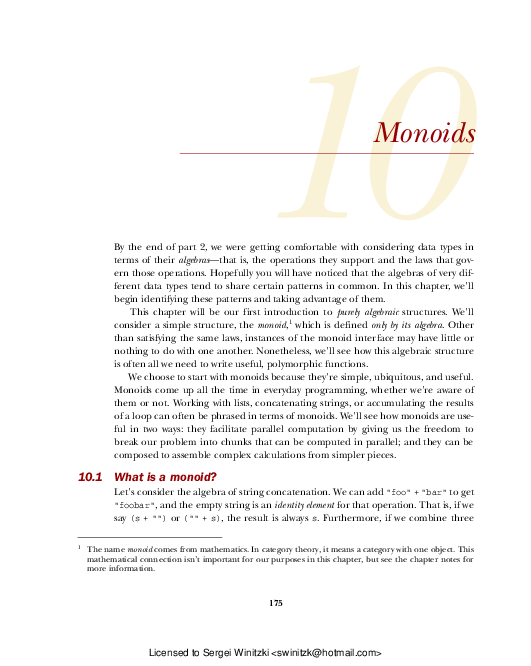
\includegraphics[height=2.51cm]{random-pages/random-pages-from-fpis-pdf-01}\includegraphics[height=2.51cm]{random-pages/random-pages-from-fpis-pdf-02}\includegraphics[height=2.51cm]{random-pages/random-pages-from-fpis-pdf-04}\includegraphics[height=2.51cm]{random-pages/random-pages-from-fpis-pdf-05}\includegraphics[height=2.51cm]{random-pages/random-pages-from-fpis-pdf-06}\includegraphics[height=2.51cm]{random-pages/random-pages-from-fpis-pdf-07}\includegraphics[height=2.51cm]{random-pages/random-pages-from-fpis-pdf-08}
\par\end{centering}
\begin{centering}
\textsf{``}Functional programming in Scala\textsf{''} by P.~Chiusano and R.~Bjarnason
\par\end{centering}
\begin{centering}
\includegraphics[height=2.51cm]{random-pages/random-pages-from-pdbc-pdf-00}\includegraphics[height=2.51cm]{random-pages/random-pages-from-pdbc-pdf-01}\includegraphics[height=2.51cm]{random-pages/random-pages-from-pdbc-pdf-02}\includegraphics[height=2.51cm]{random-pages/random-pages-from-pdbc-pdf-03}\includegraphics[height=2.51cm]{random-pages/random-pages-from-pdbc-pdf-04}\includegraphics[height=2.51cm]{random-pages/random-pages-from-pdbc-pdf-05}\includegraphics[height=2.51cm]{random-pages/random-pages-from-pdbc-pdf-06}\includegraphics[height=2.51cm]{random-pages/random-pages-from-pdbc-pdf-07}
\par\end{centering}
\begin{centering}
\textsf{``}Program design by calculation\textsf{''} by J.~N.~Oliveira
\par\end{centering}
\begin{centering}
\includegraphics[height=2.51cm]{random-pages/random-pages-from-sofp-pdf-00}\includegraphics[height=2.51cm]{random-pages/random-pages-from-sofp-pdf-01}\includegraphics[height=2.51cm]{random-pages/random-pages-from-sofp-pdf-02}\includegraphics[height=2.51cm]{random-pages/random-pages-from-sofp-pdf-05}\includegraphics[height=2.51cm]{random-pages/random-pages-from-sofp-pdf-06}\includegraphics[height=2.51cm]{random-pages/random-pages-from-sofp-pdf-07}\includegraphics[height=2.51cm]{random-pages/random-pages-from-sofp-pdf-08}\includegraphics[height=2.51cm]{random-pages/random-pages-from-sofp-pdf-09}
\par\end{centering}
\begin{centering}
\textsf{''}The science of functional programming\textsf{''} (this book)
\par\end{centering}
\caption{Randomly chosen pages from books on applied functional type theory.\label{fig:Randomly-chosen-pages}}
\end{figure}


\chapter{Essay: Software engineers and software artisans}

Let us look at the differences between the kind of activities we ordinarily
call engineering, as opposed to artisanship or craftsmanship. It will
then become apparent that today\textsf{'}s computer programmers are better
understood as \textsf{``}software artisans\textsf{''} rather than software engineers.

\section{Engineering disciplines }

Consider what kinds of process a mechanical engineer, a chemical engineer,
or an electrical engineer follows in their work, and what kind of
studies they require for proficiency in their work.

A mechanical engineer studies\footnote{\texttt{\href{https://www.colorado.edu/mechanical/undergraduate-students/curriculum}{https://www.colorado.edu/mechanical/undergraduate-students/curriculum}}}
calculus, linear algebra, differential geometry, and several areas
of physics such as theoretical mechanics, thermodynamics, and elasticity
theory, and then uses calculations to guide the design of a bridge,
say. A chemical engineer studies\footnote{\texttt{\href{https://www.colorado.edu/engineering/sample-undergraduate-curriculum-chemical}{https://www.colorado.edu/engineering/sample-undergraduate-curriculum-chemical}}}
chemistry, thermodynamics, calculus, linear algebra, differential
equations, some areas of physics such as thermodynamics and kinetic
theory, and uses calculations to guide the design of a chemical process,
say. An electrical engineer studies\footnote{\texttt{\href{http://archive.is/XYLyE}{http://archive.is/XYLyE}}}
advanced calculus, linear algebra, and several areas of physics such
as electrodynamics and quantum theory, and uses calculations to design
an antenna or a microchip.

The pattern here is that an engineer uses mathematics and natural
sciences in order to design new devices. Mathematical calculations
and scientific reasoning are required \emph{before} drawing a design,
let alone building a real device or machine.

Some of the studies required for engineers include arcane abstract
concepts such as a \textsf{``}rank-4 elasticity tensor\textsf{''}\footnote{\texttt{\href{https://serc.carleton.edu/NAGTWorkshops/mineralogy/mineral_physics/tensors.html}{https://serc.carleton.edu/NAGTWorkshops/mineralogy/mineral\_physics/tensors.html}}}
(used in calculations of elasticity of materials), \textsf{``}Lagrangian with
non-holonomic constraints\textsf{''}\footnote{\texttt{\href{https://arxiv.org/abs/math/0008147}{https://arxiv.org/abs/math/0008147}}}
(used in robotics), the \textsf{``}Gibbs free energy\textsf{''} (for chemical reactor
design\footnote{\texttt{\href{https://www.amazon.com/Introduction-Chemical-Engineering-Kinetics-Reactor/dp/1118368258}{https://www.amazon.com/Introduction-Chemical-Engineering-Kinetics-Reactor/dp/1118368258}}}),
or the \textsf{``}Fourier transform of the delta function\textsf{''}\footnote{\texttt{\href{https://www.youtube.com/watch?v=KAbqISZ6SHQ}{https://www.youtube.com/watch?v=KAbqISZ6SHQ}}}
and the \textsf{``}inverse $Z$-transform\textsf{''}\footnote{\texttt{\href{http://archive.is/SsJqP}{http://archive.is/SsJqP}}}
(for digital signal processing).

To be sure, a significant part of what engineers do is not covered
by any theory: the \emph{know-how}, the informal reasoning, the traditional
knowledge passed on from expert to novice,  \textemdash{} all those
skills that are hard to formalize are important. Nevertheless, engineering
is crucially based on natural science and mathematics for some of
its decision-making about new designs.

\section{Artisanship: Trades and crafts }

Now consider what kinds of things shoemakers, plumbers, or home painters
do, and what they have to learn in order to become proficient in their
profession.

A novice shoemaker, for example, begins by copying some drawings\footnote{\texttt{\href{https://youtu.be/cY5MY0czMAk?t=141}{https://youtu.be/cY5MY0czMAk?t=141}}}
and goes on to cutting leather in a home workshop. Apprenticeships
proceed via learning by doing, with comments and instructions from
an expert. After a few years of study (for example, a painter apprenticeship
in California\footnote{\texttt{\href{http://www.calapprenticeship.org/programs/painter_apprenticeship.php}{http://www.calapprenticeship.org/programs/painter\_apprenticeship.php}}}
can be as short as 2 years), a new artisan is ready to start productive
work. 

All these trades operate entirely from tradition and practical experience.
The trades do not require academic study because there is no formal
theory from which to proceed. Of course, there is \emph{a lot} to
learn in the crafts, and it takes prolonged effort to become a good
artisan in any profession. But there are no rank-4 tensors to calculate,
nor any differential equations to solve; no Fourier transforms applied
to delta functions, and no Lagrangians with non-holonomic constraints.

Artisans do not study science or mathematics because their professions
do not make use of any formal theory for guiding their designs or
processes.

\section{Programmers today are artisans, not engineers }

Programmers are \emph{not engineers} in the sense we normally see
the engineering professions.

\subsection{No requirement of formal study }

According to a recent Stack Overflow survey\footnote{\texttt{\href{https://thenextweb.com/insider/2016/04/23/dont-need-go-college-anymore-programmer/}{https://thenextweb.com/insider/2016/04/23/dont-need-go-college-anymore-programmer/}}},
about 56\% of working programmers do not have a CS degree. The author
of this book is a self-taught programmer who has degrees in physics
but never formally studied computer science or taken any academic
courses in algorithms, data structures, computer networks, compilers,
programming languages, or other computer science topics. 

A large fraction of successful programmers have no college degrees
and perhaps \emph{never} studied formally. They acquired all their
knowledge and skills through self-study and practical work. A prominent
example is Robert C.~Martin\index{Robert C.~Martin}\footnote{\texttt{\href{https://en.wikipedia.org/wiki/Robert_C._Martin}{https://en.wikipedia.org/wiki/Robert\_C.\_Martin}}},
an outspoken guru in the arts of programming. He routinely refers
to programmers as artisans\footnote{\texttt{\href{https://blog.cleancoder.com/uncle-bob/2013/02/01/The-Humble-Craftsman.html}{https://blog.cleancoder.com/uncle-bob/2013/02/01/The-Humble-Craftsman.html}}}
and uses the appropriate imagery: novices and masters, trade and craft,
the honor of the guild, etc. He compares programmers to plumbers,
electricians, lawyers, and surgeons, but never to mathematicians,
physicists, or engineers of any kind. According to one of his blog
posts\footnote{\texttt{\href{https://blog.cleancoder.com/uncle-bob/2013/11/25/Novices-Coda.html}{https://blog.cleancoder.com/uncle-bob/2013/11/25/Novices-Coda.html}}},
he started working at age 17 as a self-taught programmer, and then
went on to more jobs in the software industry; he never mentioned
going to college. It is clear that R.~C.~Martin \emph{is} an expert
craftsman and that he did \emph{not} need academic study to master
his craft.

Here is another opinion\footnote{\texttt{\href{http://archive.is/tAKQ3}{http://archive.is/tAKQ3}}}
(emphasis is theirs):
\begin{quotation}
{\small{}Software Engineering is unique among the STEM careers in
that it absolutely does }\emph{\small{}not}{\small{} require a college
degree to be successful. It most certainly does not require licensing
or certification. }\emph{\small{}It requires experience}{\small{}.}{\small\par}
\end{quotation}
This description fits a career in crafts \textemdash{} but certainly
not a career, say, in electrical engineering.

The high demand for software developers gave rise to \textsf{``}developer
boot camps\textsf{''}\footnote{\texttt{\href{http://archive.is/GkOL9}{http://archive.is/GkOL9}}}
\textemdash{} vocational schools that educate new programmers in a
few months through purely practical training, with no formal theory
or mathematics involved. These vocational schools are successful\footnote{\texttt{\href{http://archive.is/E9FXP}{http://archive.is/E9FXP}}}
in job placement. But it is unimaginable that a $6$-month crash course
or even a $2$-year vocational school could prepare engineers to work
successfully on designing, e.g., analog quantum computers\footnote{\texttt{\href{https://www.dwavesys.com/quantum-computing}{https://www.dwavesys.com/quantum-computing}}}
\emph{without} ever teaching them quantum physics or calculus.

\subsection{No mathematical formalism guides software development}

Most books on software engineering contain no formulas or equations,
no mathematical derivations, and no precise definitions of the various
technical terms they are using (such as \textsf{``}object-oriented\textsf{''} or \textsf{``}module\textsf{'}s
responsibilities\textsf{''}). Some of those books\footnote{E.g., \texttt{\href{https://www.amazon.com/Object-Oriented-Software-Engineering-Unified-Methodology/dp/0073376256}{https://www.amazon.com/Object-Oriented-Software-Engineering-Unified-Methodology/dp/0073376256}}}
also have almost no program code in them; instead they are filled
with words and illustrative diagrams. These books talk about how programmers
should approach their job, how to organize the work flow and the code
architecture, etc., in vague and general terms: \textsf{``}code is about detail\textsf{''},
\textsf{``}you must never abandon the big picture\textsf{''}, \textsf{``}avoid tight coupling
in your modules\textsf{''}, \textsf{``}a class must serve a single responsibility\textsf{''},
and so on. Practitioners such as R.\ C.\ Martin never studied any
formalisms and do not think in terms of formalisms; instead, they
summarize their programming experience in vaguely formulated heuristic
\textquotedblleft principles\textquotedblright .\footnote{\texttt{\href{https://blog.cleancoder.com/uncle-bob/2016/03/19/GivingUpOnTDD.html}{https://blog.cleancoder.com/uncle-bob/2016/03/19/GivingUpOnTDD.html}}}

In contrast, textbooks on mechanical or electrical engineering include
a significant amount of mathematics. The design of a microwave antenna
is guided not by an \textsf{``}open and closed module principle\textsf{''} but by
solving the relevant differential equations\footnote{\texttt{\href{https://youtu.be/8KpfVsJ5Jw4?t=447}{https://youtu.be/8KpfVsJ5Jw4?t=447}}}
of electrodynamics.

Donald Knuth\textsf{'}s classic textbook is called \textsf{``}\emph{The Art of Programming}\textsf{''}.
It is full of tips and tricks about how to program; but it does not
provide any formal theory that could guide programmers in actually
\emph{writing} programs. There is nothing in that book that would
be similar to the way mathematical formalism guides designs in electrical
or mechanical engineering. If Knuth\textsf{'}s books were based on such formalism,
they would have looked quite differently: some theory would be first
explained and then applied to help us write code.

Knuth\textsf{'}s books provide many rigorously derived algorithms. But algorithms
are similar to patented inventions: they can be used immediately without
further study. Understanding an algorithm is not similar to understanding
a mathematical theory. Knowing one algorithm does not make it easier
to develop another algorithm in an unrelated domain. In comparison,
knowing how to solve differential equations will be applicable to
thousands of different areas of science and engineering.

A book exists\footnote{\texttt{\href{https://www.amazon.com/Science-Programming-Monographs-Computer/dp/0387964800}{https://www.amazon.com/Science-Programming-Monographs-Computer/dp/0387964800}}}
with the title \textsf{``}Science of Programming\textsf{''}, but the title is misleading.
The author does not propose a science, similar to physics, at the
foundation of the process of designing programs, similarly to how
calculations in quantum physics predict the properties of a quantum
device. The book claims to give precise methods that guide programmers
in writing code, but the scope of proposed methods is narrow: the
design of simple algorithms for iterative manipulation of data. The
procedure suggested in that book is far from a formal mathematical
\emph{derivation} of programs from specifications. (A book with that
title\footnote{\texttt{\href{https://www.amazon.com/Program-Derivation-Development-Specifications-International/dp/0201416247}{https://www.amazon.com/Program-Derivation-Development-Specifications-International/dp/0201416247}}}
similarly disappoints.) In any case, programmers today are oblivious
to these books and do not use the methods explained there.

Standard computer science courses today do not teach a true \emph{engineering}
approach to software construction. They do teach analysis of programs
using formal mathematical methods; the main such methods are complexity
analysis\footnote{\texttt{\href{https://www.cs.cmu.edu/~adamchik/15-121/lectures/Algorithmic\%20Complexity/complexity.html}{https://www.cs.cmu.edu/$\sim$adamchik/15-121/lectures/Algorithmic\%20Complexity/complexity.html}}}
(the \textsf{``}big-$O$ notation\textsf{''}) and formal verification\footnote{\texttt{\href{https://en.wikipedia.org/wiki/Formal_verification}{https://en.wikipedia.org/wiki/Formal\_verification}}}.
But programs are analyzed or verified only \emph{after} they are somehow
written. Theory does not guide the actual \emph{process} of writing
code, does not suggest good ways of organizing the code (e.g., how
to decompose the code into modules, classes, or functions), does not
tell programmers which data structures and type signatures of functions
will be useful to implement. Programmers make such design decisions
purely on the basis of experience and intuition, trial-and-error,
copy-paste, and guesswork. 

In this context, program analysis and verification is analogous to
writing mathematical equations describing the surface of a shoe made
by a fashion designer. True, the \textsf{``}shoe surface equations\textsf{''} are
mathematically rigorous and can be \textsf{``}analyzed\textsf{''} or \textsf{``}verified\textsf{''};
but the equations are written after the fact and do not guide the
fashion designers in actually making shoes. It is understandable that
fashion designers do not study the mathematical theory of surfaces.

\subsection{Programmers avoid academic terminology }

Programmers jokingly grumble about terms such as \textsf{``}functor\textsf{''}, \textsf{``}monad\textsf{''},
or \textsf{``}lambda-functions\textsf{''}:
\begin{quote}
{\small{}Those fancy words used by functional programmers purists
really annoy me. Monads, functors... Nonsense!!! }\footnote{\texttt{\href{http://archive.is/65K3D}{http://archive.is/65K3D}}}
\end{quote}
Perhaps only a small minority of software developers actually complain
about this; the vast majority seems to remain unaware of \textsf{``}traversable
functors\textsf{''} or \textsf{``}free monads\textsf{''}.

However, chemical engineers accept the need for studying differential
equations and do not mind using the terms \textsf{``}phase diagram\textsf{''} or \textsf{``}Gibbs
free energy\textsf{''}. Electrical engineers do not complain that the word
\textsf{``}Fourier\textsf{''} is difficult to spell, or that \textsf{``}delta-function\textsf{''}
is a weird thing to say. Mechanical engineers take it for granted
that they need to calculate with \textsf{``}tensors\textsf{''} and \textsf{``}Lagrangians\textsf{''}
and \textsf{``}non-holonomic constraints\textsf{''}. The arcane terminology seems
to be the least of their difficulties, as their textbooks are full
of complicated equations and long derivations.

Similarly, software engineers would not complain about the word \textsf{``}functor\textsf{''},
or about having to study the derivation of the algebraic laws for
\textsf{``}monads,\textsf{''} \textemdash{} if they were true engineers. Textbooks
on true software engineering would have been full of equations and
derivations, in order to teach engineers how to perform certain calculations
that are required \emph{before} starting to write code.

\section{Towards true engineering in software}

It is now clear that we do not presently have true software engineering.
The people employed under that job title are actually artisans. They
work using artisanal methods, and their culture and processes are
that of a crafts guild.

True software engineering means having a mathematical theory that
guides the process of writing programs, \textemdash{} not theory that
describes or analyzes programs after they are \emph{somehow} written.

It is true that the numerical methods required for physics or the
matrix calculations required for data science are \textsf{``}mathematical\textsf{''}.
These programming tasks are indeed formulated using mathematical theory.
However, mathematical \emph{subject matter} (aerospace control, physics
or astronomy simulations, or statistics) does not mean that engineering
is used for the process of writing code. Data scientists, aerospace
engineers, and physicists often write programs \textemdash{} but they
almost always work as artisans when implementing their computations
in program code.

We expect that software engineers\textsf{'} textbooks should be full
of equations and derivations. What theory would those equations represent?

This theory is what this book calls \textbf{applied functional type
theory}\index{applied functional type theory} (see Chapter~\ref{chap:Applied-functional-type}).
It is the algebraic foundation of the modern practice of functional
programming, as implemented in languages such as OCaml, Haskell, and
Scala. This theory is a blend of type theory, category theory, and
logical proof theory, adapted for the needs of programmers. It has
been in development since late 1990s and is still being actively worked
on by a community of software practitioners and academic computer
scientists.

To appreciate that functional programming, unlike any other programming
paradigm, has a theory that guides coding, we can look at some recent
software engineering conferences such as \textsf{``}Scala By the Bay\textsf{''}\footnote{\texttt{\href{http://2015.scala.bythebay.io/}{http://2015.scala.bythebay.io/}}}
or BayHac\footnote{\texttt{\href{http://bayhac.org/}{http://bayhac.org/}}},
or at the numerous FP-related online tutorials and blogs. We cannot
fail to notice that speakers devote significant time to a peculiar
kind of applied mathematical reasoning. Rather than focusing on one
or another API or algorithm, as it is often the case with other software
engineering blogs or presentations, an FP speaker describes a \emph{mathematical
structure} \textemdash{} such as the \textsf{``}applicative functor\textsf{''}\footnote{\texttt{\href{http://www.youtube.com/watch?v=bmIxIslimVY}{http://www.youtube.com/watch?v=bmIxIslimVY}}}
or the \textsf{``}free monad\textsf{''}\footnote{\texttt{\href{http://www.youtube.com/watch?v=U0lK0hnbc4U}{http://www.youtube.com/watch?v=U0lK0hnbc4U}}}
\textemdash{} and illustrates its use for practical coding.

These people are not graduate students showing off their theoretical
research; they are practitioners, software engineers who use FP on
their jobs. It is just the nature of FP that certain mathematical
tools \textemdash{} coming from formal logic and category theory \textemdash{}
are now directly applicable to practical programming tasks.

These mathematical tools are not mere tricks for a specific programming
language; they apply equally to all FP languages. Before starting
to write code, the programmer can jot down certain calculations in
a mathematical notation (see Fig.\ \ref{fig:Example-calculation-in-type-theory}).
The results of those calculations will help design the code fragment
the programmer is about to write. This activity is similar to that
of an engineer who performs some mathematical calculations before
embarking on a design project. \begin{wrapfigure}{I}{0.5\textwidth}%
\begin{centering}
{\footnotesize{}\vspace{0.25\baselineskip}
\includegraphics[width=1\linewidth]{ftt-example}\vspace{-0.25\baselineskip}
}{\footnotesize\par}
\par\end{centering}
{\footnotesize{}\caption{A programmer performs a derivation before writing Haskell code.\label{fig:Example-calculation-in-type-theory}}
}{\footnotesize\par}

\vspace{-0.5\baselineskip}
\end{wrapfigure}%
 

A recent example of a development in applied functional type theory
is the \textsf{``}free applicative functor\textsf{''} construction. It was first described
in a 2014 paper\footnote{\texttt{\href{https://arxiv.org/pdf/1403.0749.pdf}{https://arxiv.org/pdf/1403.0749.pdf}}};
a couple of years later, a combined free applicative / free monad
data type was designed and its implementation proposed \footnote{\texttt{\href{https://github.com/typelevel/cats/issues/983}{https://github.com/typelevel/cats/issues/983}}}
as well as in Haskell\footnote{\texttt{\href{https://elvishjerricco.github.io/2016/04/08/applicative-effects-in-free-monads.html}{https://elvishjerricco.github.io/2016/04/08/applicative-effects-in-free-monads.html}}}.
This technique allows programmers to implement declarative side-effect
computations where some parts are sequential but other parts are computed
in parallel, and to achieve the parallelism \emph{automatically} while
maintaining the composability of the resulting programs. The new technique
has distinct advantages over using monad transformers, which was a
previously used method of composing declarative side-effects. The
combined \textsf{``}free applicative / free monad\textsf{''} was designed and implemented
by true software engineers. They first derived the type constructor
that has the necessary algebraic properties. Guided by the resulting
type formula, they wrote the code that was guaranteed to work.

Another example of applied functional type theory is the  \textsf{``}\index{tagless final}tagless
final\textsf{''} encoding of effects, first described\footnote{\texttt{\href{http://okmij.org/ftp/tagless-final/index.html}{http://okmij.org/ftp/tagless-final/index.html}}}
in 2009. That technique (called \textsf{``}Church-encoded free monad\index{free monad}\textsf{''}
in the present book) has several advantages over the ordinary free
monad and can improve upon it in a number of cases \textemdash{} just
as the free monad itself was designed to cure certain problems with
monad transformers\footnote{\texttt{\href{http://blog.ezyang.com/2013/09/if-youre-using-lift-youre-doing-it-wrong-probably/}{http://blog.ezyang.com/2013/09/if-youre-using-lift-youre-doing-it-wrong-probably/}}}.
The new encoding is not tied to a specific programming language. Rather,
it is a language-agnostic construction that was originally described
in OCaml and later used in Haskell and Scala, but can be made to work
even in Java\footnote{\texttt{\href{http://archive.is/rLAh9}{http://archive.is/rLAh9}}},
which is not an FP language.

This example shows that we may need several more years of work before
the practical aspects of using applied functional type theory are
sufficiently well understood by the FP community. The theory is in
active development, and its design patterns \textemdash{} as well
as the exact scope of the requisite theoretical material \textemdash{}
are still being figured out. If the 40-year gap hypothesis\footnote{\texttt{\href{http://archive.is/rJc4A}{http://archive.is/rJc4A}}}
holds, we should expect applied functional type theory (perhaps under
a different name) to become mainstream by 2030. This book is a step
towards a clear designation of the scope of that theory.

\section{Does software need engineers, or are artisans good enough? }

The demand for programmers is growing. \textsf{``}Software developer\textsf{''} was
\#1 best job\footnote{\texttt{\href{http://archive.is/cGJ2T}{http://archive.is/cGJ2T}}}
in the US in 2018. But is there a demand for engineers or just for
artisans?

We do not seem to be able to train enough software artisans.\footnote{\texttt{\href{http://archive.is/137b8}{http://archive.is/137b8}}}
So, it is probably impossible to train as many software engineers
in the true sense of the word. Modern computer science courses do
not actually train engineers in that sense; at best, they train academic
researchers who write code as software artisans. Recalling the situation
in construction business, with a few architects and hundreds of construction
workers, we might also conclude that, perhaps, only a few software
engineers are required per hundred software artisans.

What is the price of \emph{not} having engineers, of replacing them
with artisans?

Software practitioners have long bemoaned the mysterious difficulty
of software development. Code \textsf{``}rots with time\textsf{''}, its complexity
grows \textsf{``}out of control\textsf{''}, and operating systems have been notorious
for ever-appearing security flaws\footnote{\texttt{\href{http://archive.fo/HtQzw}{http://archive.fo/HtQzw}}}
despite many thousands of programmers and testers employed. Clearly,
we overestimated the capacity of the human brain for artisanal programming.

It is precisely in designing large and robust software systems that
we would benefit from true engineering. Artisans has been building
bridges and using chemical reactions by trial and error and via tradition,
long before mechanical or chemical engineering disciplines were developed
and founded upon rigorous theory. But once the theory became available,
engineers were able to design unimaginably more powerful and complicated
structures, devices, and processes. It is clear that trial, error,
and adherence to tradition is inadequate for some of the software
development tasks in front of us. 

To build large and reliable software, such as new mobile or embedded
operating systems or distributed peer-to-peer trust architectures,
we will most likely need the qualitative increase in productivity
and reliability that can only come from replacing artisanal programming
by a true engineering discipline. Applied functional type theory and
functional programming are steps in that direction.

\chapter{Essay: Towards functional data engineering with Scala}

Data engineering is among the most in-demand\footnote{\texttt{\href{http://archive.is/mK59h}{http://archive.is/mK59h}}}
novel occupations in the IT world today. Data engineers create software
pipelines that process large volumes of data efficiently. Why did
the Scala programming language emerge as a premier tool\footnote{\texttt{\href{https://www.slideshare.net/noootsab/scala-the-unpredicted-lingua-franca-for-data-science}{https://www.slideshare.net/noootsab/scala-the-unpredicted-lingua-franca-for-data-science}}}
for crafting the foundational data engineering technologies such as
Spark or Akka? Why is Scala in high demand\footnote{\texttt{\href{https://techcrunch.com/2016/06/14/scala-is-the-new-golden-child/}{https://techcrunch.com/2016/06/14/scala-is-the-new-golden-child/}}}
within the world of big data?

There are reasons to believe that the choice of Scala was not accidental.

\section{Data is math}

Humanity has been working with data at least since Babylonian tax
tables\footnote{\texttt{\href{https://www.nytimes.com/2017/08/29/science/trigonometry-babylonian-tablet.html}{https://www.nytimes.com/2017/08/29/science/trigonometry-babylonian-tablet.html}}}
and the ancient Chinese number books\footnote{\texttt{\href{http://quatr.us/china/science/chinamath.htm}{http://quatr.us/china/science/chinamath.htm}}}.
Mathematics summarizes several millennia\textsf{'}s worth of data processing
experience in a few fundamental tenets:

\begin{wrapfigure}{I}{0.34\columnwidth}%
\begin{centering}
\vspace{-0.65\baselineskip}
\includegraphics[width=0.96\linewidth]{type-error}\vspace{-0.5\baselineskip}
\par\end{centering}
\caption{Mixing incompatible data types produces nonsensical results.\label{fig:A-nonsensical-calculation}}

\vspace{-3.5\baselineskip}
\end{wrapfigure}%

\begin{itemize}
\item Data is \emph{immutable}, because facts are immutable. 
\item Each \emph{type} of values (population count, land area, distances,
prices, times, etc.) needs to be handled separately; it is meaningless
to add a distance to a population count.
\item Data processing should be performed according to \emph{mathematical
formulas}. 
\end{itemize}
Violating these tenets produces nonsense (see Fig.\ \ref{fig:A-nonsensical-calculation}
for a real-life illustration).

The power of the principles of mathematics extends over all epochs
and all cultures; math is the same in San Francisco, in Rio de Janeiro,
in Kuala-Lumpur, and in Pyongyang (Fig.\ \ref{fig:The-Pyongyang-method-of-error-free-programming}).

\section{Functional programming is math}

The functional programming paradigm is based on mathematical principles:
values are immutable, data processing is coded through formula-like
expressions, and each type of data is required to match correctly
during the computations. The type-checking process automatically prevents
programmers from making many kinds of coding errors. In addition,
programming languages such as Scala and Haskell have a set of features
adapted to building powerful abstractions and domain-specific languages.
This power of abstraction is not accidental. Since mathematics is
the ultimate art of building abstractions, math-based functional programming
languages capitalize on the advantage of millennia of mathematical
experience.

A prominent example of how mathematics informs the design of programming
languages is the connection between constructive logic\footnote{\texttt{\href{https://en.wikipedia.org/wiki/Intuitionistic_logic}{https://en.wikipedia.org/wiki/Intuitionistic\_logic}}}
and the programming language\textsf{'}s type system, called the Curry-Howard
(CH) correspondence\footnote{\texttt{\href{https://en.wikipedia.org/wiki/Curry\%E2\%80\%93Howard_correspondence}{https://en.wikipedia.org/wiki/Curry\%E2\%80\%93Howard\_correspondence}}}.
The main idea of the CH correspondence\index{Curry-Howard correspondence}
is to think of programs as mathematical formulas that compute a value
of a certain type $A$. The CH correspondence is between programs
and logical propositions: To any program that computes a value of
type $A$, there corresponds a proposition stating that \textsf{``}a value
of type $A$ can be computed\textsf{''}.

This may sound rather theoretical so far. To see the real value of
the CH correspondence, recall that formal logic has operations \textsf{``}\textbf{\emph{and}}\textsf{''},
\textsf{``}\textbf{\emph{or}}\textsf{''}, and \textsf{``}\textbf{\emph{implies}}\textsf{''}. For any
two propositions $A$, $B$, we can construct the propositions \textsf{``}$A$
\textbf{\emph{and}} $B$\textsf{''}, \textsf{``}$A$ \textbf{\emph{or}} $B$\textsf{''}, \textsf{``}$A$
\textbf{\emph{implies}} $B$\textsf{''}. These three logical operations are
foundational; without one of them, the logic is \emph{incomplete}
(you cannot derive some theorems).

A programming language \textbf{obeys the CH correspondence}\index{Curry-Howard correspondence}
with the logic if for any types $A$, $B$, the language also contains
composite types corresponding to the logical formulas \textsf{``}$A$ \textbf{\emph{or}}
$B$\textsf{''}, \textsf{``}$A$ \textbf{\emph{and}} $B$\textsf{''}, \textsf{``}$A$ \textbf{\emph{implies}}
$B$\textsf{''}. In Scala, these composite types are \texttt{Either{[}A,B{]}},
the tuple \texttt{(A,B)}, and the function type, \texttt{A$\rightarrow$B}.
All modern functional languages such as OCaml, Haskell, Scala, F\#,
Swift, Elm, and PureScript support these three type constructions
and thus are faithful to the CH correspondence. Having a \emph{complete}
logic in a language\textsf{'}s type system enables declarative domain-driven
code design\footnote{\texttt{\href{https://fsharpforfunandprofit.com/ddd/}{https://fsharpforfunandprofit.com/ddd/}}}.

\begin{wrapfigure}{I}{0.5\columnwidth}%
\begin{centering}
\vspace{-0.5\baselineskip}
\includegraphics[width=1\linewidth]{no-bugs}\vspace{-0.5\baselineskip}
\par\end{centering}
\caption{The Pyongyang method of error-free software engineering.\label{fig:The-Pyongyang-method-of-error-free-programming}}
\vspace{-3\baselineskip}
\end{wrapfigure}%

It is interesting to note that most older programming languages (C/C++,
Java, JavaScript, Python) do not support some of these composite types.
In other words, these programming languages have type systems based
on an incomplete logic. As a result, users of these languages have
to implement burdensome workarounds that make for error-prone code.
Failure to follow mathematical principles has real costs (Figure~\ref{fig:The-Pyongyang-method-of-error-free-programming}).

\section{The power of abstraction}

Early adopters of Scala, such as Netflix, LinkedIn, and Twitter, were
implementing what is now called \textsf{``}big data engineering\textsf{''}. The required
software needs to be highly concurrent, distributed, and resilient
to failure. Those software companies used Scala as their main implementation
language and reaped the benefits of functional programming.

What makes Scala suitable for big data tasks? The only reliable way
of managing massively concurrent code is to use sufficiently high-level
abstractions that make application code declarative. The two most
important such abstractions are the \textsf{``}resilient distributed dataset\textsf{''}
(RDD) of Apache Spark and the \textsf{``}reactive stream\textsf{''} used in systems
such as Kafka, Akka Streams, and Apache Flink. While these abstractions
are certainly implementable in Java or Python, a fully declarative
and type-safe usage is possible only in a programming language with
a sophisticated type system. Among the currently available mature
functional languages, only Scala and Haskell are technically adequate
for that task, due to their support for typeclasses and higher-order
types. The early adopters of Scala were able to benefit from the powerful
abstractions Scala supports. In this way, Scala enabled those businesses
to engineer and to scale up their massively concurrent computations.

It remains to see why Scala and not, say, Haskell became the \emph{lingua
franca} of big data.

\section{Scala is Java on math }

The recently invented general-purpose functional programming languages
can be grouped into \textsf{``}industrial\textsf{''} (F\#, Scala, Swift) and \textsf{``}academic\textsf{''}
(OCaml, Haskell).

The \textsf{``}academic\textsf{''} languages are clean-room implementations of well-researched
mathematical principles of programming language design (the CH correspondence
being one such principle). These languages are unencumbered by requirements
of compatibility with any existing platform or libraries. Because
of this, the \textsf{``}academic\textsf{''} languages are perfect playgrounds for
taking various mathematical ideas to their logical conclusion. At
the same time, software practitioners struggle to adopt these languages
due to a steep learning curve, a lack of enterprise-grade libraries
and tool support, and immature package management.

The languages from the \textsf{``}industrial\textsf{''} group are based on existing
and mature software ecosystems: F\# on .NET, Scala on JVM, and Swift
on the MacOS/iOS platform. One of the important design requirements
for these languages is 100\% binary compatibility with their \textsf{``}parent\textsf{''}
platforms and languages (F\# with C\#, Scala with Java, and Swift
with Objective-C). Because of this, developers can immediately take
advantage of the existing tooling, package management, and industry-strength
libraries, while slowly ramping up the idiomatic usage of new language
features. However, the same compatibility requirements dictated certain
limitations in the languages, making their design less than fully
satisfactory from the functional programming viewpoint.

It is now easy to see why the adoption rate of the \textsf{``}industrial\textsf{''}
group of languages is much higher\footnote{\texttt{\href{https://www.tiobe.com/tiobe-index/}{https://www.tiobe.com/tiobe-index/}},
archived in 2019 at \texttt{\href{http://archive.is/RsNH8}{http://archive.is/RsNH8}}} than that of the \textsf{``}academic\textsf{''} languages. The transition to the
functional paradigm is also smoother for software developers because
F\#, Scala, and Swift seamlessly support the familiar object-oriented
programming paradigm. At the same time, these new languages still
have logically complete type systems, which gives developers an important
benefit of type-safe domain modeling.

Nevertheless, the type systems of these languages are not equally
powerful. For instance, F\# and Swift are similar to OCaml in many
ways but omit OCaml\textsf{'}s parameterized modules and some other features.
Of all mentioned languages, only Scala and Haskell directly support
typeclasses and higher-order types, which are helpful for expressing
abstractions such as automatically parallelized data sets or asynchronous
data streams.

To see the impact of these advanced features, consider LINQ, a domain-specific
language for database queries on .NET, implemented in C\# and F\#
through a special built-in syntax supported by Microsoft\textsf{'}s compilers.
Analogous functionality is provided in Scala as a \emph{library},
without need to modify the Scala compiler, by several open-source
projects such as Slick, Squeryl, or Quill. Similar libraries exist
for Haskell \textemdash{} but not in languages with less powerful
type systems.

\section{Summary}

The decisive advantages of Scala over other contenders (such as OCaml,
Haskell, F\#, or Swift) are:
\begin{enumerate}
\item Functional collections in the standard library.
\item A sophisticated type system with support for typeclasses and higher-order
types.
\item Seamless compatibility with a mature software ecosystem (JVM).
\end{enumerate}
Based on this assessment, we may be confident in Scala\textsf{'}s great future
as a main implementation language for big data engineering. 
